\chapter{螺管实例,HTS磁体和结论}
\section{引言}
本章包括三个部分。第一部分给出多个螺管磁体实例,各范例均有问题与解答(Q/A)。
第二部分讨论HTS磁体应用及其前景。
最后有一个简明的结论性评论。

这里描述和研究的四个螺管磁体实例的选取,不是因为他们特别重要或唯一---
没有哪个磁体系统是唯一的,不过对某些人而言,每一个磁体都是唯一的。
选取这几个例子,主要还是因为作者对这些磁体的熟悉。
在描述部分之后的Q/A部分,前面七章涉及的设计和运行的若干要点,再次提出。

这里,我们再次强调一下第一章中已经阐述过的我们的基本哲学:
任何问题,需要数值解的,首先应该使用经得起数值解检验的简化模型得到近似估计。
近似估计快速告诉磁体设计者磁体是否在正确的轨道上。
对于任何简单或复杂的磁体,该工作都很重要。
``创新"磁体的想法通常始于个人。
 为了评估这个想法是否切合实际并且值得与同事进一步深入研究甚至组建设计团队,
 发起人必须首先计算设计和运行关键参数的大概值(第2-8章所述),从简单参数如总安匝数、整体运行电流密度、磁体尺寸和重量、导体总长度,到更复杂的如稳定性和保护、力和低温要求。
 这里的关键词是近似:在磁体项目的后期阶段,设计团队的专家将使用复杂的程序来计算准确的参数值。
 将确切的值留给专家,但要准备好确认他们确实属于独立计算的近似数字范围。
 作者希望在研究了第2-8章后,读者---电磁场、应力、低温、甚至材料领域的专家---
 将能够处理下面提出的四个磁体示例中包含的大多数问题。


\section{螺管磁体实例}
实例中描述和研究的四个螺管磁体是:
1)  由一个大型超导磁体和一个电阻性内插磁体组成的混合磁体;
2) 钢板上的磁体;
3) 一个由螺管磁体产生的磁场悬浮起来的HTS板(盘片);
4) 层叠HTS环片组成的``螺管"磁体,HTS环片由块材或涂层导体板制成。 


\subsection{例A:串联混合磁体}
NHMFL建造的中心轴向场35-40 T(取决于室温孔大小,32-50 mm)的高场磁体,由
一个超导磁体和一个5线圈高均匀电阻性(水冷)内插磁体组成。
因为超导磁体和5线圈电阻性内插磁体电气上串联且由同一个DC电源供电,
磁体被称为``串联混合磁体"(series-connected-hybrid, SCH)。
SCH产生的中心场大于NHMFL所有的电阻性磁体的磁场(35 T)或全超导磁体的磁场(21 T)。
图9.1给出了SCH磁体的剖面示意图---
参数值与SCH磁体的最终采纳值略有不同。

SCH还包括一个薄($\alpha\simeq 1$)的超导屏蔽线圈,绕组半径约1 m,图中未画出。
屏蔽线圈的反极性的,用以减小SCH磁体的边缘场。
在Q/A部分,我们将计算超导屏蔽线圈要求的安匝数近似值。
同时,我们还将设计可作为技术备选的钢圆柱壳屏蔽系统。
\begin{figure}[htbp]
	\centering
	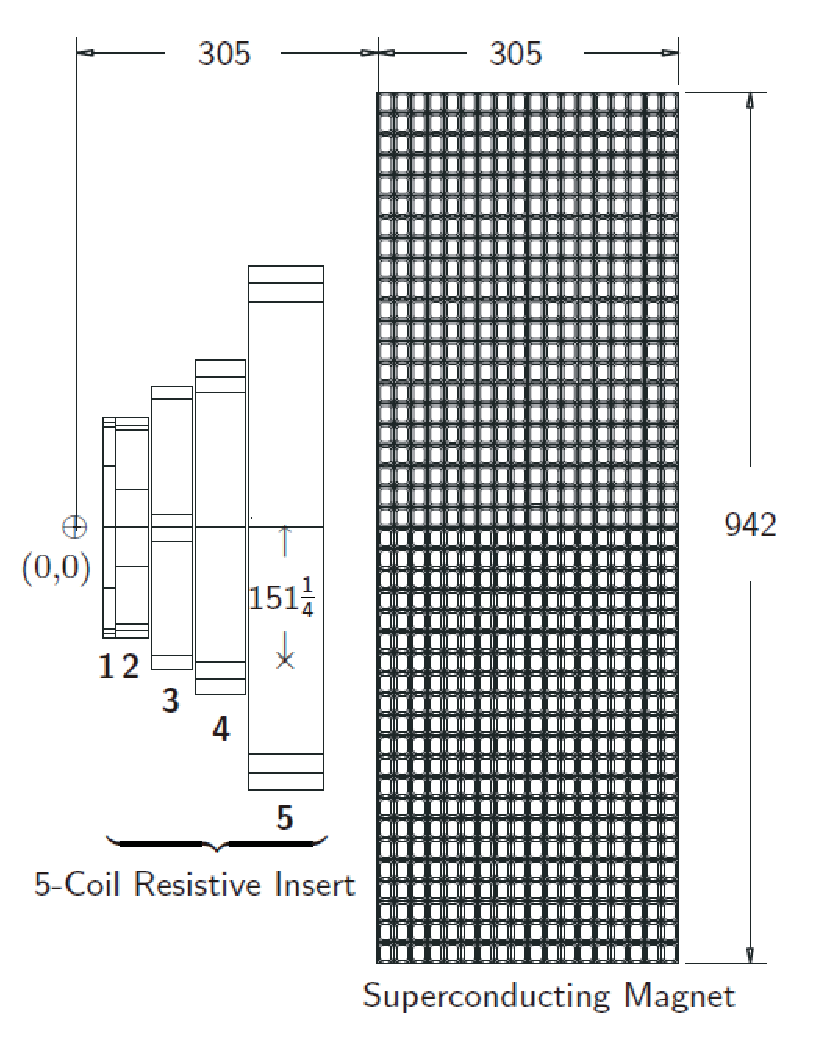
\includegraphics[scale=0.7]{chpt9/figs/fig9.1.eps}
	\caption{NHMFL的SCH磁体的一半结构的剖视图---
		半径约1 m的超导屏蔽线圈未画出。绕组的尺度为近似值,以mm为单位;
	线圈5的$\times$号表示它在故障模式后的磁场中心---将在Q/A部分讨论。}
\end{figure}

\begin{figure}[htbp]
	\centering
	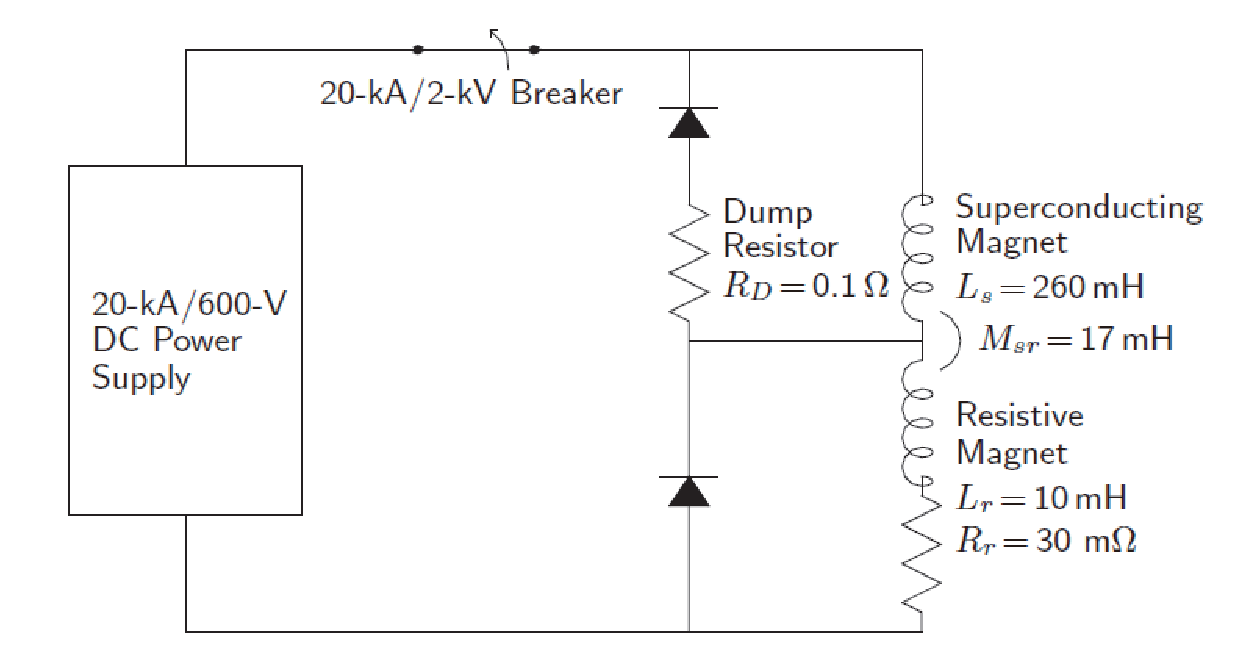
\includegraphics[scale=0.6]{chpt9/figs/fig9.2.eps}
	\caption{SCH磁体的等效电路图。[NHMFL授权使用,2005]}
\end{figure}

图9.2给出了SCH的等效电路图。其中,超导磁体(自感$L_s$=260 mH)与电阻性磁体(自感$L_r$=10 mH,电阻$R_r$=30 m$\Omega$)串联。
磁体由一个20 kA/600 V电源供电。
保护方面,超导磁体用$R_D$=0.1 $\Omega$泄放电阻和二极管串联组作为旁路;
电阻性磁体使用二极管旁路。
(假设两个二极管都是理想的,即正向电阻为零,反向电阻无穷大。)
如图9.2所示,两个磁体间互感$M_{sr}$为17 mH。
在任一磁体异常时,打开20 kA/2 kV断路器。

表9.1列出了超导磁体和该磁体最内层使用的CIC导体的关键参数值。
其中的$A_{sc},A_{\bar{m}},A_{m},A_{cl}$分别是$\mathrm{Nb_3 Sn}$ CIC导体的截面、非基底金属截面、基底金属(铜)截面、4.5 K超临界氦截面。

\begin{table}[htbp]\small
\centering
\caption{超导磁体和CIC导体的参数}  %表9.1 
\begin{tabular}{|c|c|}
\hline
\multicolumn{1}{|l|}{参数} & 数值 \\ \hline
\multirow{7}{*}{\begin{tabular}[c]{@{}c@{}}超导磁体\\ 绕组内径i.d.($2a_1$) $\left[\mathrm{mm}\right]$ \\ 绕组外径o.d.($2a_2$) $\left[\mathrm{mm}\right]$\\ 绕组高度($2b$) $\left[\mathrm{mm}\right]$\\ 匝数/层\\ 层数\\ 总匝数(N)\end{tabular}} & \\ \cline{2-2} 
& 610.0 \\ \cline{2-2} 
& 1220.2 \\ \cline{2-2} 
& 942.0 \\ \cline{2-2} 
& 42 \\ \cline{2-2} 
& 18 \\ \cline{2-2} 
& 756 \\ \hline
\multirow{4}{*}{\begin{tabular}[c]{@{}c@{}}CIC导体@最内层\\ $A_{sc}+A_{\bar{m}}$ $\left[\mathrm{mm^2}\right]$\\ $A_m$ $\left[\mathrm{mm^2}\right]$\\ $A_{cl}$ $\left[\mathrm{mm^2}\right]$ \end{tabular}} & \\ \cline{2-2} 
& 40.2 \\ \cline{2-2} 
& 57.4 \\ \cline{2-2} 
& 76.0 \\ \hline
\end{tabular}
\end{table}


\subsubsection{Q/A A:SCH超导磁体}
\textbf{a) 总体电流密度}\qquad 超导磁体在其运行电流$I_{op}$=20 kA时的总体临界电流密度$\lambda J_{op}$是多少?

\textbf{解:}应用方程3.108a,代入$N$=756和$I=I_{op}$=20 kA,我们得到:
\begin{align*}% page548 第1个
\lambda J_{op}&=\frac{NI}{2b(a_2-a_1)}\\ \tag{3.108a}
&=\frac{756(20\times10^3\ \mathrm{A})}{(942.0\ \mathrm{mm})(610.1\ \mathrm{mm}-305.0\ \mathrm{mm})}=52.6\ \mathrm{A/mm^2}
\end{align*}

\textbf{b) 中心场}\qquad 超导磁体在$I_{op}$=20 kA时,在中心位置产生的磁场(磁感应强度)$B_z(0,0)$是多少?

\textbf{解:}类似的,由表9.1,我们有$\alpha=$1220.2/610.0=2.00;$\beta$=942.0/610.0=1.544。
使用方程3.110,有:
\begin{align*}% page548 第3个
B_{z}(0,0)=\frac{\mu_oNI}{2a_1(\alpha-1)}\ln(\frac{\alpha+\sqrt{\alpha^2+\beta^2}}{1+\sqrt{1+\beta^2}}) \tag{3.110}
\end{align*}

于是,
\begin{align*}% page548 第4个
B_z(0,0)&=\frac{(4\pi\times10^{-7}\ \mathrm{H/m})(756)(20\times10^3\ \mathrm{A})}{(0.610\ \mathrm{m})(2.00-1)}\ln(\frac{2.00+\sqrt{(2.00)^2+(1.544)^2}}{1+\sqrt{1+(1.544)^2}})\\
&=14.52\ \mathrm{T}
\end{align*}

\textbf{c) 中平面径向场}\qquad 超导磁体在中平面($z=0$)的$R=a_2$处产生的磁场的径向分量$B_r(z=0,r=2a_2)$是多少?

\textbf{解:}理想螺管磁体或嵌套线圈磁体产生的磁场的径向分量关于中平面对称,所以总是零:$B_r(0,a_2)=0$

\textbf{d) 电感}\qquad 使用方程3.81和3.14计算磁体自感$L_s$的近似值。如前所述,准确值是260 mH。

\textbf{解:}使用方程3.81和3.14,$\mathcal{L}(\alpha=2.00,\beta=1.544)\simeq 1.2$,我们有:
\begin{align*}% page548 第5个
L&=\mu_oa_1N^2\ \mathcal{L}(\alpha,\beta) \\\tag{3.81}
L_s&=(4\pi\times10^{-7}\ \mathrm{H/m})(0.305\ \mathrm{m})(756)^2(1.2)=263\ \mathrm{mH}
\end{align*}

\textbf{e) 储存的磁能}\qquad 超导磁体在运行电流$I_{op}$=20 kA时储存的总磁能$E_{ms}$是多少?

\textbf{解:}此处我们必须考虑互感的影响。所以:
\begin{align*}% page548 第7个
E_{ms}=&\frac{1}{2}(L_s+M_{sr})I_{op}^2\\
=&\frac{1}{2}(260\ \mathrm{mH}+17\ \mathrm{mH})(20\ \mathrm{kA})^2=55.4\ \mathrm{MJ}
\end{align*}

\textbf{f) 二极管}\qquad 解释与电阻$R_D$串联的二极管的两个功能。

\textbf{解:}反向串联的二极管有两个作用:1) 当磁体励磁时,防止电流通过$R_D$,即令100\%的电源电流都进入磁体;
2) 当开关打开时,允许电流通过$R_D$放电。

\textbf{g) 充电电压}\qquad 恒充电速率400 A/s,$dI_s/dt=dI_r/dt=dI_S/dt$=400 A/s,其中,$I_s$是通过超导
磁体的电流,$I_r$是通过电阻性磁体的电流,$I_S$是电源电流。那么,$I_s=I_r=I_S$=10 kA时,要求的电源电压$V_S$是多少?

\textbf{解:}电源电压为:
\begin{align*}% page549 第1个
V_S&=L_s\frac{dI_s}{dt}+M_{sr}\frac{dI_r}{dt}+M_{sr}\frac{dI_s}{dt}+L_r\frac{dI_r}{dt}+R_rL_r\\
&=(L_s+2M_{sr}+L_r)\frac{dI_s}{dt}+R_rI_S \tag{g.1}
\end{align*}

代入合适的值,有:
\begin{align*}% page549 第3个
V_S=(260\ \mathrm{mH}+2\times17\ \mathrm{mH}+10\ \mathrm{mH})(400\ \mathrm{A/s})+(30\ \mathrm{m\Omega})(10\ \mathrm{kA})=421.6\ \mathrm{kA}
\end{align*}

\textbf{h) 功率}\qquad 当充电速率为$dI_S/dt$=400 A/s,$I_S$=10 kA时,电源供给磁体(含超导和电阻部分)的总的瞬时功率$P_S$为多少?

\textbf{解:}如\textbf{g)},我们有:
\begin{align*}% page549 第4个
V_S&=(L_s+2M_{sr}+L_r)\frac{dI_S}{dt}+R_rI_S\\ \tag{g.1}
&=421.6\ \mathrm{V}
\end{align*}

$P_S=V_S I_S$;于是,$P_S$=4.216 MW。
我们注意到,在4.216 MW中,有1.216 MW[=4.216 MW-(30 m$\Omega$)$\times(10\ \mathrm{kA})^2$]
是无功功率,即存储于两个磁体中的磁能。
随着电源的电流减为零,磁能会``返回"到电源中。

\textbf{i) 600 V电源电压}\qquad 证明在这个电流增长率(400 A/s)下,电源
最大电压600 V在$I_S\simeq$16 kA时达到。

\textbf{解:}要求的总感性电压$V_{ind}$为:
\begin{align*}% page550 第1个
V_{ind}=(L_s+2M_{sr}+L_r)\frac{dI_S}{dt}
\end{align*}
其中,在$dI_S/dt$=400 A/s时,上式成为:
\begin{align*}% page550 第2个
V_{ind}=(260\ \mathrm{mH}+2\times17\ \mathrm{mH}+10\ \mathrm{mH})(400\ \mathrm{A/s})=121.6\ \mathrm{V}
\end{align*}

同时我们还有:$V_S=V_{ind}+R_rI_r$。代入相应的值,有:$I_r$=15946.7 A;$I_S\simeq$16 kA。

\textbf{j) 16 kA$\rightarrow$20 kA充电时间}\qquad 证明在电流超过16 kA($I_{16}$)之后,
如果电源电压维持600 V,电流将在约1分钟内达到运行电流20 kA($I_{20}$)的$\sim$10 A偏差限内。

\textbf{解:}当电流达到16 kA时,电源的电压不能维持充电速率400 A/s。
在$I_s(t)\ge I_{16}$=16 kA时,$I_s(t)=I_{20}+(I_{20}-I_{16}[1-e^(-t/\tau)])$。
其中,$I_{20}$=20 kA,$\tau$是有效电路时间常数,约为10 s,由总有效电感304 mH(=260 mH+(2$\times$17 mH)+10 mH)
除以30 m$\Omega$得到。
在6个时间常数,也即1分钟内,总电流将达到20 kA的10 A($\simeq 4000 e^{-6}$)偏差限内。

\textbf{k) CIC---氦流量}\qquad CIC导体的氦流截面积为$A_{cl}=76.0\ \mathrm{ mm^2}$(表9.1)。
通道中流过3.5 atm和4.5 K的超临界氦,流量为$\.{m}_{he}$=5 g/s。
证明,流动是湍流,雷诺数Re$\simeq 10^5$。
使用下面的参数:氦密度$\rho_{he}=0.132\ \mathrm{g/cm^3}$;
氦黏度$\nu_{he}=35.9\times 10^{-6}\ \mathrm{g/cm\cdot s}$;
水力直径$D_{he}=$1 cm。

\textbf{解:} 流体速度$\v_{he}$由$\.{m}_{he}=\varrho_{he}A_{cl}v_{he}$给出。于是:
\begin{align*}% page550 第4个
v_{he}&=\frac{\.{m}_{he}}{\varrho_{he}A_{cd}}\\
&=\frac{(5\ \mathrm{g/s})}{(0.132\ \mathrm{g/cm^3})(0.760\ \mathrm{cm^2})}\simeq50\ \mathrm{cm/s}
\end{align*}

雷诺数Re为:
\begin{align*}% page550 第6个
R_e&=\frac{\varrho_{he}v_{he}D_{he}}{\nu_{he}}\\
&\simeq\frac{(0.132\ \mathrm{g/cm^3})(50\ \mathrm{cm/s})(1\ \mathrm{cm})}{35.9\times 10^{-6}\ \mathrm{g/cm\ s}}\simeq 1.8\times 10^5
\end{align*}

当Re超过$\sim$2300后,流动成为湍流。

\textbf{l) CIC---低温稳定性}\qquad 在运行电流为$I_{op}$=20 kA时,CIC导体低温稳定吗?
使用下列参数值:$A_m=57.4\ \mathrm{ mm^2}$;
$f_d \mathcal{P}_D$=30 mm;
$T_c$=10.3 K;
$\rho_m=2\times 10^{-8}\ \Omega$cm;
氦流量$\.{m}_{he}$=5 g/s。

\textbf{解:}根据方程6.30,我们有:
\begin{align*}% page551 第1个
I_{lim}=\sqrt{\frac{A_mf_p\ \mathcal{P}_Dh_{he}(T_c-T_{op})}{\rho_m}}\tag{6.30}
\end{align*}

图6.30给出了液氦的传热系数。
从图中,我们找到在$P$=3.5 atm,$T_{op}$=4.5 K,$\Delta T$=5.8 K时,对应Re=$10^5$的传热系数为$h_q\simeq 0.26\ \mathrm{W/cm^2 K}$。
根据方程6.29,$h_{he}\propto \mathrm{Re}^{0.8}$,于是在Re=$1.8\times 10^5$时,$h_q\simeq 0.42\ \mathrm{W/cm^2 K}$。于是:
\begin{align*}% page551 第2个
I_{lim}&=\sqrt{\frac{(57.4\times 10^{-2}\ \mathrm{cm^2})(3\ \mathrm{cm})(0.42\ \mathrm{W/cm^2K})(5.8\ \mathrm{K})}{2\times 10^{-8}\ \Omega\mathrm{cm}}}\\
&\simeq 14.4\ \mathrm{kA}<20\ \mathrm{kA}
\end{align*}

也即,该超导磁体运行于Stekly电流14.4 kA以上$\sim 40\%$,所以,CIC导体在20 kA时不是低温稳定的。

\textbf{m) 电流衰减}\qquad 假设两个磁体都运行于20 kA,保护系统在$t=0$时刻在任一磁体中检测到故障,并无延迟的打开了
20 kA/2 kV断路器。为了快速估算$I_s(t)$和$I_r(t)$,假定$M_{sr}=0$(两磁路无耦合),解出$I_s(t)$和$I_r(t)$。
实际上,耦合并不可忽略,$k_{sr}=M_{sr}/\sqrt{L_sL_r}$=0.017/(0.260$\times$0.010)=0.333;
不过,假定$M_{sr}=0$的计算结果对我们感知时间尺度是颇为有益的。

\textbf{解:}在$M_{sr}\ne 0$时,每个磁体的电路方程为:
\begin{align*}% page551 第3个
L_s\frac{dI_s(t)}{t}+M_{sr}\frac{dI_r(t)}{dt}+R_DI_s(t)&=0\\
M_{sr}\frac{dI_s(t)}{dt}+L_r\frac{dI_r(t)}{dt}+R_rI_r(T)&=0 \tag{m.1}
\end{align*}
若令$M_{sr}=0$,上式成为:
\begin{align*}% page551 第5个
L_s\frac{dI_s(t)}{dt}+R_DI_s(t)&=0\\
L_r\frac{dI_r(t)}{dt}+R_rI_r(t)&=0\tag{m.2}
\end{align*}
这样,m.2的两个式子可以分别求解:
\begin{align*}% page551 第7个
I_s(t)&=I_oe^{-tR_D/L_s}\\
I_r(t)&=I_oe^{-tR_r/L_r} \tag{m.3}
\end{align*}
式中,$I_o$=20 kA,$L_s/R_D$=2.6 s(=260 mH/0.1 $\Omega$),$L_r/R_r$=0.33 s(=10 mH/30 m$\Omega$)。
方程m.3的图示见图9.3。

\begin{figure}
	\centering
	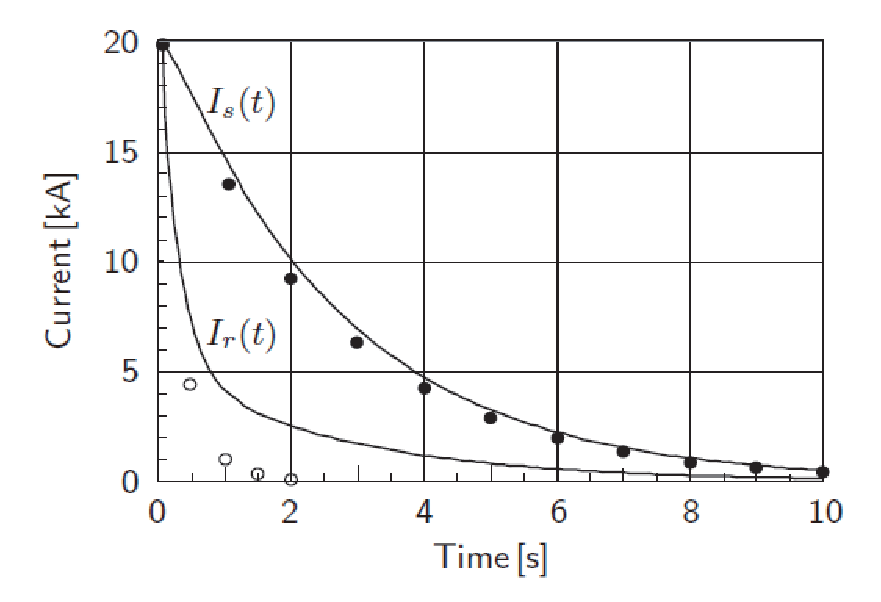
\includegraphics[scale=0.6]{chpt9/figs/fig9.3.eps}
	\caption{方程m.3两式在$M_{sr}=0$的曲线,实心点为$I_s(t)$,空心点为$I_r(t)$。各点列旁边的曲线是$M_{sr}$=0.017 H对应的解。}
\end{figure}

\textbf{n) 耦合效应}\qquad 两磁体显然是感性耦合的---$M_{sr}\neq 0$。
解释图9.3中,为什么$M_{sr}$=0.017 H对应的$I_s(t)$解在$M_{sr}=0$的实心点列上方。

\textbf{解:}我们可以把m.1的第一式写为
\begin{align*}% page552 第1个
L_s\frac{dI_s(t)}{dt}=-R_DI_s(t)-M_{sr}\frac{dI_r(t)}{dt} \tag{n.1}
\end{align*}
因为$dI_r(t)/dt<0$,方程n.1中的$-M_{sr}dI_r(t)/dt$为正,
从而令$|dI_r(t)/dt|$在$M_{sr}\neq 0$时要比在$M_{sr}=0$时小。
也即,$M_{sr}\neq 0$时的$I_s(t)$要比$M_{sr}=0$时衰减的更慢。
但是,因为$k_{sr}$并不很大,假定$M_{sr}=0$的快速解偏离并不大,至少对$I_s(t)$是如此。

\textbf{o) 有效衰减时间常数}\qquad 如上文n)中所述,当将两个磁体之间的电感耦合考虑进来后,
$I_s(t)$和$I_r(t)$相比m)中的不耦合系统衰减的更慢。
假设超导磁体在20 kA时储存的总磁能是55.4 MJ(按e)的计算)全部耗散于电阻$R_D$,
耦合系统中的$I_s(t)$使用``有效"时间常数$\tau_{eff}$表示,计算$\tau_{eff}$。

\textbf{解:}超导磁体的总磁能耗散于$R_D$,有:
\begin{align*}% page552 第2个
E_s=R_D\int_{0}^{\infty}I_s^2(t)dt \tag{o.1a}
\end{align*}
因为$I_s(t)=I_o e^{-t/\tau_{eff}}$,上式成为:
\begin{align*}% page552 第3个
E_s=R_D\int_{0}^{\infty}I_{o}^2e^{-2t/\tau_{eff}}dt=\frac{R_DI_o^2\tau_{eff}}{2} \tag{o.1b}
\end{align*}
解出上式的$\tau_{eff}$,有:
\begin{align*}% page552 第4个
\tau_{eff}=\frac{2E_s}{R_DI_o^2}=\frac{2(55.4\times10^6\ \mathrm{J})}{(0.1\ \mathrm{\Omega})(2\times10^4\ \mathrm{A})^2}=2.77\ \mathrm{s}
\end{align*}
可见,计算值比不耦合系统的计算值2.6 s略大$\sim6\%$。

\textbf{p) 磁滞损耗}\qquad 磁体从0到$B_m$励磁过程中,各超导丝中产生磁滞损耗。
估计一根直径为$d_f$=42 $\mu$m,位于CIC导体最内层之中的$\mathrm{Nb_3Sn}$细丝的空间平均磁滞能量密度$e_{hy1}$,
磁体缓慢通电流到20 kA,对应磁场为$B_m$=14 T。
从方程7.23a着手,该方程适用于存在传输电流下的Bean板(案例4i):
\begin{align*}% page553 第1个
e_{hy}=\frac{1}{2}\mu_oH_pH_m(1+i)^2\     \ [H_m\geq H_p(1-i)] \tag{7.23a}
\end{align*}
因为我们处理的导线假定为圆截面,直径为$d_f$,使用$H_p=(8/3\pi)J_c(d_f/2)$,该式
适用于垂直磁场下的导线(方程5.29b)。
接下来,因为$I_t$自0始,到20 kA止,远小于将近40 kA的$I_c$,令$(1+i)^2\simeq 1$可化简方程。
决定$H_p$的$J_c$在0和14 T之间宽幅变动。
也即,我们必须从$\mu_o H_m=B_m=0$到$B_m$=14 T对方程7.23a积分,
得到20 kA下最内层内的平均场:
\begin{align*}% page553 第2个
e_{hy1}\simeq\frac{2d_f}{3\pi}\int_{0}^{B_m}J_c(B,t,\epsilon)dB \tag{p.1}
\end{align*}
这里,$J_c(B,t,\epsilon)$是$\mathrm{Nb_3Sn}$的临界电流密度,其依赖性不仅考虑了B和T,还包括了
应力$\epsilon$。这是因为磁体在充磁和退磁过程中,作用于每一根导体丝上的应力是变化的。
对T的依赖也是很重要的,因为如果磁体充磁或退磁的过程不是足够缓慢从而导体可以在
可以忽略的温升下将热传给制冷剂,导体的温度降升高。
通常,p.1以闭式解积分将非常复杂。

不过,我们将在这里使用闭式解,通过:1) 以足够缓慢的速度改变磁场,维持导体温度为4.5 K;
2) 忽略应力对$J_c$的效应。对处于磁体中平面和最内层的$\mathrm{Nb_3Sn}$复合导体丝,我们可以使用
平均电流密度$\tilde{J}_c(B,4.5K0)$:
\begin{align*}% page553 第3个
\tilde{J}_c(B,4.5K,\epsilon=0)=\tilde{J}_c(0,4.5K)\frac{b_o}{b_o+B} \tag{p.2}
\end{align*}
式中,$\tilde{J}_c(0,4.5K)=42\times 10^9\ \mathrm{ A/m^2}$,
$b_o$=1 T。
方程p.2是$\mathrm{Nb_3Sn}$在4.5 K和$\epsilon=0$下的$\tilde{J}_c(B,T,\epsilon)$的粗略近似。

\textbf{解:}使用p.2,我们首先积分:
\begin{align*}% page553 第4个
\int_{0}^{B_m}\tilde{J}_c(B,4.5\ \mathrm{K})dB&=\tilde{J}(0,4.5\ \mathrm{K})b_o\int_{0}^{B_m}\frac{dB}{b_o+B}=\tilde{J}_c(0,4.5\ \mathrm{K})b_o\ln(\frac{b_o+B_m}{b_o})\\
&=(42\times10^9\ \mathrm{J/m^2})(1\ \mathrm{T})\ln15=113.7\times10^9\ \mathrm{J/m^4}
\end{align*}
将上式结果代入p.1,有:
\begin{align*}% page553 第6个
e_{hy1}\simeq\frac{2(42\times10^{-6}\ \mathrm{m})}{3\pi}(113.7\times10^9\ \mathrm{J/m^4})\simeq1014\ \mathrm{kJ/m^3}
\end{align*}
使用GRANDLF,Gavrilin根据p.1得到$e_{hy1}=1039\ \mathrm{kJ/m^3}$;
在我们的简化模型下,他得到$1122\ \mathrm{kJ/m^3}$---
该值略大因为$J_c(B,4.5\ \mathrm{K},\epsilon=0)>J_c(B,T>4.5\ \mathrm{K},\epsilon>0)$[9.2]。

\textbf{q) 充电速率 vs. 氦温升}\qquad 流体力学上看,该磁体的各层是并联的。
假定进入制冷工质的唯一热源是空间平均分布的磁滞损耗,计算磁体从0到20 kA
最大的恒电流充电速度$(dI_s/dt)_{mx}$,在该速度下,氦质量流量若为5 g/s,
氦的时间平均温升极限为$\Delta\tilde{T}_{he}\simeq 4.0$ K($=\tilde{T}_{cs}-T_{op}$)。
这里,$\tilde{T}_{cs}$是时间平均的电流分享温度,在$I_{op}$=0时,$T_{cs}$=10.3 K;
在$I_{op}$=20 kA时,$T_{cs}$=6.7 K:$\tilde{T}_{cs}$=8.5 K。
此处计算使用p)中在恒定温度下得到的$e_{hy}=1014\ \mathrm{kJ/m^3}$。

氦在4.5 K和3.5 atm下的物性如下:定压比热$C_{he}$=4.28 J/gK;
密度$\rho_{he}=0.132\ \mathrm{g/cm^3}$,且认为其在最内层与温度和压力无关。
首先,证明在最内层释放的磁滞损耗总能量$E_{hy1}$为3.5 kJ。

\textbf{解:}最内层释放的磁滞损耗总能量为:
\begin{align*}% page554 第1个
E_{hy1}=e_{hy}(A_{sc}+A_{\bar{m}})\ell_1
\end{align*}
式中,$(A_{sc}+A_{\bar{m}})=40.2\ \mathrm{ mm^2}$,$\ell_1$是最内层的导体总长度。
我们有$\ell_1\simeq 2\pi(a_1+w)(42)$,其中,$a_1$是绕组的内径,$w$是槽的径向深度,
42是每层的匝数---上述数据可从表9.1查得。
从图9.1和表9.1我们知道,磁体绕组的径向尺度$a_2-a_1$是305.1 mm,
包括18层CIC导体:$w$=(305.1 mm)/18$\simeq$17 mm。于是:
\begin{align*}% page554 第2个
\ell_1\simeq 2\pi(0.305\ \mathrm{m}+0.017\ \mathrm{m})42\simeq 85\ \mathrm{m}
\end{align*}
\begin{align*}% page554 第3个
E_{hy1}=(1014\times 10^3\ \mathrm{J/m^3})(40.2\times 10^{-6}\ \mathrm{m^2})(85\ \mathrm{m})\simeq 3.5\ \mathrm{kJ}
\end{align*}

在流量$\.{m}_{he}$=5 g/s下,氦的焓在最内层入口到出口的时间平均变化率$dH_{he}/dt$为:
\begin{align*}% page554 第4个
\frac{dH_{he}}{dt}&=C_{he}m_{he}\Delta\tilde{T}_{he}\\
&=(4.28\ \mathrm{J/gK})(5\ \mathrm{g/s})(4.0\ \mathrm{K})\simeq 86\ \mathrm{W}
\end{align*}
也即,在时间平均温升为4.0 K时,最内层的氦的冷却功率为86 W。
该冷却功率必须与最大耗散率$P_{{hy1}_{mx}}$相匹配:
\begin{align*}% page554 第5个
 P_{hy1_{mx}}\simeq\frac{E_{hy1}}{\Delta t_{mn}}=86\ \mathrm{W} \tag{q.1}
\end{align*}
在方程q.1中解出$\Delta t_{mn}$,我们得到:
\begin{align*}% page554 第7个
\Delta t{mn}=\frac{E_{hy1}}{P_{hy1_{mx}}}\simeq\frac{3.5\ \mathrm{kJ}}{86\ \mathrm{W}}\simeq 41\ \mathrm{s}
\end{align*}
于是:
\begin{align*}% page554 第8个
(\frac{dI_s}{dt})_{mx}=\frac{\Delta I_s}{\Delta t_{mn}}\simeq\frac{20\times 10^3\ \mathrm{A}}{41\ \mathrm{s}}\simeq 490\ \mathrm{A/s}
\end{align*}

这样,额定充电速度400 A/s可以保证导体低于其电流分享温度,该温度在$I_{op}=0$时
为10.3 K,在$I_{op}=20$ kA时为6.7 K。

\textbf{r) 耦合损耗}\qquad 使用方程7.36和7.39c (表7.8),计算耦合耗散能量密度$e_{cp}$。
计算条件为:导体细丝直径$D_{mf}$=0.6 mm,$\ell_p$=10 mm,
以很定充电速率400 A/s线性或$\tau_m$=50 s(如图7.18的三角形场激励)
将磁体由0充电至20 kA($B_m$=14 T)。
对于本Nb3Sn细丝,$\tau_{cp}$=30 ms[9.2]。

\textbf{解:}在$\tau_m\gg \tau_{cp}$下,三角波激励下的时间平均$e_{cp}$由7.36和7.39c的组合形式给出:
\begin{align*}% page555 第1个
e_{cp}=2\mu_oH_{m}^2[1+\frac{1}{4}(\frac{\pi D_{mf}}{\ell_p})^2]\Gamma \tag{7.36}
\end{align*}
\begin{align*}% page555 第2个
\Gamma\simeq\frac{4\tau_{cp}}{\tau_m}\   \  (\tau_m\gg \tau_{cp}) \tag{7.39c}
\end{align*}
方程7.36中,$(\pi D_{mf}/\ell_p)^2\ll 1$,$H_m=B_m/\mu_o$;
充电时间周期仅包括整个三角波的1/2(图7.18),
所以方程7.36中必须加入因子1/2。这样,$e_{cp}$成为:
\begin{align*}% page555 第3个
e_{cp}&\simeq\frac{1}{2}(2\frac{B_m^2}{\mu_o})\Gamma\\
&=\frac{4B_m^2\tau_{cp}}{\mu_o\tau_m} \tag{r.1}
\end{align*}

代入$B_m$=14 T,$\tau_{cp}$=30 ms以及$\tau_m$=50 s,我们得到:
\begin{align*}% page555 第5个
e_{cp}=\frac{4(14\ \mathrm{T})^2(30\times 10^{-3}\ \mathrm{s})}{(4\pi\times 10^{-7}\ \mathrm{T})(50\ \mathrm{s})}\simeq 357\ \mathrm{kJ/m^3}
\end{align*}

可见,耦合损耗约为磁滞损耗的$\sim 1/3$。

\textbf{s) 热点温度}\qquad 假定$t=0$时,超导磁体中检测到失超,断路器无时延打开---
即在$t=0$时刻打开。假定超导磁体中的电流$I_s(t)$以指数衰减,等效衰减常数$\tau_{eff}$=2.77 s
(如o)中所得)。同时假定初始失超点---``热点"---由焦耳热绝热加热。
计算热点的最终温度$T_f$。
同时假设,仅由CIC导体---超导体、非基底金属、基底(铜,RRR=100)---吸收焦耳热,
铜的热容量可用来代表全部导体的热容量。

\textbf{解:}根据方程8.16a,我们有:
\begin{align*}% page556 第1个
Z(T_f,T_i)=\left(\frac{A_m}{A_{cd}}\right)\int_{0}^{\infty}J_{m_o}^2e^{-2t/\tau_{dg}}dt=\left(\frac{A_m}{A_{cd}}\right)J_{m_o}^2\times\frac{1}{2}\tau_{dg} \tag{8.16a}
\end{align*}

将表9.1中的参数代入8.16a,$A_m=57.4\ \mathrm{mm^2}$;
$A_{cd}=A_m+A_{sc}+A_{\bar{m}}=97.6\ \mathrm{ mm^2}$;
$J_{m_{op}}=I_{op}/A_m=20000/57.4\times 10^{-6}=3.48\times 10^8\ \mathrm{ A/m^2}$;
将$\tau_{dg}=\tau_{eff}$=2.77 s代入s.1,解铜的$Z_{cu}(T_f,T_i)$,$Z(T_f,T_i)$:
\begin{align*}% page556 第2个
Z_{cu}(T_f,T_i)&=(\frac{57.4\times 10^{-6}\ \mathrm{m^2}}{97.6\times 10^{-6}\ \mathrm{m^2}})(3.48\times 10^8\ \mathrm{A/m^2})^2(\frac{2.77\ \mathrm{s}}{2})\\
&\simeq 9.9\times 10^{16}\ \mathrm{A^2s/m^4}
\end{align*}

从图8.2,我们找到$Z_{cu}(T_f,T_i=4.5\ \mathrm{K})=9.9\times 10^{16}\ \mathrm{A^2 s/m^4}$对应
铜(RRR=100)的$T_f\simeq 125$ K。

\textbf{t) 起始延时}\qquad 一个更贴近实际的场景应考虑从$t=0$热点出现到断路器实际打开的延时$\tau_{dl}$。
这是因为热点电压升高到触发断路器打开所需的水平需要一定时间。
假设这个期间$t_d$内,超导磁体的电流保持20 kA,估算热点最终温度$T_f$。除$\tau_{dl}$=0.5 s外,
条件假设同s)。

\textbf{解:}使用方程8.66b,并使用$\tau_{eff}$代替$\tau_{dg}$,有:
\begin{align*}% page557 第1个
Z(T_f,T_i)&=\left(\frac{A_m}{A_{cd}}\right)\left(\tau_{dl}+\frac{1}{2}\tau_{eff}\right)J_{m_{op}}^2\\
&\simeq 13.5\times 10^{16}\ \mathrm{A^2s/m^4}
\end{align*}

从图8.2,我们找到$Z_{cu}(T_f,T_i=4.5\ \mathrm{K})=13.5\times 10^{16}\ \mathrm{A^2 s/m^4}$
对应铜(RRR=100)的$T_f\simeq 225$ K,这几乎是可接受的热点温度的极限了。
尽管实际中由于制冷工质的冷却,$T_f$应能<225 K,但出于谨慎考虑,磁体产生热点后断路器应
确保在0.5 s内打开。
这意味着热点产生后,必须在远小于0.5 s的时间内将之检测到。

图9.4给出了温度(实线)和压力(虚线)与时间的关系图。该图由Gavrilin[9.2]制作,他使用GANDALF
计算了类似于s)的案例,他的计算中除了使用了$I_s(t)$的准确解,还考虑了氦的冷却效果和交流损耗。
大体上说,由于氦的冷却,热点温度$T_f$仅上升到$\sim$95 K,而不是s)中在绝热和$\tau_{dl}=0$
条件下计算的125 K。
分析还表明,通道内氦的压力峰值达到了23.5 atm。
\begin{figure}[htbp]
	\centering
	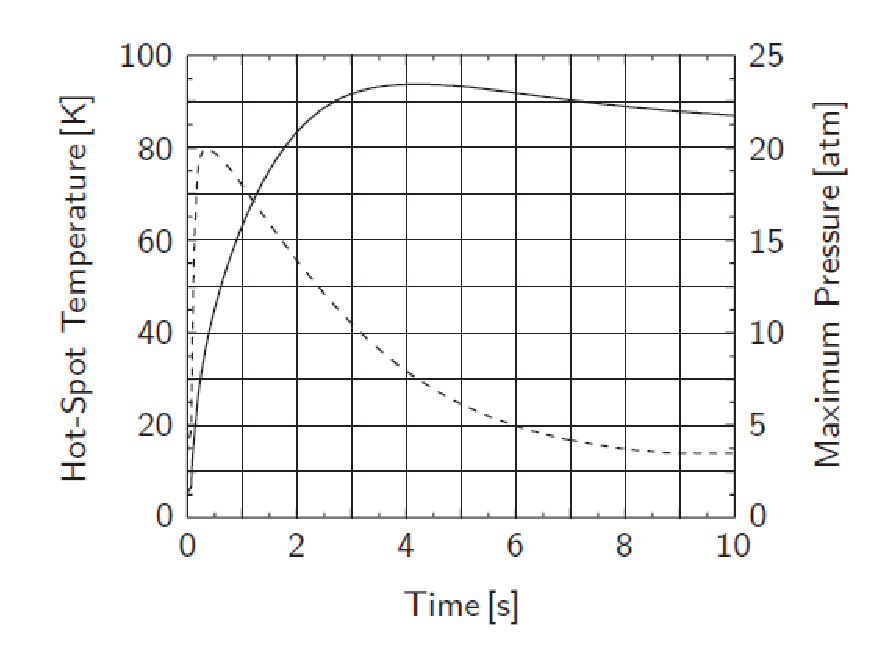
\includegraphics[scale=0.6]{chpt9/figs/fig9.4.eps}
	\caption{温度(实线,左y轴)和压力(虚线,右y轴)与时间的关系。}
\end{figure}


\begin{table}[htbp]\small
\centering
\caption{5个电阻内插线圈的参数}  
\begin{tabular}{|l|c|c|c|c|c|}
\hline
参数 & 线圈1 & 线圈2 & 线圈3 & 线圈4 & 线圈5 \\ \hline
\multirow{4}{*}{\begin{tabular}[c]{@{}l@{}}绕组内径i.d.($2a_1$) $\left[\mathrm{mm}\right]$\\ 绕组外径o.d.($2a_2$) $\left[\mathrm{mm}\right]$\\ 绕组高度($2_b$) $\left[\mathrm{mm}\right]$\\ 中心场$\left[\mathrm{T}\right]$\end{tabular}} & \multirow{4}{*}{\begin{tabular}[c]{@{}c@{}}54.0\\ 78.0\\ 239\\ 4.03\end{tabular}} & \multirow{4}{*}{\begin{tabular}[c]{@{}c@{}}80.4\\ 145.4\\ 238\\ 6.33\end{tabular}} & \multirow{4}{*}{\begin{tabular}[c]{@{}c@{}}151.4\\ 235.8\\ 317\\ 4.78\end{tabular}} & \multirow{4}{*}{\begin{tabular}[c]{@{}c@{}}241.8\\ 341.8\\ 353\\ 4.37\end{tabular}} & \multirow{4}{*}{\begin{tabular}[c]{@{}c@{}}347.8\\ 200.0\\ 605\\ 3.72\end{tabular}} \\
& & & & & \\
& & & & & \\
& & & & & \\ \hline
\end{tabular}
\end{table}


\textbf{u) 故障模式轴向力}\qquad SCH磁体的一个可能故障模式就在额定运行电流20 kA下,
5个电阻型插入线圈(图9.1)的各线圈的一半损坏(最恶劣情景)而形成电气短接,剩余一半继续工作产生磁场。
各线圈的上半部分短接时,各线圈的轴向场中心下移$b/2$;
对线圈5(最外侧),由图9.1可见,该值为$151\frac{1}{4}$ mm。
表9.2给出了5线圈电阻型插入磁体的关键参数[9.3]。

当这种情况发生后,超导磁体承受向下的轴向力,该力与电阻型磁体的承受向上力一致。
从图9.1我们可以看到,超导磁体承受的最大力来自线圈5,尽管其中心场是最小的。主要原因是:
1) 线圈5最大;2)它与超导磁体耦合最紧密。
参照下面给出的逐步的``简单"但``理由充分"的步骤,粗略计算线圈5和4对超导磁体的力。
这里的目标是让一个设计小组的非专家获得大致认知,组内的专家则会使用程序计算得到``精确"的数值。

3.5节,我们讨论了计算``简单"螺管线圈组合,特别是``环"线圈,薄壁线圈等的解析方法。
这些组合中,最简单的是两个环形线圈之间的力的计算(图3.5):
线圈A,直径$a_A$,总匝数$N_A$,电流$I_A$;线圈B,直径$a_B$,总匝数$N_B$,电流$I_B$。

\textbf{逐步过程}

过程包括两步。
\begin{description}
	\item[第一步] 将各线圈建模为环形线圈,使其产生和原始线圈相同的中心场。计算环形线圈在运行电流
	20 kA下的总匝数$N$。尽管超导磁体和电阻型线圈建模为薄壁螺管线圈更准确(图3.7),
	但相应的轴向力表达式更复杂,对评估大致情况显得不必要。
\item[第二步] 使用方程3.34计算两个环线圈之间的轴向力:首先是超导环线圈(线圈A)和电阻型环线圈5(线圈B)
之间的力;接下来计算超导环线圈(线圈A)和电阻型线圈4(线圈B)之间的力。
\end{description}

\textbf{两个环线圈之间的轴向力:复习}

对两个轴向距离$\rho$的环形线圈A和线圈B,两线圈之间的轴向力$F_{zA}(\rho)$为:
\begin{align*}% page559 第1个
F_{AZ}(\rho)=&\frac{\mu_o}{2}(N_AI_A)(N_BI_B)\frac{\rho\sqrt{(a_A+a_B)^2+\rho^2}}{(a_A-a_B)^2+\rho^2}\\
&\times\{k^2K(k)+(k^2-2)[K(k)-E(k)]\} \tag{3.34}
\end{align*}
$K(k)$和$E(k)$分别是第一类和第二类完全椭圆积分。
该系统椭圆积分的模量$k$为:
\begin{align*}% page559 第2个
k^2=\frac{4a_Aa_B}{(a_A+a_B)^2+\rho^2} \tag{3.36}
\end{align*}

\textbf{解:}使用方程3.111a给出的场表达式计算超导环形线圈A的匝数$N_A$:
\begin{align*}% page559 第3个
B_z(0,0)=\frac{\mu_oNI}{2a_1} \tag{3.111a}
\end{align*}
这里,$N=N_A,I=I_A, a_1=a_A$。
超导线圈的$a_A$的一个合适的值时平均绕组半径(表9.1):$a_A\simeq$458 mm。
于是,代入$B_Z(0,0)$=14.52 T和$I_A$=20 kA,我们有:
\begin{align*}% page559 第4个
N_A=\frac{2a_AB_Z(0,0)}{\mu_oI_A}=\frac{2(0.458\ \mathrm{m})(14.52\ \mathrm{T})}{(4\pi\times 10^{-7}\ \mathrm{H/m})(2\times 10^4\ \mathrm{A})}=529
\end{align*}

我们注意到$N_A$比磁体实际的匝数756小,这是由于产生相同的中心场,环形线圈要比
各匝分布于很大的绕组截面上的实际磁体效率高。

将线圈5建模为环形线圈B需要更加的小心:中心场3.72 T不能直接使用,因为这是线圈5在故障前
产生的中心场。现在,轴向距离$2b$折半了,于是,我们必须首先计算线圈5在$\beta'=\beta/2$
时产生的中心场。
对于Bitter磁体,场因子$[F(\alpha,\beta)]_B$由方程3.115b给出:
\begin{align*}% page559 第5个
[F(\alpha,\beta)]_B=\ln\left(\alpha\frac{\beta+\sqrt{1+\beta^2}}{\beta+\sqrt{\alpha^2+\beta^2}}\right) \tag{3.115b}
\end{align*}

因为损坏线圈中的``健康"的一半线圈的参数不变,新的中心场$[B_Z'(0,0)]_B$
可以由原中心场$[B_Z(0,0)]_B$给出:
\begin{align*}% page559 第6个
\frac{[B_Z'(0,0)]_B}{[B_Z(0,0)]_B}
=\frac{[F(\alpha,\beta')]_B}{[F(\alpha,\beta)]_B}
=\frac{\ln(\alpha\frac{\beta'+\sqrt{1+\beta'^2}}{\beta'+\sqrt{\alpha^2+\beta'2}})}{\ln(\alpha\frac{\beta+\sqrt{1+\beta^2}}{\beta+\sqrt{\alpha^2+\beta^2}})} \tag{u.1}
\end{align*}

将线圈5的以下值代入方程u.1:$[B_z(0,0)]_B=3.72$ T,$\alpha\simeq$1.44(=500.0 mm/347.8 mm),
$\beta\simeq$1.74(=605 mm/347.8 mm),$\beta'=\beta/2\simeq$1.74/2=0.87。
解出$[B'_z(0,0)]_B$,我们得$[B'_z(0,0)]_B$=2.66 T。

线圈5'的$a_B$一个合理值是其几何平均值$a_B=\sqrt{a_1 a_2}$=208.5 mm而不是算术平均值
$(a_1+a_2)/2$=212.0 mm。这是因为Bitter线圈中电流密度是不均匀的,而是随$\propto 1/r$变动(方程3.114)。
为了简化,我们取$a_B$=174 mm。这样,代入$[B'_z(0,0)]_B$=2.66 T和$I_B=$20 kA:
\begin{align*}% page560 第1个
N_B=\frac{2(0.174\ \mathrm{m})(2.66\ \mathrm{T})}{(4\pi\times 10^{-7}\ \mathrm{H/m})(2\times 10^4\ \mathrm{A})}\simeq 37
\end{align*}
代入$a_A$=0.458 m,$a_B$=0.174 m,$a_A+a_B$=0.632 m和$\rho=$0.151 m(线圈5原始值的1/4),
首先计算出模量$k$:
\begin{align*}% page560 第2个
k^2&=\frac{4a_Aa_B}{(a_A+a_B)^2+\rho^2}\\ \tag{3.36}
&=\frac{4(0.458\ \mathrm{m})(0.174\ \mathrm{m})}{(0.632\ \mathrm{m})^2+(0.151\ \mathrm{m})^2}\\
&\simeq 0.7550\ \ (k\simeq 0.8689)
\end{align*}
向方程3.34中代入$K(0.8689)=2.1655, E(0.8689)=1.2079, a_A-a_B=0.284$ m和其他参数,
我们得到线圈B(线圈5的一半)施于线圈A(超导磁体)的力$F_{zA}(\rho=151\ \mathrm{mm})$为:
\begin{align*}% page560 第5个
F_{zA}(151\ \mathrm{mm})=&\frac{4\pi\times10^{-7}\ \mathrm{H/m}}{2}(529)(2\times 10^4\ \mathrm{A})(37)(2\times 10^4\ \mathrm{A})\\
&\times[\frac{(0.151\ \mathrm{m}\sqrt{(0.632\ \mathrm{m})^2+(0.151 \ \mathrm{m})^2})}{(0.284\ \mathrm{m})^2+(0.151\ \mathrm{m})^2}\\
&\times\{0.7550(2.1655)+(0.7550-2)(2.1655-1.2079)\}]\\
=&(4.92\ \mathrm{MN})\times[0.948\times 0.443]=2.06\ \mathrm{MN}
\end{align*}

为了计算线圈B(线圈4的一半)施于线圈A的力,我们有线圈B的以下新参数:
$\alpha=1.41;\beta=1.46;\beta'=0.73;B'_z(0,0)$=2.96 T;$N_B\simeq 28; a_B=0.121$ m。
代入$\rho$=0.088 m; $a_A+a_B$=0.579 m; $a_A-a_B$=0.337 m,我们有:
$k^2\simeq 0.6463(k\simeq 0.8039)$,对应给出的$K(0.8039)\simeq 2.0030, E(0.8039)\simeq 1.2728$。
将这些值代入方程3.34,我们得到$F_{zA}(88\ \mathrm{mm})=0.49$ MN。
该值比线圈5初始所施的力的1/4,意味着线圈1-3的贡献可以忽略。

采用程序计算的线圈1-5的合力是1.9 MN[9.3]。
我们的基于简化模型的方法需要用计算器按上一段时间,最终给出的结果似乎2.06 MN(仅来自线圈5),
这个值作为估算来讲已经够好。

\textbf{磁场屏蔽}

因为磁体越大(尺寸、场强或两者都大),它的边缘场延伸的范围越大,故``大"磁体通常需要屏蔽。
主动屏蔽使用电磁体(屏蔽线圈);被动屏蔽使用铁磁结构(钢壳)。
主动屏蔽为保证其他设计参数,应离主磁体尽可能的远,因为它会弱化磁场;
被动屏蔽通常增加磁场。
高场(>1 T)MRI和多数NMR磁体如今都是主动屏蔽、被动屏蔽或两者兼容屏蔽的。

如开始所述,SCH磁体与实验所用空间相邻。为了减少磁体对旁边的实验的磁场干扰,
SCH磁体系统需要一个屏蔽线圈,如图9.5 SCH磁体截面示意图的右侧所示。
有一个很大的室温孔的电阻性磁体,相比超导主磁体来说贡献了很小的边缘场,在图中忽略未画出。
图9.5的左侧给出了一个钢壳,用于被动屏蔽---这是屏蔽超导主磁体的另一种方法。

如图9.5所示,主动屏蔽线圈(本磁体首创[9.1])实际上是由两个子线圈构成,一个放置在中平面上方,另一个在下方;
这里两个子线圈都被建模为环形线圈。
钢壳是圆柱形的,在这里的分析中被建模为周向将主磁体完全围住。两个元件的重要方面此处都将进行研究。

\begin{figure}[htbp]
	\centering
	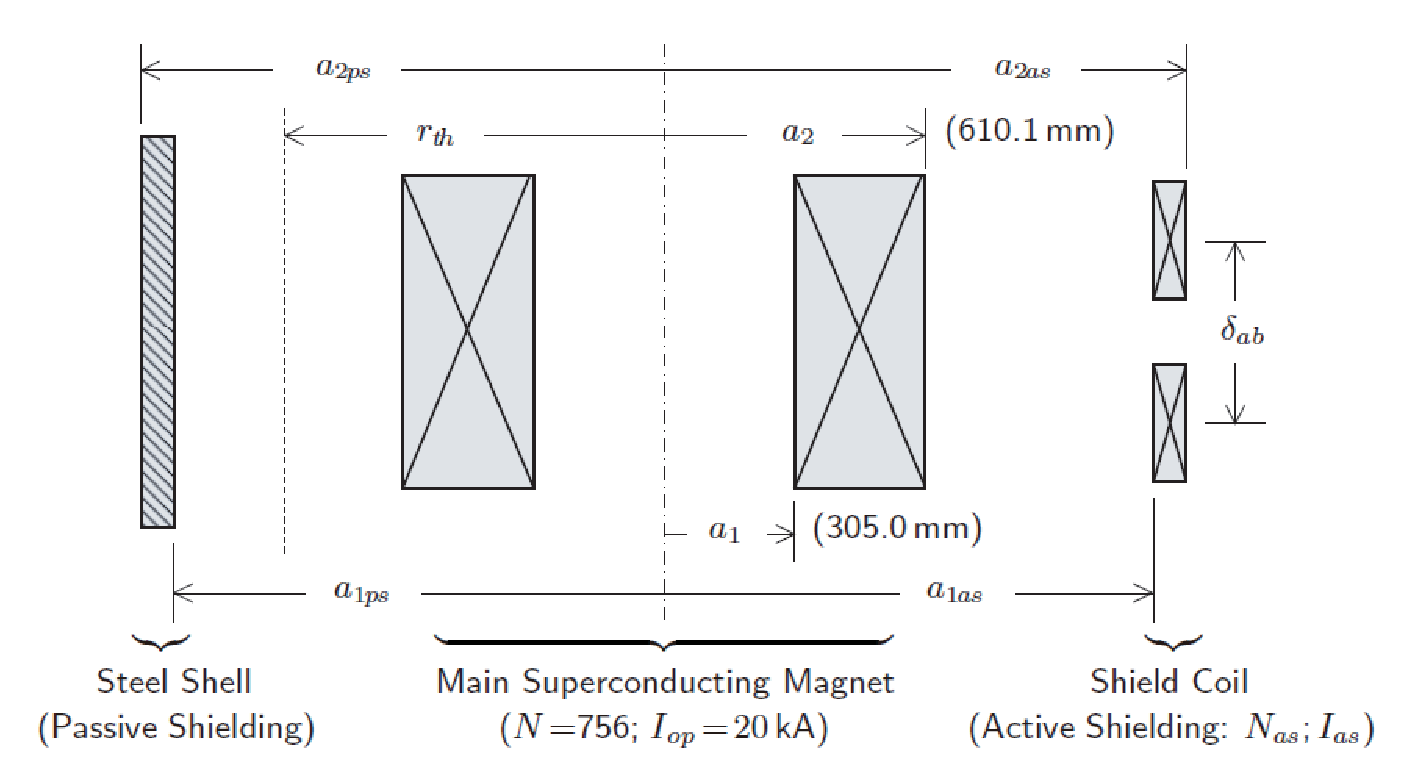
\includegraphics[scale=0.6]{chpt9/figs/fig9.5.eps}
	\caption{主磁体使用屏蔽线圈(主动屏蔽)或钢壳9(被动屏蔽)的截面图。主动屏蔽线圈由两个子线圈组成,分别在
		中平面的上方和下方。}
\end{figure}

\textbf{v) 主动屏蔽线圈---匝数}\qquad 将两个用于磁屏蔽的子线圈建模为\textit{单}屏蔽线圈。
然后,将超导主磁体线圈和上述屏蔽线圈转换为偶极子。
现在,估算这个模型屏蔽线圈的总匝数,令其磁极矩与主磁体的极矩匹配。
屏蔽线圈和运行于20 kA的主磁体串联,但极性相反。

\textbf{解:} 远离螺管磁体中心的磁场$\vec{H}_f$可以建模为偶极子(问题3.1):
\begin{align*}% page562 第1个
\vec{H}_f=H_0\left(\frac{R_e}{r}\right)^3\left(\cos\theta{\vec{\imath}_r}+\frac{1}{2}\sin\theta\vec{\imath}_\theta\right) \tag{3.163}
\end{align*}
$R_e$是偶极子的半径。
对一个安匝$NI$均匀分布的螺管,乘积$H_0 R_e^3$由下式给出:
\begin{align*}% page562 第2个
H_0R_e^3=\frac{1}{6}(a_1^2+a_2^2+a_1a_2)NI \tag{3.165}
\end{align*}
式中,$a_1$和$a_2$分别是磁体绕组的内外半径。
因为$\vec{H}_f\propto (R_e/r)^3$以及$H_0 R_e^3\propto a_1^2$,
这里,我们实际上可以忽略电阻性插入磁体---线圈5的$a_1$=173.9 mm,
超导磁体的$a_1$=305.0 mm。
对主超导磁体和屏蔽线圈(下标$as$)分别应用方程3.163和3.165,有:
\begin{align*}% page562 第3个
a_1^2(1+\alpha^2+\alpha)NI_{op}=a_{1as}^2(1+\alpha_{as}^2+\alpha_{as})N_{as}I_{as} \tag{v.1}
\end{align*}
其中,$\alpha_{as}=a_{2as}/a_{1as}$。代入$I_{as}=I_{op}$,从v.1中解出$N_{as}$:
\begin{align*}% page562 第4个
N_{as}=(\frac{a_1}{a_{1as}})^2(\frac{1+\alpha^2+\alpha}{1+\alpha_{as}^2+\alpha_{as}})N \tag{v.2}
\end{align*}
将$a_1$=0.305 m,$a_{1as}$=1.203 m,$\alpha=2.00$,$\alpha_{as}$=1.04和$N$=756代入
v.2,$N_{as}$成为:
\begin{align*}% page562 第5个
N_{as}=(\frac{0.305\ \mathrm{m}}{1.203\ \mathrm{m}})^2(\frac{1+4+2}{1+0.8+1.04})(756)\simeq 109
\end{align*}

屏蔽线圈的实际匝数似乎78[9.4],并且是由两个如图9.5所示的子线圈组成的。
轴向绕匝的位移未引起磁矩衰减;若匝数轴向展开,仅磁场降低。

\textbf{w) 主动屏蔽线圈对中心场的减弱}\qquad 前文提及,主动屏蔽线圈产生于超导主磁体反向的磁场。
计算主动屏蔽线圈在中心的轴向场$B_z^{as}(0,0)$。
屏蔽线圈使用以下参数:$a_{1as}$=1.203 m;$a_{2as}$=1.250 m;
$b_{as}$=0.471 m(实际系统中,主动屏蔽线圈由两个稍短的子线圈构成,两者各据中平面有一个间隙[9.4]);
$N_{as}$=78;和$I_{as}$=20 kA。

\textbf{解:}磁场的计算是方程3.110的直接应用:
\begin{align*}% page563 第1个
B_z(0,0)=\frac{\mu_oNI}{2a_1(\alpha-1)}\ln(\frac{\alpha+\sqrt{\alpha^2+\beta^2}}{1+\sqrt{1+\beta}}) \tag{3.110}
\end{align*}
代入$N\rightarrow N_{as}=78$,$I\rightarrow I_{as}$=20 kA,$\alpha\rightarrow \alpha_{as}$=1.04,
$\beta\rightarrow \beta_{as}=0.392$以及$a_1\rightarrow a_{1as}=1.203$,
$B_z^{as}(0,0)$成为:
\begin{align*}% page563 第2个
B_z^{as}(0,0)&=\frac{(4\pi\times 10^{-7}\ \mathrm{H/m})(78)(20\times 10^3\ \mathrm{A})}{(2.406\ \mathrm{m})(1.04-1)}\ln(\frac{1.04+\sqrt{(1.04)^2+(0.392)^2}}{1+\sqrt{1_(0.92)^2}})
&\simeq 0.75\ \mathrm{T}
\end{align*}

因为若无主动屏蔽线圈,20 kA的超导主磁体的中心场是14.52 T(Q/A 9.1的问题b)计算所得),
主动线圈将之降低了0.75 T,约为5\%。总的来看,已经不能忽视。

\textbf{x1) 主动屏蔽线圈---作用力:1}\qquad 如果屏蔽线圈建模为单线圈,那么它和主磁体之间不会有
净作用力。在原始系统中,屏蔽线圈被分为两个子线圈。
此时,作为整体的屏蔽线圈和主磁体之间仍无净作用力,
但是各子线圈与主磁体之间均存在作用力。
这里我们将主磁体和其中一个子线圈均建模为``环线圈",计算其作用力的大致幅值。
取$\rho$=0.227 m(中心对中心距离)。
由于图9.5中的$\delta_{ab}=2\rho$,$\delta_{ab}$=0.554 m。

\textbf{解:}在前文t)中,主磁体已被建模为环形线圈:$N_A$=529;$a_A\simeq$458 mm。
类似的,我们可以将其中的一个子线圈建模为环线圈,使其产生中心场0.375 T(0.75 T的一半,
尽管两者是垂直放置的):
$a_B$=1.227 m($a_{1as}$和$a_{2as}$的平均值),$N_B$为:
\begin{align*}% page563 第3个
N_B\simeq\frac{(0.375\ \mathrm{T})2(1.227\ \mathrm{})}{(4\pi\times 10^{-7}\ \mathrm{H/m})(20\times 10^3\ \mathrm{A})}\simeq 37
\end{align*}

由于各子线圈的$\alpha=1.04$和很小的$\beta$表明它们非常接近环形线圈($\alpha=1,\beta=0$),
所以``有效匝数"37与实际匝数39如此接近并不令人惊讶。
首先,我们使用t)节用到的方程3.36计算模量常数$k$:
\begin{align*}% page563 第4个
k^2&=\frac{4a_Aa_B}{(a_A+a_B)^2+\rho^2}\\ \tag{3.36}
&=\frac{4(0.458\ \mathrm{m})(1.227\ \mathrm{m})}{(0.458\ \mathrm{m+1.227\ \mathrm{m}})^2+(0.227\ \mathrm{m})^2}\simeq 0.7709\   \ (k\simeq 0.8780)
\end{align*}

两个环线圈之间的作用力由3.34给出:
\begin{align*}% page564 第1个
F_{ZA}(\rho)=&\frac{\mu_o}{2}(N_AI_A)(N_BI_B)\frac{\rho\sqrt{(a_A+a_B)^2+\rho^2}}{(a_A-a_B)^2+\rho^2}\\
&\times\{k^2K(k)+(k^2-2)[K(k)-E(k)]\} \tag{3.34}
\end{align*}
代入$K(0.8780)=2.1957,E(0.8780)=1.1977,a_A+a_B=$1.685 m, $a_A-a_B=-0.769$ m,
我们得到线圈B(上方子线圈)对线圈A(主磁体)的力$F_{ZA}(\rho=0.227\ \mathrm{m})$:
\begin{align*}% page564 第2个
F_{ZA}(0.277\ \mathrm{m})=&\frac{4\pi\times 10^{-7}\ \mathrm{H/m}}{2}(529)(2\times 10^4\  \mathrm{A})(37)(-2\times 10^{4}\ \mathrm{A})\\
&\times \big[\frac{(0.277\ \mathrm{m})\sqrt{(1.685\ \mathrm{m})^2+(0.277\ \mathrm{m}^2)}}{(-0.769\ \mathrm{m})^2+(0.277\ \mathrm{m})^2}\\
&\times\{0.7709(2.1957)+(0.7709-2)(2.1957-1.1977)\}\big]\\
=&-(4.91\ \mathrm{MN})\times(0.7080\times 0.4660)=-1.62\ \mathrm{MN}
\end{align*}

作用在主磁体上的力是负值(向下);同样大小的力作用在中平面上方的屏蔽子线圈,向上;也即,
如果线圈没有约束,它将被推离中平面。
当然,上下两个子线圈对主磁体的合力为零。

\textbf{x2) 主动屏蔽线圈---作用力:2}\qquad 这里我们计算两个子线圈之间的引力。将两个线圈建模为
相同的环形线圈,直径1.227 m,匝数37,电流-20 kA。这里$\rho$=0.554 m,等于图9.5中的$\delta_{ab}$。

\textbf{解:}因为环形线圈直径相同($a$),尽管在这里条件$\rho(=0.554)\ll 2a(=2.454)$并不严格满足,
我们仍使用方程3.34在$\rho\ll 2a$条件下的简化版本3.39d。本例中,$N_B I_B=N_A I_A$:
\begin{align*}% page564 第3个
F_{ZA}(\rho)&\simeq\mu_o(N_AI_A)(N_BI_B)(\frac{a}{\rho})\\ \tag{3.39d}
&=\mu_o(N_AI_A)^2(\frac{a}{\rho})\\
&=(4\pi10^{-7}\ \mathrm{H/m})[(37)(-2\times 10^4\ \mathrm{A})]^2(\frac{1.227\ \mathrm{m}}{0.554\ \mathrm{m}})\\
&\simeq 1.5\ \mathrm{MN}
\end{align*}

这和用程序[9.3]计算得到的1.6 MN非常吻合。

\textbf{y1) 被动屏蔽壳:1}\qquad 除主动屏蔽外,还可以采用被动屏蔽。被动屏蔽使用铁磁材料,通常
是软铁(见问题2.3和表2.5)来实现。
被动屏蔽的优势主要是费用低,但对于``大型"和``高场"磁体,费用优势就没有了。
另一个经常被忽视的优势是它的``逆向屏蔽"能力,即它还能屏蔽相邻磁体的外围磁场对主磁体的影响。
笨重是被动屏蔽的最大劣势。

这里,我们考虑一个钢制圆柱筒,内半径$a_1\equiv a_{1as}=1.203$ m,高$2b_s=2a_{1as}$(图9.5)。
假定主磁体($N=756;I_{op}$=20 kA)可以建模为偶极矩,其$B_0R_e^3$由方程v.1给出(忽略电阻内插磁体),
估算圆柱筒的外半径$a_{2as}$,使其壁厚度足够保证刚的磁化$\mu_o M_s$在1.25 T时仍有较高的值
$(\mu/\mu_o)_{dif}:(\mu/\mu_o)_{dif}=180$(表2.5中的as-cast钢)。

\textbf{解:}$(\mu/\mu_o)_{dif}=180$时,我们可以将之视为理想的$(\mu/\mu_o)_{dif}=\infty$。
由于主磁体的所有磁通都从磁体室温孔发出,位于$r\ge a_{1as}$的磁通将在上方穿入钢制圆柱筒,并在其下方穿出
返回磁体室温孔。
稍微复杂的是磁体外半径$a_2\simeq0.610$ m与钢制圆柱筒内半径$a_{1ps}=1.203$ m之间的环形空间的磁通线。

因钢的磁阻小于空气,磁通线选择通过钢。这样,$r=a_2$之外的磁通线要么直接垂直进入空气
经$b=0.471$ m到达中平面(表9.1),要么首先径向走过距离$a_{1ps}-a_2=0.593$ m达到钢制
圆柱筒上方,而后垂直``无阻"的进入钢内到达中平面。因为0.471 m<0.593 m,
所以这些磁通不会进入钢内。
根据这个判断,我们可以给出一个半径的阈值$r_{th}$,超过该值,磁通线将改路进入钢圆柱筒内,
该值大概是$a_{1ps}-b=0.732$ m。也即,所有的位于$r_{th}$ m到$r=\infty$之间的磁通线
将进入钢制圆柱筒。于是,中平面上在$r_{th}$ m到$\infty$的总磁通$\Phi(r_{th/\infty,z=0})$和中平面上
通过钢的磁通$\Phi_s(z=0)$分别由下式给出,其中$\alpha=a_2/a_1$:
\begin{align*}% page565 第1个
\Phi(r_{th}/\infty,z=0)=\frac{1}{2}[\frac{\mu_oa_1^2(1+\alpha^2+\alpha)NII_{op}}{6}]\int_{r_{th}}^{\infty}\frac{2\pi r}{r^3}dr \tag{y1.1a}
\end{align*}
\begin{align*}
\Phi_{z}(z=0)=\pi(a_{2ps}^2-a_{1ps}^2)(\mu_oM_s) \tag{y1.1b}
\end{align*}
因为上述两个磁通相等,我们有:
\begin{align*}% page565 第3个
\frac{\mu_oa_1^2(1+\alpha^2+\alpha)NI_{op}}{6r_{th}}=(a_{2ps}^2-a_{1ps}^2)(\mu_oM_s) \tag{y1.2}
\end{align*}
在上式中解出$a_{2ps}$,我们得到:
\begin{align*}% page565 第4个
a_{2ps}=\sqrt{a_{1ps}^2+\frac{\mu_oa_1^2(1+\alpha^2+\alpha)NI_{op}}{6r_{th}(\mu_oM_s)}} \tag{y1.3}
\end{align*}
向y1.3中代入合适的值,计算得:
\begin{align*}% page566 第1个
a_{2ps}&=\sqrt{(1.203\ \mathrm{m})^2+\frac{(4\pi\times 10^{-7}\ \mathrm{H/m})(0.305\ \mathrm{m})^2(7)(756)(20\times 10^3\ \mathrm{A})}{6(0.732\ \mathrm{m})(1.25\ \mathrm{T})}}\\
&=\sqrt{1.447\ \mathrm{m^2}+2.254\ \mathrm{m^2}}=1.942
\end{align*}

钢制圆柱筒的壁厚$a_{2ps}-a_{1ps}$于是为72 cm。
这样的一个高为2.4 m的圆柱筒总重量约为133000 kg,超过100吨。

因为钢圆柱筒内的磁场主要是轴向($z$)的,同时切向场(这里为$z$向)必须在钢-空气边界连续,
所以,磁场可由$\sim \mu_o M_s/(\mu/\mu_o)_{dif}$给出,即
在$r=a_{1ps}$=1.203 m处和$r=a_{2ps}$=1.924 m处有1.25 T/180=0.0069 T或69 gauss;
在$r\simeq 20$ m处,磁场衰落至小于1 gauss。
根据法向(轴)的磁通连续性,钢圆柱筒内的向下的1.25 T磁通在``回到"磁体中平面后方向变为向上,
增强主超导磁体产生的14.52 T磁场。
从这个意义上,被动屏蔽要优于主动屏蔽。

\textbf{y2) 被动屏蔽壳:2}\qquad 很明显,钢圆柱壳放置的离主磁体越远,对壳壁厚的要求越薄,
这在方程y1.3可明显看出。
不过,根据被动屏蔽的基本规律,为了消除一个给定的偶极矩,
如果钢被极化到同一水平,所需的钢量与钢屏蔽体所处位置无关。
这里,考虑一个比壳1大50\%的$a_{1ps}=1.805$ m(3.6 m高)的壳2,计算$a_{2ps}$,
核验壳2的质量是否仍为133000 kg。

\textbf{解:}使用和上文相同的依据,我们得到磁通线的新的阈值半径$r_{th}=a_{1ps}-b$=1.805 m
-0.471 m=1.334 m。
向方程w.3中代入合适的参数值,计算有:
\begin{align*}% page566 第2个
a_{2ps}&=\sqrt{(1.805\ \mathrm{m})^2+\frac{(4\pi\times 10^{-7}\ \mathrm{H/m})(0.305\ \mathrm{m})^2(7)(756)(20\times 10^3\ \mathrm{A})}{6(1.334\ \mathrm{m})(1.25\ \mathrm{T})}}\\
&=\sqrt{3.258\ \mathrm{m^2}+1.237\ \mathrm{m^2}}=2.120\ \mathrm{m}
\end{align*}

圆柱壳的厚度$a_{2ps}-a_{1ps}$这时成为32 cm,比壳1薄了一半,
导致壳2的总质量为109000 kg,比壳1轻。
上述差异表明这个简单的分析方法仅对于估计钢屏蔽的大概值是有效的。


\subsection{例B:钢板上的超导线圈}
在这个螺管磁体系统案例中,我们应用铁磁球体对场屏蔽(问题2.3)和理想偶极子中的铁扼效应(问题3.8)
中用到的基本规律来研究圆形钢板如何影响置于其上的超导线圈的磁场。
我们将看到,钢板显著增强了上方的磁场,且几乎消除了钢板下的磁场。
在场屏蔽和偶极磁体的案例中,钢同样被建模为理想铁磁材料,即$\mu/\mu_o=\infty$。

图9.6给出了置于大直径、厚为$\delta_{st}$的圆形钢板上的超导磁体的截面图。
$z-r$坐标的中心与线圈中心重合。图中线圈未画出其骨架。
表9.3列出了线圈的参数。

图9.7画出了线圈通流25 A且无钢板时在$z$=0,5,7.5,10,12.5,15,17.5和20 mm时的$B_z(z,r)$。

\begin{table}[htbp]\small
\centering
\caption{线圈参数}  
\begin{tabular}{|l|c|}
\hline
参数 & 数值 \\ \hline
绕组内径i.d.($2a_1$) $\left[\mathrm{mm}\right]$ & 40 \\ \hline
绕组外经o.d.($2a_2$) $\left[\mathrm{mm}\right]$ & 70 \\ \hline
绕组高度($2_b$) $\left[\mathrm{mm}\right]$ & 10 \\ \hline
总匝数(N) & 150 \\ \hline
\end{tabular}
\end{table}



\begin{figure}
	\centering
	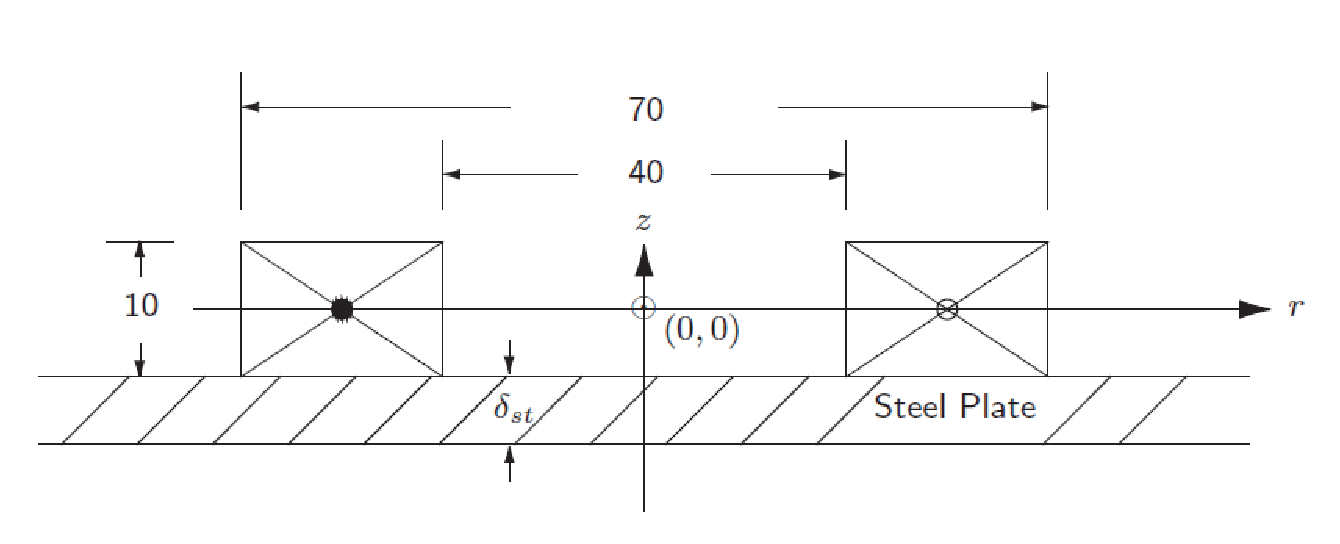
\includegraphics[scale=0.5]{chpt9/figs/fig9.6.eps}
	\caption{置于钢板上的超导线圈的截面图。尺寸单位为mm。}
\end{figure}


\begin{figure}
	\centering
	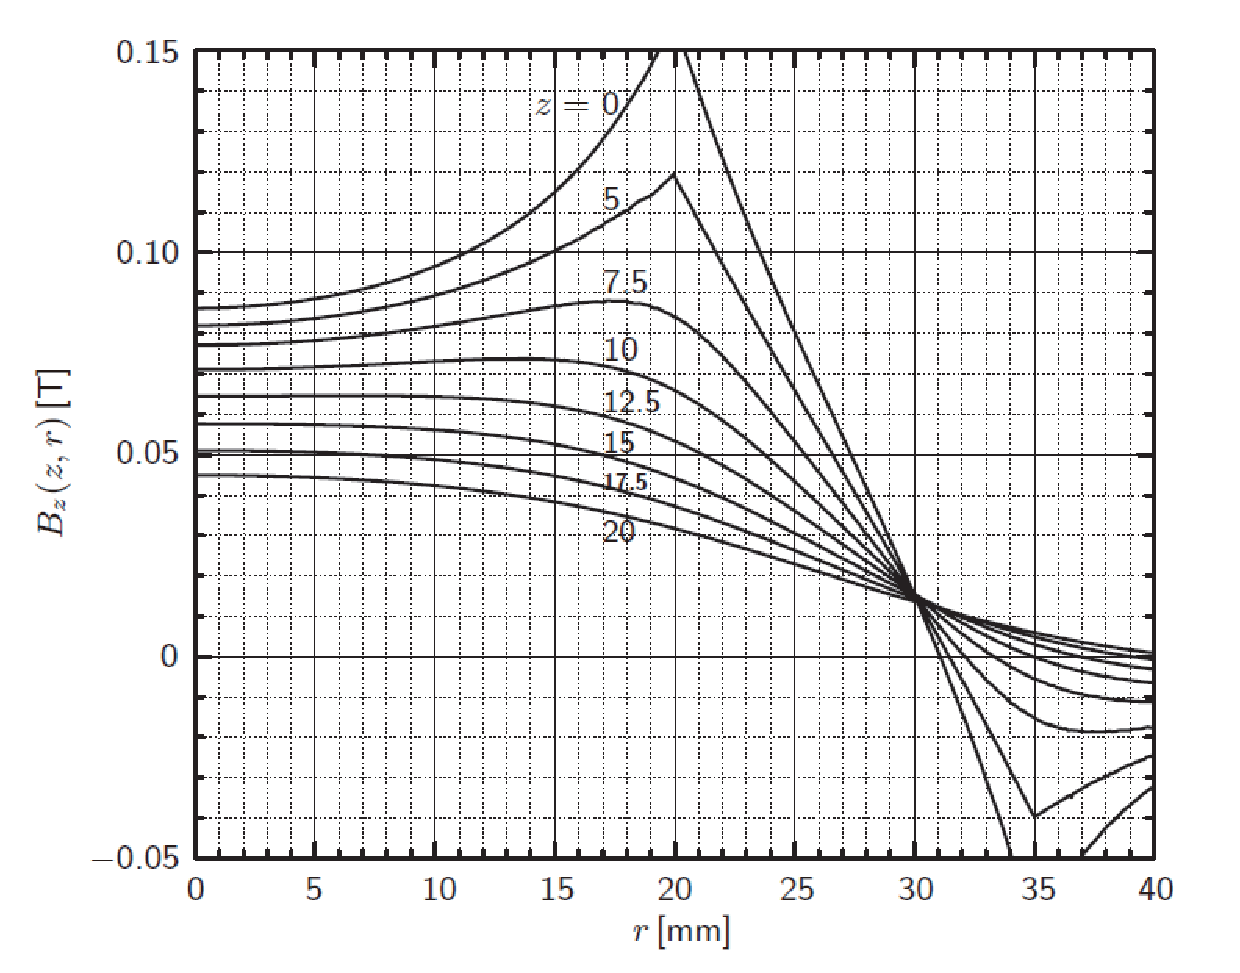
\includegraphics[scale=0.5]{chpt9/figs/fig9.7.eps}
	\caption{线圈通流25 A且无钢板时在$z$=0,5,7.5,10,12.5,15,17.5和20 mm时产生的磁场$B_z(z,r)$。
		$B_z(0,20)$=0.158 T,$B_z(0,35)$=-0.068 T。}
\end{figure}

\textbf{电感回顾}

如3.7节所讨论的,线圈的自感$L$可以由$\Phi$和$I$的关系给出:
\begin{align*}% page568 第1个
\Phi=LI \tag{3.78}
\end{align*}
其中$\Phi$是电流$I$时的总磁链:
\begin{align*}% page568 第2个
\Phi=2\pi\sum_{j=1}^{N}\int_{0}^{R_j}rB_z(z_i,r)dr \tag{9.1}
\end{align*}
式中,$R_j$是轴向距离$z=z_j$处的第$j$匝的半径。
明显这个积分手算起来很麻烦。但如今因为有了大量可以计算电感的程序,手算已不再必要。

这里我们针对图9.6所给的线圈,通过联立方程3.78和方程9.1的简化版本来计算电感的``说得过去精确"的值。
\begin{align*}% page568 第3个
L\simeq\frac{2N\pi}{I}\int_{0}^{a_2}B_z(z=0,r)dr \tag{9.2}
\end{align*}
方程9.2中,9.1的被积函数由一个仅涉及线圈中平面磁场的简单积积分项$B_z(0,r)$近似。
方程9.2给出了$L$的上限,因为并非所有$N$匝都在$r=a_2$交链;
实际上一些磁通仅交链于$a_1$内。
或许中间点$(a_1+a_2)/2$是径向积分限的一个很好的折中。


\subsubsection{Q/A B:钢板上的超导线圈}
\textbf{a) 线圈电感}\qquad 使用方程9.2和图9.7的$B_z(0,r)$图,计算线圈自感(无钢板)。
使用$B_z(0,r=20)$=0.158 T和$B_z(0,r=35)=-0.068$ T。

\textbf{解:}首先,$B_z(0,r)$和$B_z(0,r)r$的数据已列于表9.4。图9.8给出了$B_z(0,r)r$ vs. $r$曲线,
从中可知$\int B_z(0,r)rdr$和$\Phi$可以如下计算:
\begin{align*}% page569 第1个
\int_{0}^{a_2}B_z(0,r)dr&\simeq 38.0\ \mathrm{T mm^2}\mbox{图9.8中阴影部分}\\
&=3.80\times 10^{-5}\ \mathrm{Tm^2}\\
\Phi&=2\pi(3.80\times 10^{-5}\ \mathrm{Tm^2})\simeq 23.9\times 10^{-5}\ \mathrm{Tm^2}
\end{align*}
于是,
\begin{align*}% page569 第2个
L=\frac{N\Phi}{I}\simeq\frac{150(23.9\times 10^{-5}\ \mathrm{Tm^2})}{25\ \mathrm{A}}\simeq 1.43\ \mathrm{mH}
\end{align*}
该值比实际值1.33 mH大$\sim 10\%$。
由于在$-5\le z\le 5$ mm范围内,$B_z(0,r)$要比$B_z(z,r)$的平均值大,故方程9.2高估了$L$。
注意到,因为$B_z(0,r)r$在$r\simeq31$ mm和$a_2$之间积分为负,并且它与$(a_1+a_2)/2=27.5$ mm到
31 mm之间的积分制很接近,所以从0到$a_2$的积分最终与从0到$(a_1+a_2)/2$(上文提出的
更合适的积分限)之间的积分值近乎相等。

如3.7.2部分讨论的,对于一个参数为$a_1,\alpha,\beta,N$的螺管,其自感可由下式计算:
\begin{align*}% page569 第3个
L=\mu_oa_1N^2\mathcal{L}(\alpha,\beta) \tag{3.81}
\end{align*}
其中,$\mathcal{L}(\alpha,\beta)$如图3.14所示,仅依赖于$\alpha,\beta$。

由表9.3可知,$a_1$=0.02 m;$\alpha=70/40=1.75$;$\beta=10/40=0.25$;
$N=150$。
使用图3.14中的$\mathcal{L}(\alpha,\beta)$,当$\alpha=1.75$时,在$\beta=0.2$和$\beta=0.4$
之间做线性插值,我们有$\mathcal{L}(1.75,0.25)\simeq2.35$。于是:
\begin{align*}% page569 第4个
L\simeq(4\pi\times 10^{-7}\ \mathrm{H/m})(0.02\ \mathrm{m})(150)^2(2.35)=1.33\ \mathrm{mH}
\end{align*}
这与实际值完全相同。


\begin{table}[htbp]\small
\centering
\caption{$B_r(0,r)$和$B_z(0,r)r$}  
\begin{tabular}{|c|c|c|}
\hline
\begin{tabular}[c]{@{}c@{}}r\\ $\left[\mathrm{mm}\right]$\end{tabular} & \begin{tabular}[c]{@{}c@{}}$B_z(0,r)$\\ $\left[\mathrm{T}\right]$\end{tabular} & \begin{tabular}[c]{@{}c@{}}$B_z(0,r)r$\\ $\left[\mathrm{T mm}\right]$\end{tabular} \\ \hline
\multirow{8}{*}{\begin{tabular}[c]{@{}c@{}}0\\ 5\\ 10\\ 15\\ 20\\ 25\\ 30\\ 35\end{tabular}} & \multirow{8}{*}{\begin{tabular}[c]{@{}c@{}}0.0863\\ 0.0886\\ 0.0966\\ 0.1150\\ 0.1579\\ 0.0735\\ 0.0221\\ -0.0678\end{tabular}} & \multirow{8}{*}{\begin{tabular}[c]{@{}c@{}}0\\ 0.443\\ 0.966\\ 1.725\\ 3.158\\ 1.838\\ 0.664\\ -2.373\end{tabular}} \\
& & \\
& & \\
& & \\
& & \\
& & \\
& & \\
& & \\ \hline
\end{tabular}
\end{table}


\begin{figure}
	\centering
	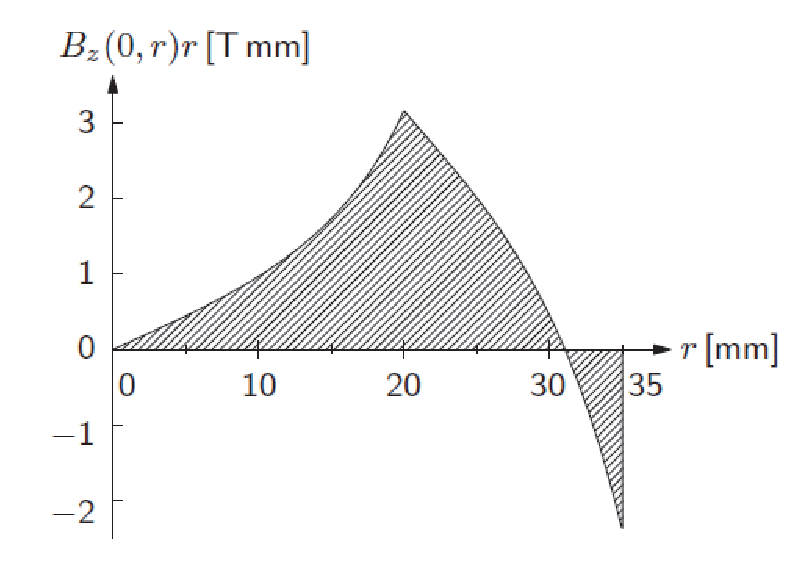
\includegraphics[scale=0.6]{chpt9/figs/fig9.8.eps}
	\caption{$B_z(0,r)r$ vs. $r$曲线。}
\end{figure}

\textbf{b) 钢板}\qquad 下面我们考虑钢板。
为了简化问题,我们首先假定钢板的磁导率无限大,即$\mu/\mu_o=\infty$。
接下来,为了模拟钢板对其上(即$z\ge -5$ mm)磁场的作用,
我们将钢板替换为一个和原线圈完全一样但至于板下的对称虚拟线圈,如图9.9所示。

通过证明虚拟线圈满足钢板在($r,z=-5\ \mathrm{mm}$)处的边界条件,
解释直接位于原线圈下的虚拟线圈能模拟理想钢板的效果。

\textbf{解:}$\mu/\mu_o=\infty$的理想钢板的边界条件是磁场切向分量(此处为轴向)在
板表面必须为零,即$B_z(z=-5\ \mathrm{mm})=0$。
也即,磁场必须以垂直钢板表面的形式穿入或传出。
与原线圈等同并且置于其下的线圈,根据对称性,可以满足上述边界条件。

\textbf{c) 钢板的场增强作用}\qquad 使用图9.9中的模型,计算线圈的中心场$B_z(0,0)$。
系统如图9.6,线圈载流为25 A。

\textbf{解:}由图9.7,没有钢板时,线圈通流25 A产生$[B_z(0,0)]_{w/o}\simeq 0.0863$ T。
有钢板时,我们必须加入中心点在$r=0$和$z=-10$ mm的虚拟线圈的贡献。
\begin{align*}%page570 第一个
[B_{z}(0,0)]_{with}&=[B_{z}(0,0)+B(z=10\ \mathrm{mm}mm,0)]_{w/o}\\
&\simeq 0.0863+0.711\simeq 0.1574\ \mathrm{T}
\end{align*}
等式右侧的第二项即虚拟线圈的贡献。
可见,钢板不足以令上方区域磁场翻倍---仅在$z=-5$ mm处恰好翻倍。
钢板似乎令$z=-5$ mm下方区域的磁场翻折到了其上方区域。
理想钢板的下方,磁场为零。

\begin{figure}
	\centering
	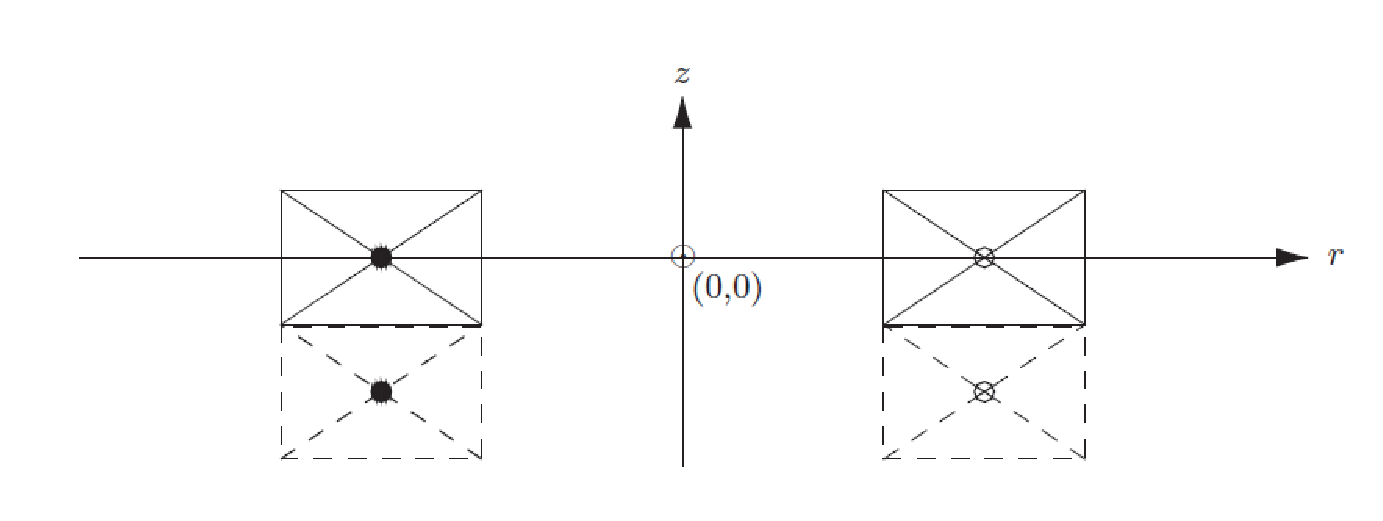
\includegraphics[scale=0.6]{chpt9/figs/fig9.9.eps}
	\caption{为建模钢板的效应而做的线圈安排。尺寸与图9.6相同。与原线圈等同的虚拟线圈置于
	原线圈下方,替代$\mu/\mu_o=\infty$的理想钢板。}
\end{figure}

\textbf{d) 钢板厚度}\qquad 为了确保我们对钢板的$\mu/mu_o\gg 1$假设有效,需保持钢板磁化强度$\mu_o M_{st}$小于1.25 T。计算所需钢板的最小厚度。

\textbf{解:}我们采用如下步骤:
1) 假定钢板为理想$\mu/\mu_o=\infty$;
2) 由图9.7,确定$z=-5$ mm处的径向位置$r=r_{\pm}$,在该处总$B_z$(实线圈和虚线圈)的方向改变---
在$0\le r\le r_{\pm}$区间$B_z$离开钢板,在$r\ge r_{\pm}$区间进入钢板;
3) 确定在$0\le r\le r_{\pm}$区间离开钢板的总磁通;
4) 令$\Phi_r(r=r_{\pm})$与在钢板$r=r_{\pm}$处径向总磁通相等。

理想钢板中总的轴向磁场是实线圈$B_z(-5\ \mathrm{mm},r)$的二倍---
因为虚线圈给出了等量的贡献。
注意到,$B_z(-5\ \mathrm{mm},r)=B_z(5\ \mathrm{mm},r)$。
$2 B_z(5\ \mathrm{mm},r)$和$2 B_z(5\ \mathrm{mm},r)r$的值在表9.5中给出。
$\int 2B_z rdr$由图9.10给出的$2B_z(5\ \mathrm{mm},r)r$线得到。
\begin{align*}%page571 第一个
\int_{0}^{r\pm}2B_{z}(z=5\ \mathrm{mm}mm,r)r\quad dr\simeq 7.22\times10^{-5}\ \mathrm{TM^{2}}\mbox{由图9.10}
\end{align*}
在$0\le r\le r_{\pm}$=31.56 mm区间穿出钢板的总磁通$Phi_{r_{\pm}}$于是为:
\begin{align*}%page571 第二个
\Phi_{r\pm}=2\pi(7.22\times 10^{-5}\ \mathrm{Tm^{2}})\simeq 45.4\times 10^{-5}\ \mathrm{Tm^{2}}
\end{align*}
这个磁通在$r=r_{\pm}$流入,等于通过钢板的总磁通$\Phi_{st}$:
\begin{align*}%page571 第三个
\Phi_{st}=\pi r_{\pm}\delta_{st}(\mu_{o}M_{st})=\Phi_{r\pm}
\end{align*}
解出$\delta_{st}$:
\begin{align*}%page571 第四个
\delta_{st}=\frac{\Phi_{r\pm}}{2r_{\pm}(\mu_{o}M_{st})}=\frac{45.4\times 10^{-5}\ \mathrm{Tm^{2}}}{2\pi(0.03156\ \mathrm{m})(1.25\ \mathrm{T})}\simeq 1.8\ \mathrm{mm}
\end{align*}
也即,$\sim$2 mm厚的钢板应当足够满足要求。
从表2.5,我们注意到as-cast钢在$\mu_o M$=1.25 T时有$(\mu/\mu_o)_{dif}=180$。

\begin{table}[htbp]\small
\centering
\caption{$2B_z(5\ \mathrm{mm},r)$和$2B_z(5\ \mathrm{mm},r)r$}  
\begin{tabular}{|c|c|c|}
\hline
\begin{tabular}[c]{@{}c@{}}r\\ $\left[\mathrm{mm}\right]$\end{tabular} & \begin{tabular}[c]{@{}c@{}}$2B_z(5\ \mathrm{mm},r)$\\ $\left[\mathrm{T}\right]$\end{tabular} & \begin{tabular}[c]{@{}c@{}}$2B_z(5\ \mathrm{mm},r)r$\\ $\left[\mathrm{T mm}\right]$\end{tabular} \\ \hline
\multirow{8}{*}{\begin{tabular}[c]{@{}c@{}}0\\ 5\\ 10\\ 15\\ 20\\ 25\\ 30\\ 31.56\end{tabular}} & \multirow{8}{*}{\begin{tabular}[c]{@{}c@{}}0.1640\\ 0.1675\\ 0.1788\\ 0.2010\\ 0.2377\\ 0.1282\\ 0.0344\\ 0\end{tabular}} & \multirow{8}{*}{\begin{tabular}[c]{@{}c@{}}0\\ 0.838\\ 1.788\\ 3.015\\ 4.754\\ 3.205\\ 1.032\\ 0\end{tabular}} \\
& & \\
& & \\
& & \\
& & \\
& & \\
& & \\
& & \\ \hline
\end{tabular}
\end{table}



\begin{figure}
	\centering
	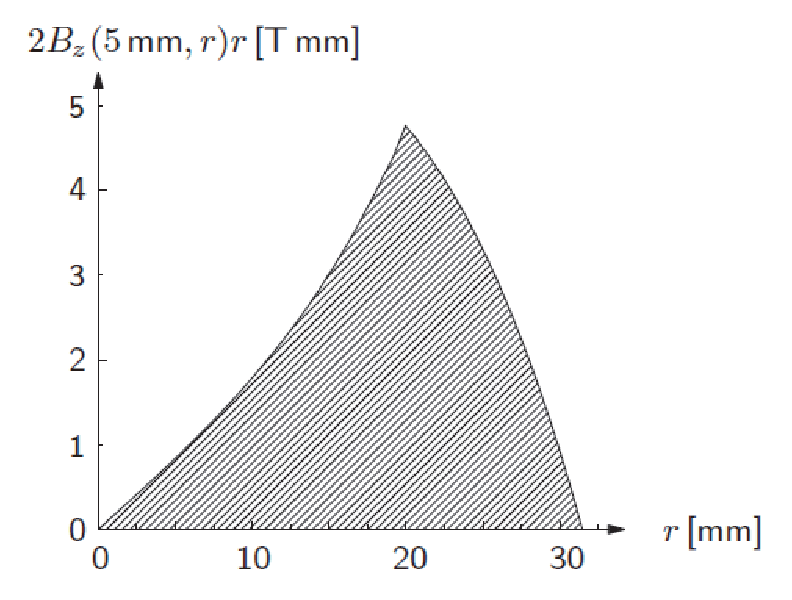
\includegraphics[scale=0.6]{chpt9/figs/fig9.10.eps}
	\caption{$B_z(5\ \mathrm{mm},r)r$ vs. $r$曲线。}
\end{figure}

那么钢板的外径$r_{od}$应当是多少呢?
理论上来说应该是无限大---当然不具操作性。
需要我们做的就是从$r_{pm}$到$r_{od}$积分$rB_z(r,5\ \mathrm{mm})$,
并令之满足如下条件:
\begin{align*}%page572 第一个
\int_{r\pm}^{r_{od}}B_{z}(r,z=5\ \mathrm{ mm})d\quad dr>\sim(0.8)\int_{0}^{r\pm}B_{z}(r,z=5\ \mathrm{ mm})r\quad dr
\end{align*}

也就是收,钢板应该能捕获至少内部区域($0\le r\le r_{\pm}$)穿出的磁通的80\%。
为了满足上述条件,$r_{od}$有约60 mm就够了。


\subsection{例C:平HTS扁平板的悬浮}
图9.11给出了一个厚为$\delta_d$、半径为$R_d$的HTS扁平板悬浮于两个嵌套线圈中心之上$z_\ell$的
系统截面图。嵌套线圈1和2的通流方向相反。
两个线圈均无骨架,置于钢板上。
HTS扁平板、线圈和钢板轴向对齐。
表9.6给出了两个线圈的参数。


\begin{table}[htbp]\small
\centering
\caption{线圈参数}  
\begin{tabular}{|l|c|c|}
\hline
参数 & 线圈1 & 线圈2 \\ \hline
绕组内径i.d.($2a_1$) $\left[\mathrm{mm}\right]$ & 40 & 20 \\ \hline
绕组外径o.d.($2a_2$) $\left[\mathrm{mm}\right]$ & 70 & 30 \\ \hline
绕组高度($2_b$) $\left[\mathrm{mm}\right]$ & 10 & 10 \\ \hline
Total turns($N_s$) & 150 & 50 \\ \hline
\end{tabular}
\end{table}

\begin{figure}
	\centering
	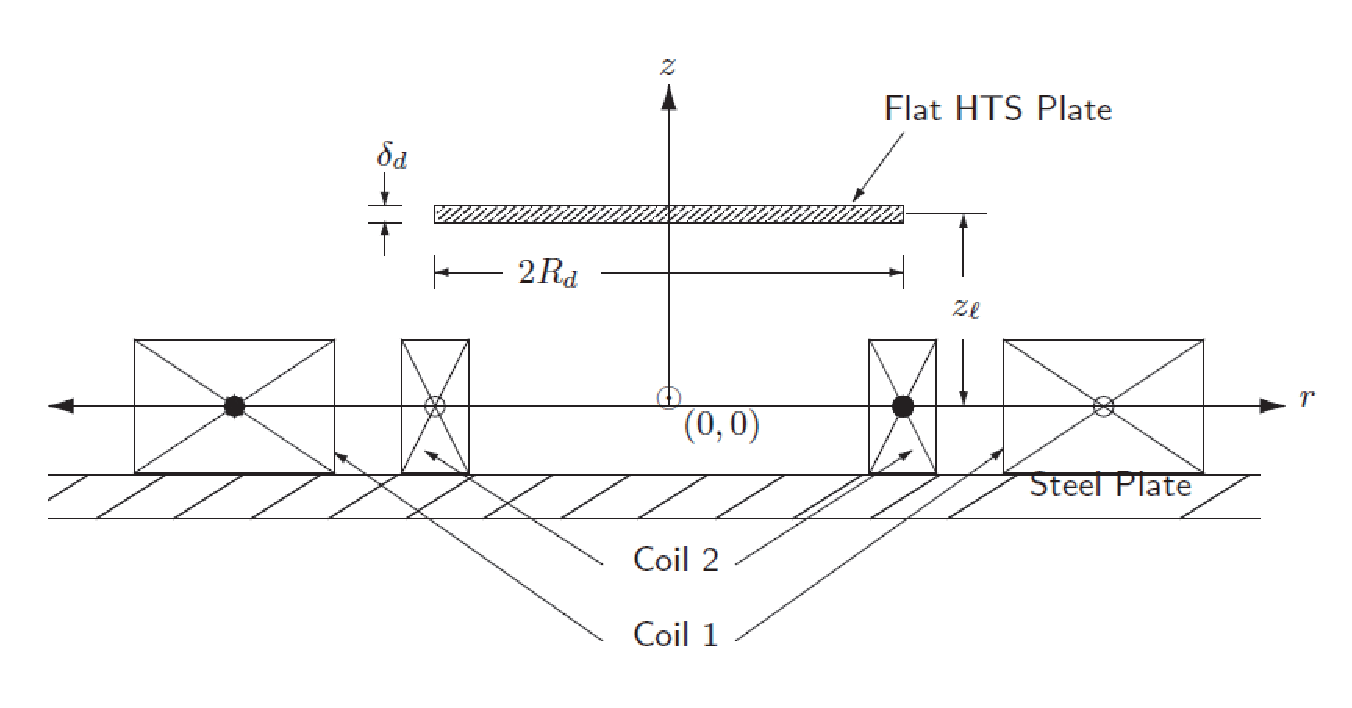
\includegraphics[scale=0.5]{chpt9/figs/fig9.11.eps}
	\caption{一个厚为$\delta_d$、半径为$R_d$的HTS扁平板悬浮于两个嵌套线圈中心之上$z_\ell$的
		系统截面图。嵌套线圈1和2的通流方向相反。
		两个线圈均无骨架,置于钢板上。该图在尺度上为近似值。}
\end{figure}

图9.12给出了在$z=0,5,7.5,10,12.5,15,17.5,20$ mm处的$B_z(z,r)$ vs. $r$曲线,
线圈1通流25 A,线圈2通流-15 A;
图9.13给出了在$r=5,10,12.5,15,17.5$ mm处的$B_z(z,r)$ vs. $z$曲线,线圈通流情况与9.12同。
这些图线都是不包括钢板的。

\begin{figure}
	\centering
	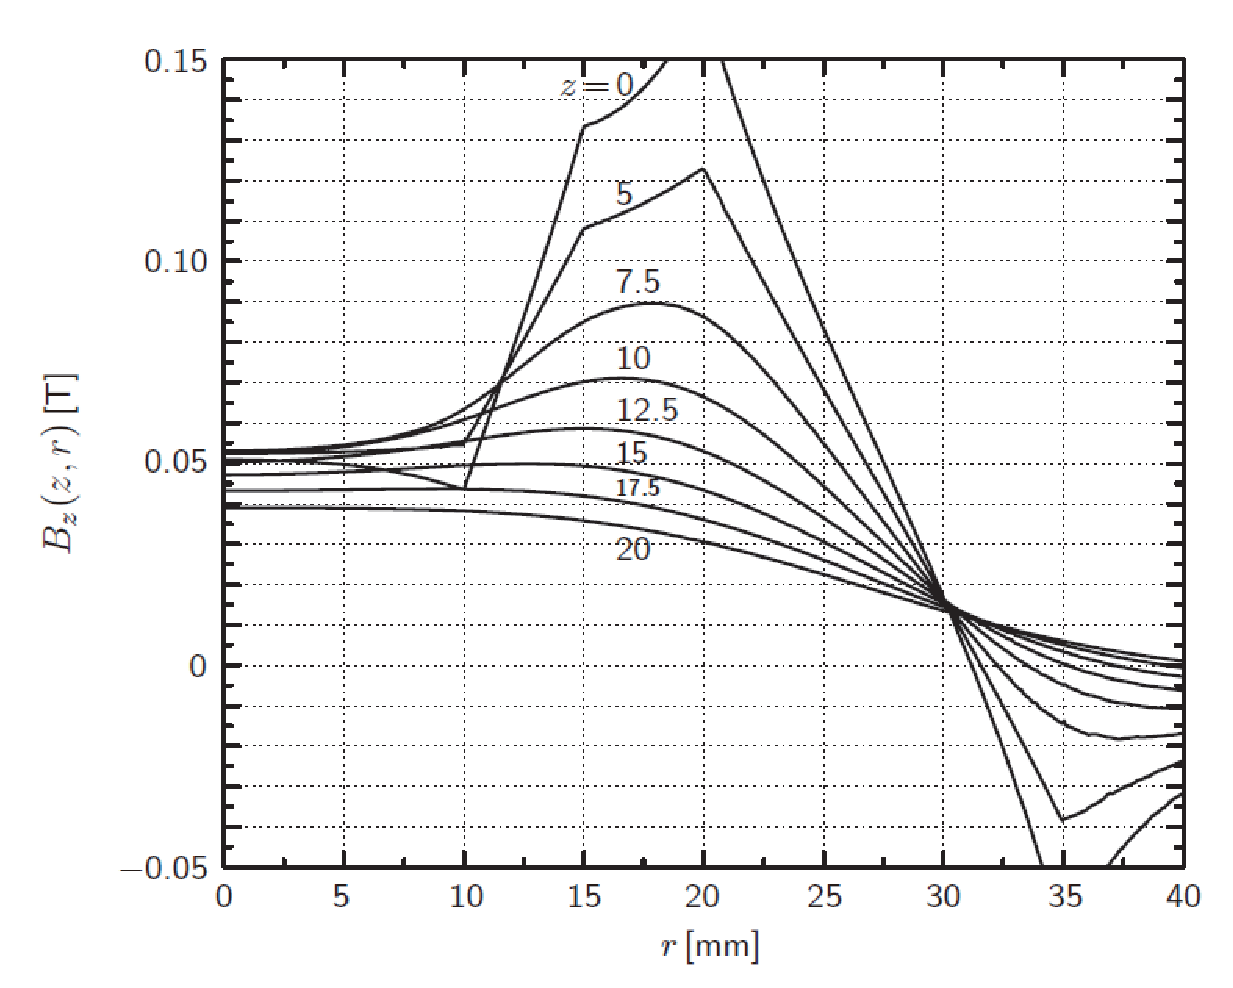
\includegraphics[scale=0.5]{chpt9/figs/fig9.12.eps}
	\caption{线圈1通流25 A,线圈2通流-15 A时,在$z=0,5,7.5,10,12.5,15,17.5,20$ mm处的$B_z(z,r)$ vs. $r$曲线。}
\end{figure}

\begin{figure}
	\centering
	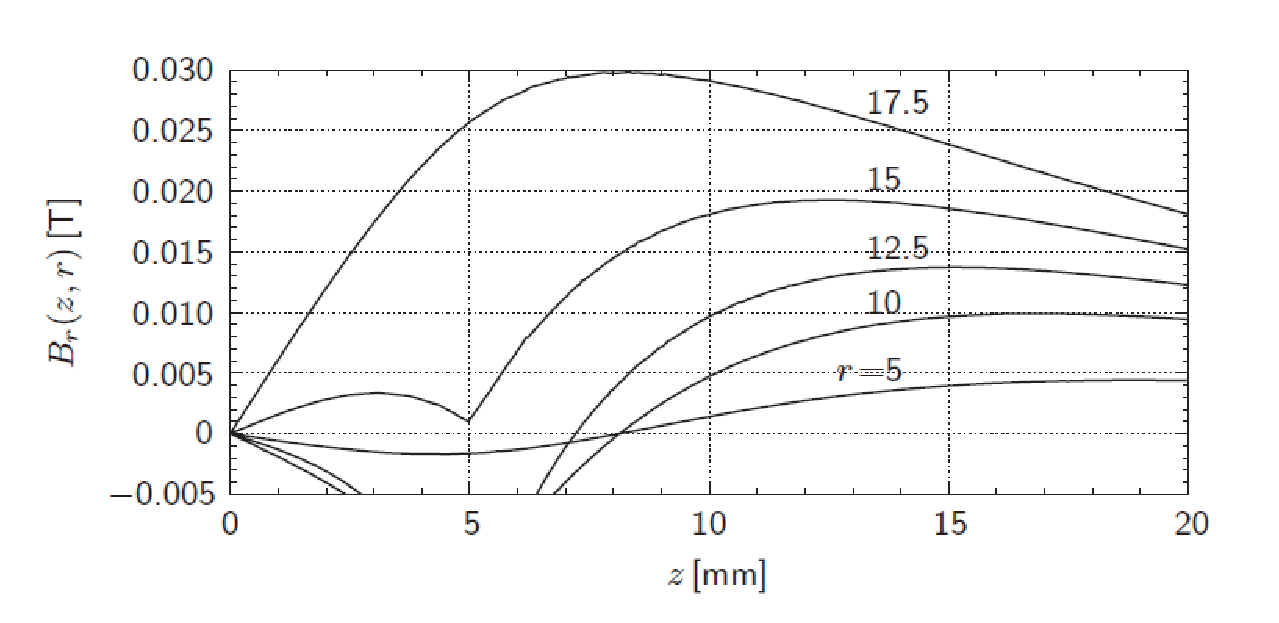
\includegraphics[scale=0.5]{chpt9/figs/fig9.13.eps}
	\caption{线圈1通流25 A,线圈2通流-15 A时,在$r=5,10,12.5,15,17.5$ mm处的$B_z(z,r)$ vs. $z$曲线。}
\end{figure}

\subsubsection{Q/A C:HTS扁平板的悬浮}
\textbf{a) 悬浮力---托举力}\qquad 假定HTS扁平板中感应出的超流电流$I_s$被约束在平板边缘内,
首先证明将平板悬浮于中心轴上方$z_\ell$的悬浮力$F_z(z_\ell)$可由下式给出:
\begin{align*}%page574 第一个
F_{z}(z_{\ell})=2\pi R_{d}I_{s}B_{r}(z_{\ell},R_{d})\tag{9.3a}
\end{align*}
式中,$B_{r}(z_{\ell},R_{d})$是在$(z_{\ell},R_{d})$处由两个线圈产生的径向场。

接下来,将平板建模为半径相同的无限长的圆柱,使其置于均匀轴向场中,轴向场
与Bean临界态场满足$H_z(z_\ell,R_d)\ll J_c R_d$。证明$F_z(z_\ell,R_d)$显式
依赖于$\delta_d$和$B_z(z_\ell,R_d)$。

\textbf{解:}在$H_z(z_\ell,R_d)\ll J_c R_d$条件下(其中,$J_c$是板材料的临界电流密度),
超流电流$I_s$被限制在厚度为$\delta_d$的表面薄层内。
假定该表面电流是均匀的,并止于其边缘。
我们可以令悬浮力$F_z(z_\ell,R_d)$与边缘处($r=R_d$)电流$I_s$上的洛伦兹力相等,其中后者定义为
$2\pi R_d,I_s$和$B_r(z_\ell,R_d)$之积。
\begin{align*}%page574 第二个
F_{z}(z_{\ell})=2\pi R_{d}I_{s}B_{r}(z_{\ell},R_{d})\tag{9.3a}
\end{align*}
根据Bean临界态模型,在$H_z(z_\ell,R_d)<H_p$(其中,$H_p=J_c R_d$为临界态场)时,
超流层厚度$\delta_{s}$为:
\begin{align*}%page574 第三个
\delta_{s}=\frac{H_{z}(z_{\ell},R_{d})}{J_{c}}=\frac{1}{J_{c}}[\frac{B_{z}(z_{\ell},R_{d})}{\mu_{o}}]\tag{a.1}
\end{align*}
也即,板内感应的总超流电流为:
\begin{align*}%page574 第四个
I_{s}=\delta_{d}\delta_{s}J_{c}=\delta_{d}[\frac{B_{z}(z_{\ell},R_{d})}{\mu_{o}}]\tag{a.2}
\end{align*}
联立方程9.3a和a.2,有:
\begin{align*}%page574 第五个
F_{z}(z_{\ell})=2\pi R_{d}\delta_{d}[\frac{B_{z}(z_{\ell},R_{d})B_{r}(z_{\ell},R_{d})}{\mu_{o}}]\tag{9.3b}
\end{align*}
方程9.3b表明,$F_z(z_\ell)\propto B_z(z_\ell,R_d)B_r(z_\ell,R_d)$。
也即,在这悬浮系统,两个线圈电流可以为不同的值来设定一个悬浮高度[9.5--9.9]。
同时注意到,只要满足$\delta_{s}\ll R_d$,即``大"$J_c$,$F_z(z_\ell)$就与$J_c$无关。

\textbf{b) YBCO板}\qquad 仍假定无钢板,使用图9.12和9.13中的$B_z(z,r)$和$B_r(z,r)$以及方程9.3b,
计算$R_d=15$ mm,$\delta_d=5$ mm的YBCO板,悬浮高度为$z_\ell=10$ mm时的悬浮力$F_z(z_\ell)$。
同时,计算该板的质量。证明在这个高度上,悬浮力可以撑起板的质量。YBCO的密度为$\rho=6.4\ \mathrm{g/cm^3}$。

\textbf{解:}由图9.12和9.13,我们有$B_z(z=10\ \mathrm{mm},r=15\ \mathrm{mm})\simeq 0.070$ T以及
$B_r(z=10\ \mathrm{mm},r=15\ \mathrm{mm})\simeq 0.0181$ T。于是:
\begin{align*}%page575 第一个
F_{z}(z_{\ell})&=2\pi R_{d}\delta_{d}[\frac{B_{z}(z_{\ell},R_{d})B_{r}(z_{\ell},R_{d})}{\mu_{o}}]\\ \tag{9.3b}
&\simeq\frac{2\pi(15\times 10^{-3}\ \mathrm{m})(5\times 10^{-3}\ \mathrm{m})(0.070\ \mathrm{T})(0.0181\ \mathrm{T})}{(4\pi\times 10^{-7}\ \mathrm{H/m})}\\
&\simeq 0.475\ \mathrm{N}(\simeq 48.5\ \mathrm{g})
\end{align*}

YBCO板的质量$m_p$为:
\begin{align*}%page575 第二个
m_{p}&=\pi R^{2}_{d}\delta_{d\varrho}\\
&=\pi(1.5\ \mathrm{cm})^{2}(0.5\ \mathrm{cm})(6.4\ \mathrm{g/cm^{3}})\simeq 23g
\end{align*}
可见,即使没有钢板,在$z_\ell$=10 mm处对板的悬浮力也两倍于板的质量。

\textbf{c) 感应超流}\qquad 继续假定无钢板,计算对同一个YBCO板,悬浮于$z_\ell$=10 mm处时的超流层厚度$\delta_s$。证明$\delta_s\ll R_d$。计算时取$J_c=10^8\ \mathrm{A/m}$。
同时计算$I_s$。

\textbf{解:}使用方程a.1,注意到$B_z(z_\ell,R_d)\simeq 0.070$ T,我们有:
\begin{align*}%page575 第三个
\delta_{s}=\frac{H_{z}(z_{\ell},R_{d})}{J_{c}}&=\frac{1}{J_{c}}[\frac{B_{z}(z_{\ell},R_{d})}{\mu_{o}}]\\\tag{a.2}
&\simeq\frac{(0.070\ \mathrm{T})}{(10^{8}\ \mathrm{A/m^{2}})(4\pi\times 10^{-7}\ \mathrm{H/m})}\simeq 0.56\ \mathrm{mm}
\end{align*}
所要求的条件$\delta_s\ll R_d$显然满足。
使用方程a.2的前两个方程,有:
\begin{align*}%page575 第四个
I_{s}&=\delta_{d}\delta_{s}J_{c}\qquad(a.2)\\\tag{a.2}
&\simeq(5\times 10^{-3}\ \mathrm{m})(0.56\times 10^{-3}\ \mathrm{m})(10^{8}\ \mathrm{A/m^{2}})\simeq 280A
\end{align*}
当板置于轴向场$B_z(R_d,z_\ell)$=0.07 T中,YBCO板内感应出超流电流280 A。

\textbf{d) 悬浮刚度}\qquad
推导$z=z_\ell$处悬浮刚度$k_z$的表达式。
计算$R_d$=15 mm; $\delta_s$=5 mm;$z_\ell$=10 mm条件下的$k_z$。

\textbf{解:}$z=z_\ell$处悬浮刚度为:
\begin{align*}%page576 第一个
k_{z}=-frac{\partial F_{z}(z,R_{d})}{\partial_{z}}|_{z_{\ell}}\tag{d.1}
\end{align*}
负号表示$F_{z}(z,R_{d})$随$z$减小而增大。
联立方程9.3b和d.1,我们有:
\begin{align*}%page576 第二个
k_{z}=-2\pi R_{d}\delta_{d}\{[\frac{B_{r}(z_{\ell},R_{d})}{\mu_{o}}]\frac{\partial B_{z}(z,R_{d})}{\partial_{z}}|_{\ell}+[\frac{B_{z}(z_{\ell},R_{d})}{\mu_{o}}]\frac{\partial B_{r}(z,R_{d})}{\partial z}|_{\ell}\}\tag{9.4}
\end{align*}
向方程9.4中代入合适的参数值,有:
\begin{align*}%page576 第三个
k_{z}\simeq&-2\pi(15\times 10^{-3}\ \mathrm{m})(5\times 10^{-3}\ \mathrm{m})\\
&\times[(\frac{0.181\ \mathrm{T}}{4\pi\times 10^{-7}\ \mathrm{H/m}})(-5.2\ \mathrm{T/m})+(\frac{0.070\ \mathrm{T}}{4\pi\times 10^{-7}\ \mathrm{H/m}})(1.1\ \mathrm{T/m})]\\
=&-2\pi(75\times 10^{-6}\ \mathrm{m^{2}})(\frac{10^{7}}{4\pi}\ \mathrm{m/H})(-0.0943\ \mathrm{T^{2}/M}+0.758\ \mathrm{T^{2}/m})\\
\simeq &6.9\ \mathrm{N/m}
\end{align*}
由图9.12知,在$R_d=15$ mm和$z_\ell=$10 mm时,$k_z>0$;
于是我们得到,在小的轴向位移下,板的悬浮是稳定的,也即,
如果将板往下推,悬浮力会增加。

\textbf{e) 共振频率}\qquad 计算悬浮于$z_\ell$=10 mm时,该YBCO板轴向运动的共振频率$\nu_z$。
使用b)中计算得到的YBCO板质量$m_p$=23 g。

\textbf{解:}对一个简单的质量($m$)--弹簧($k$)系统,共振频率$\nu$为:
\begin{align*}%page576 第四个
\nu=\frac{1}{2\pi}\sqrt{\frac{k}{m}}
\end{align*}
于是,
\begin{align*}%page576 第五个
\nu_{z}&\simeq\frac{1}{2\pi}\sqrt{\frac{(6.9\ \mathrm{N/m})}{(23\times 10^{-3}\ \mathrm{kg})}}\\
&\simeq 3\ \mathrm{Hz}
\end{align*}
当板垂直位移时,在频率为3 Hz时会发生振荡。

\begin{figure}
	\centering
	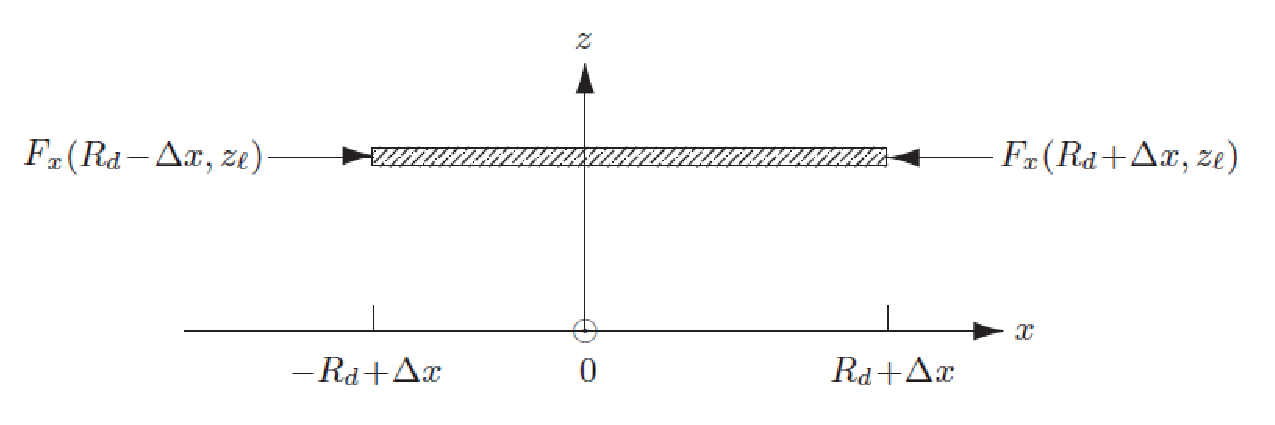
\includegraphics[scale=0.6]{chpt9/figs/fig9.14.eps}
	\caption{悬浮的HTS板在水平向($+x$)移动$\Delta x$时的截面图。$y$方向为纸面向内。}
\end{figure}

\textbf{f1) 水平稳定性1}\qquad
证明HTS板在悬浮于$z_\ell$=10 mm时,对小水平位移($r$轴或这里的$x$轴)是稳定的。
假设板内感应超流电流限制在边缘的一个薄层$\delta_s$内。
同时,不计钢板。

\textbf{解:}在水平($x$轴)方向,$F_x$正比于$I_s$和$B_z$的叉积。
考虑如图9.11所示的与线圈轴向对齐悬浮的HTS板。
$F_x(z_\ell,R_d)$是$-x$方向的,因为$I_s(z_\ell,R_d)$是$-y$方向的、$B_z(x=0)$是$+z$方向的:
$F_x(z_\ell,R_d)\propto -I_s(z_\ell,R_d)B_z(z_\ell,R_d)\vec{i_x}$。
另一方面,$F_x(z_\ell,-R_d)$是$+x$方向的,因为$I_s(z_\ell,R_d)$是$+y$方向的、$B_z(x=0)$仍是$+z$方向的:
$F_x(z_\ell,-R_d)\propto +I_s(z_\ell,R_d)B_z(z_\ell,R_d)\vec{i_x}$。
因为$B_z(z_\ell,R_d)=B_z(z_\ell,-R_d)$,$I_s(z_\ell,R_d)=-I_s(z_\ell,-R_d)$,我们有:
\begin{align*}%page577 第一个
F_{x}(z_{\ell},R_{d})+F_{x}(z_{\ell},-R_{d})&\propto-I_{s}(z_{\ell},R_{d})+I_{s}(z_{\ell},R_{d})B_{z}(z_{\ell},-R_{d})\\
&=0
\end{align*}
也即,在$x=0$处板中心的净水平力为零。

现在考虑板在$+x$向的微小位移$\Delta x$,如图9.14所示。这时,我们有:
\begin{align*}%page577 第二个
F_{x}(z_{\ell},R_{d}+\Delta x)+F_{x}(z_{\ell},-R_{d}+\Delta x)\propto-&I_{s}(R_{d}+\Delta x)B_{z}(z_{\ell},R_{d}+\Delta x)\\
&+I_{s}(-R_{d}+\Delta x)B_{z}(z_{\ell},-R_{d}+\Delta x)\tag{f1.1}
\end{align*}
我们可以假设$I_{s}(z_{\ell},R_{d}+\Delta x)\simeq I_{s}(z_{\ell},R_{d})$,
$I_{s}(z_{\ell},-R_{d}+\Delta x)\simeq I_{s}(z_{\ell},-R_{d})$。
同时,因为$I_{s}(z_{\ell},R_{d})=-I_{s}(z_{\ell},-R_{d})$,方程f1.1可以化简为:
\begin{align*}%page577 第三个
F_{x}(z_{\ell},R_{d}+\Delta x)+F_{x}(z_{\ell},-R_{d}+\Delta x)\propto-I_{s}(R_{d})&[B_{z}(z_{\ell},R_{d}+\Delta x)\\
&-B_{z}(z_{\ell},-R_{d}+\Delta x)]\tag{f1.2}
\end{align*}

由图9.12,我们注意到在$z=10$ mm($z_\ell$)和$R_d$=15 mm附近,
在``小"$\Delta$下有$B_z(z_\ell,R_d+\Delta x)>B_z(z_\ell,-R_d+\Delta x)$。
于是,在小的水平为以下,水平力可令之恢复。
注意到图9.12中,$z=10$ mm的迹线峰值出现在$r=16.5$ mm;
$\partial B_z/\partial r$随后改变符号,当$\Delta x> 4$ mm后,板不再稳定。
图9.12中对应$z\ge 12.5$ mm的迹线表明,板在$z_\ell\simeq 12.5$ mm时临界稳定,
在$z_\ell> 12.5$ mm后不稳定。

\textbf{f2) 水平稳定性2}\qquad
通过展示水平弹性常数$k_x$在$r=R_d$时为正,即$k_x\equiv -\partial F_x"z_\ell,r)/\partial x>0$,
证明板对小的径向位移是稳定的。
同时确定在$z=10$ mm和$x=$15 mm时,$k_x$和水平方向自然频率$\nu_x$的数值。

\textbf{解:}为了量化f1)中的分析,考虑作用于最右侧电流长度微元$\Delta y$上的力微元$\Delta f_{x+}$:
$\Delta f_{x+}=I_s\Delta y B_z(R_d+\Delta x)$。
$\Delta f_{x+}$仅由对应最左侧元素上的力$\Delta f_{x-}$部分平衡:
$\Delta f_{x-}=I_s\Delta y B_z(R_d-\Delta x)$。
净力微元$\Delta f_{x}=\Delta f_{x+}+\Delta f_{x-}$为:
\begin{align*}% page578 f2.2
\Delta f_x(z,R_d)=2I_s\Delta y\frac{\partial B_z(z,r)}{\partial r}\mid_{R_d}\Delta x \tag{f2.2}
\end{align*}
单位电流长度的净力为$\Delta f_{x}/\Delta y$。
如果该力在周向是恒定的,合力$\Delta F_x$将为$2R_d\times \Delta f_x$。
实际上,$\Delta f_{x}/\Delta y$在周向随$\sqrt{1-(r/R)^2}$变化;
平均值是峰值的$\pi/4$:
\begin{align*}% page578 第二个f2.2
\Delta F_x(z,R_d)=\pi R_dI_s\frac{\partial B_z(z,r)}{\partial r}\mid_{R_d}\Delta x \tag{f2.2}
\end{align*}
于是,$k_x$由下式给出:
\begin{align*}% page578第三个
k_x(z,R_d)=\frac{\Delta F_x(z,R_d)}{\Delta x}=\pi R_dI_s\frac{\partial B_z(z,r)}{\partial r}\mid_{R_d}
\end{align*}
在以下条件下计算$k_x$:$R_d$=15 mm;$I_s$=280 A;$\partial B_z(z_\ell,r)/\partial r$=1.08 T/m(在$z_\ell=10$ mm和$R_d=15$ mm时)。
\begin{align*}% page578 第四个
k_x(z_\ell,R_d)=2(15\times 10^{-3}\ \mathrm{m})(280\ \mathrm{A})(1.08\ \mathrm{T/m})\simeq 14.2\ \mathrm{N/m}
\end{align*}
与$k_z(z_\ell,R_d)$相比,水平刚度$k_x(z_\ell,R_d)$差不多翻倍。

水平方向的自然频率$\nu_x$为:
\begin{align*}% page578 f2.4
\upsilon_x=&\frac{1}{2\pi}\sqrt{\frac{k_x}{m_p}}  \\\tag{f2.4}
\simeq&\frac{1}{2\pi}\sqrt{\frac{14.2\ \mathrm{N/m}}{(23\times 10^{-3}\ \mathrm{kg})}}\simeq 4\ \mathrm{Hz}
\end{align*}
这些数值和实测值在同一量级[9.5,9.6]。

\textbf{g) 功率需求}\qquad 如果忽略液化氮的功率可以忽略,
将铜线圈浸泡于一个大气压下的液氮池中是节能的。
计算通流为25 A的线圈1和通流为15 A的线圈2,运行于77.3 K液氮中所需的总电功率$P_T=P_1+P_2$。
假定各线圈的空间因数$\lambda$均为0.785。
导体铜在77 K时的电阻率取为$\rho_{cd}$=2.5 n$\Omega$。

\textbf{解:}由方程3.112,我们有:
\begin{align*}% page579 3.112
P&=\rho_{cd}J^2\lambda a_{1}^{3}2\pi\beta(\alpha^2-1) \\\tag{3.112}
&=\rho_{cd}\frac{(\lambda J)^2}{\lambda}a_{1}^{3}2\pi\beta(\alpha^2-1)
\end{align*}
代入$\lambda J=NI/2b(a_2-a_1)=NI/2a_1^2\beta(\alpha-1)$,$P$成为:
\begin{align*}% page579 g.1
P=\frac{\pi\rho_{cd}(NI)^2(\alpha+1)}{2\lambda a_1\beta(\alpha-1)} \tag{g.1}
\end{align*}

对线圈1有$a_1=20\times 10^{-3}$ m; $\alpha=2a_2/2a_1$=70 mm/40 mm=1.75;
$\beta=2b/2a_1=$10 mm/40 mm=0.25。方程g.1给出:
\begin{align*}% page579 第三个
P_1=\frac{\pi(2.5\times 10^{-9}\ \mathrm{\Omega m})(150\times 25\ \mathrm{A})^2(1.75+1)}{2(0.785)(20\times 10^{-3}\ \mathrm{m})(0.25)(1.75-1)}\simeq 52\ \mathrm{W}
\end{align*}
类似的,线圈2:
\begin{align*}% page579第四个
P_2=\frac{\pi(2.5\times 10^{-9}\ \mathrm{\Omega m})(50\times 15\ \mathrm{A})^2(1.5+1)}{2(0.785)(10\times 10^{-3}\ \mathrm{m})(0.5)(1.5-1)}\simeq 3\ \mathrm{W}
\end{align*}
于是,两线圈的总功耗为约55 W。

\textbf{h) 液氮挥发率}\qquad 在功耗为55 W条件下,计算液氮的近似挥发率$\dot{Q}_\ell$。

\textbf{解:}一定功率下的液氮挥发率为:
\begin{align*}% page579 h.1
\dot{Q}_\ell=\frac{P}{h_L} \tag{h.1}
\end{align*}
式中,$h_L$为液氮的汽化潜热。由表4.2知$h_L=161\ \mathrm{J/cm^3}$,方程h.1成为:
\begin{align*}% page579 最后一个
\dot{Q}_\ell&=\frac{(55\ \mathrm{W})}{(161\ \mathrm{J/cm^3})}=0.34\ \mathrm{cm^3/s}=1224\ \mathrm{cm^3/h} \\
&\sim 1\ \mathrm{liter/h}
\end{align*}
本系统长期运行时,安装线圈的低温容器需要以约1 L/h的速率补充液氮。

\begin{figure}
	\centering
	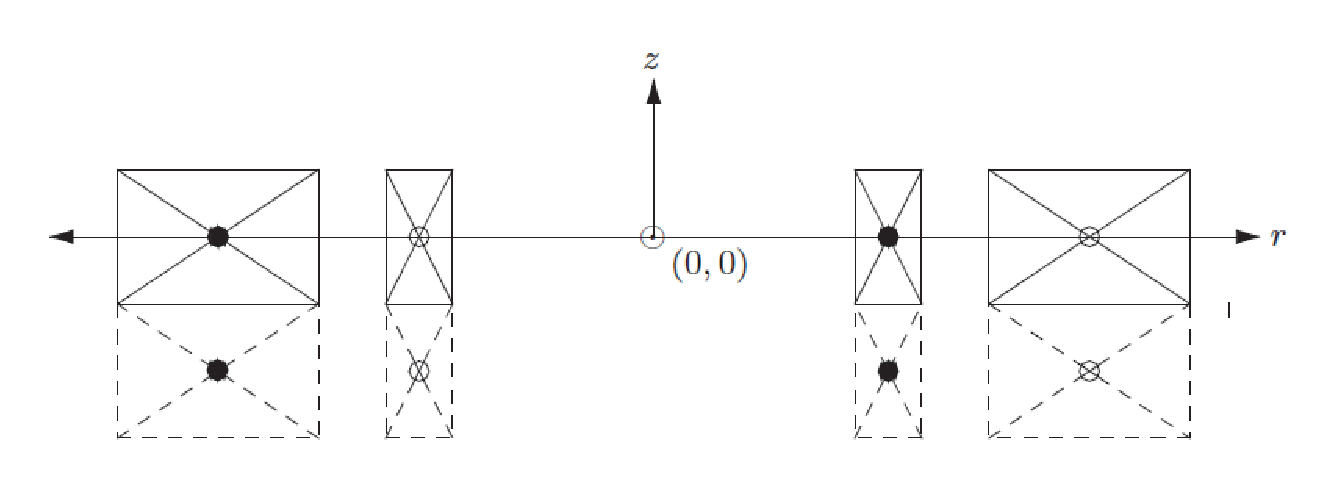
\includegraphics[scale=0.6]{chpt9/figs/fig9.15.eps}
	\caption{将图9.11建模为存在钢板时的线圈排列。}
\end{figure}

我们现在开始研究图9.11中的钢板的影响。
为了简化问题,我们首先假设钢板为无限磁导率的,即$\mu/\mu_o=\infty$。
接下来,为了计入钢板对板上部(即$z\ge-5$ mm)的磁场的影响,
我们将钢板替换为与原始线圈组一致的虚线圈组,安装方法如图9.15所示。
注意到,各线圈均假定为不含骨架。

\textbf{i) 有钢板}\qquad 现在我们计算存在理想钢板时对$z_\ell=10$ mm处悬浮板的力。
同时,讨论轴向和径向的稳定性。

\textbf{解:}无钢板时,由图9.12和9.13我们有$[B_z(z_\ell,R_d)]_{w/o}\simeq 0.070$ T和
$[B_r(z_\ell,R_d)]_{w/o}\simeq 0.019$ T。
有理想钢板时,位于$z=-10$ mm的虚线圈的贡献也必须计入。
\begin{align*}% page580 第一个
[B_z(z_\ell,R_d)]_{\mathrm{with}}&=[B_z(z_\ell,R_d)+B_z(z\ell+10.0\ \mathrm{mm},R_d)]_{\mathrm{w/o}} \\
&\simeq(0.070\ \mathrm{T})+(0.036\ \mathrm{T})=0.106\ \mathrm{T}\\
[B_r(z_\ell,R_d)]_{\mathrm{with}}&=[B_r(z_\ell,R_d)+B_r(z\ell+10.0\ \mathrm{mm},R_d)]_{\mathrm{w/o}} \\
&\simeq(0.018\ \mathrm{T})+(0.015\ \mathrm{T})=0.033\ \mathrm{T}
\end{align*}
向方程9.3b中代入上述磁场值,我们得到:
\begin{align*}% page580 9.3b
F_z(z_\ell,R_d)=&2\pi R_d\delta_d\left[\frac{B_z(z_\ell,R_d)B_r(z_\ell,R_d)}{\mu_o}\right]  \\\tag{9.3b}
\simeq&\frac{2\pi(15\times 10^{-3}\ \mathrm{m})(5\times 10^{-3}\ \mathrm{m})(0.106\ \mathrm{T})(0.033\ \mathrm{T})}{(4\pi\times 10^{-7}\ \mathrm{H/m})} \\
\simeq& 1.31\ \mathrm{N}(\simeq 134\ \mathrm{g})
\end{align*}

于是,存在理想钢板时,系统产生了一个六倍于板重量的悬浮力,也即,
板能够撑起大于110 g的负载。
该系统在轴向是稳定的($k_z\simeq$6.9 N/m),在水平向也是稳定的($k_x\simeq$9.1 N/m)。


\section{例D:HTS``环"磁体}
有一种只有HTS可能而LTS不可能的磁体设计,它由许多HTS块或环形版堆叠而成。
图9.16给出了示意截面图,各单元内径$2a_1$而外径$2a_2$。分别是:
a) 块材环片,厚度为$\delta_b$;b) 薄板环片,总厚度$\delta_p$,超导薄膜厚度$\delta_f$;
c) ``环"磁体,总高度为$2b$,由一些块材环片或薄板环片堆叠而成。
注意到环磁体既无分段,也无终端。

对YBCO和其他稀土类HTS块材[9.10-9.14],$2a_1,2a_2$的实际可得值分别为40-60 mm
和70-100 mm,这使得采用这种块材环片来开发小型NMR磁体具有了现实可行性[9.15]。
同时,因为宽为40-100 mm的涂层YBCO导体已开发出来[9.16,9.17],
在不久的将来,在一根宽的涂层导体用模具压出环片是可能的。

典型的,块材环片厚度$\delta_b\sim 10$ mm,
板环片厚度$\delta_p\sim 100\ \mathrm{\mu m}$,$\delta_f\sim 1\ \mathrm{\mu m}$。
这样,一个$2b$=300 mm的环形磁体将包括30个块材环片或约3000个板环片。
因为各环片都是回环,环磁体的励磁过程和线绕磁体存在很大的不同---参见问题1.2。

\begin{figure}
	\centering
	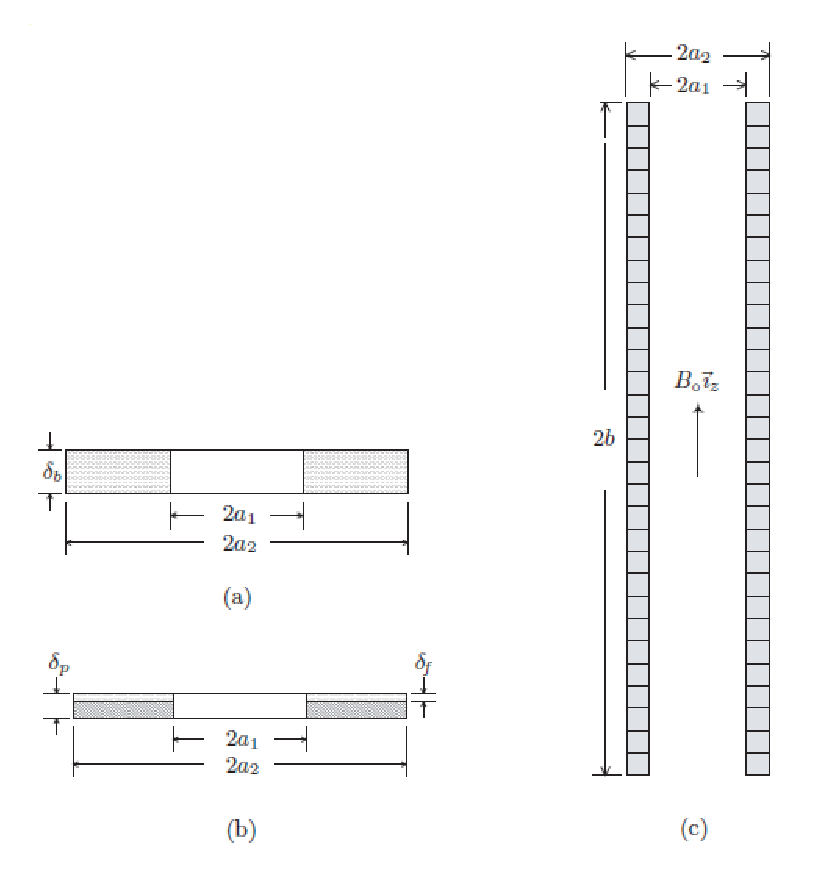
\includegraphics[scale=0.7]{chpt9/figs/fig9.16.eps}
	\caption{示意截面图,各单元内径$2a_1$而外径$2a_2$。分别是:
		a) 块材环片,厚度为$\delta_b$;b) 薄板环片,总厚度$\delta_p$,超导薄膜厚度$\delta_f$;
		c) ``环"磁体,总高度为$2b$,由一些块材环片或薄板环片堆叠而成。}
\end{figure}

\subsubsection{Q/A D:HTS``环"磁体}
\textbf{a) 总(工程)电流密度}\qquad 假定环磁体是``长"的,即$\beta\gg 1$,计算
在$2a_1$=50 mm, $2a_2$=75 mm, $2b$=300 mm时,
产生轴向中心场$B_o=11.74$ T(对应500 MHz的NMR)所需的总电流密度$\lambda J$或$J_e$。

\textbf{解:}由于$\alpha=1.5,\beta=6$,这个``螺管"磁体可以视为``长"的,
即磁体中心场$B_o=B_z(0,0)$可由方程3.111e给出:
\begin{align*}% page582 3.111e
B_z(0,0)=\mu_o\lambda Ja_1(\alpha-1) \tag{3.111e}
\end{align*}
注意到$B_z(0,0)$与磁体长度无关,正比于``绕组"构造。
从方程3.111e中解出$\lambda J$,我们得到:
\begin{align*}% page582 第二个
\lambda J=\frac{B_z(0,0)}{\mu_oa_1(\alpha-1)}=\frac{(11.74\ \mathrm{T})}{(4\pi\times 10^{-7}\ \mathrm{H/m})(0.025\ \mathrm{m})(1.5-1)}=7.5\times 10^8\ \mathrm{A/m^2}
\end{align*}

\textbf{b) 电流密度要求---块材片 vs. 板片}\qquad
讨论块材片和板片的总(工程)电流密度。

\textbf{解:} 尽管图9.16c给出了的绕组空间完全由块材片或板填满,
但实际的环磁体中,相邻片间还有一个``薄"的垫片。
这些垫片不仅加强了绕组对磁场力的强度,还以沿轴向不同位置采用不同厚度垫子
的形式用来调节轴向场分布。

\textbf{块材片}\qquad 因为垫片占据不超过总绕组空间的$\sim 10\%$,
$\lambda J\simeq J_c$,其中$J_c$是块材临界电流密度。
也即,在块材片磁体中,材料临界电流密度应当不是限制产生11.74 T或更大中心场的因素。

\textbf{板片}\qquad 以涂层YBCO导体为例,它还复合有其他非超导材料(如缓冲层、基底,其厚度
表示为$\delta_p-\delta_f$)。$\delta_p$和$\delta_f$的典型值分别是
75-100 $\mu$m和1 $\mu$m。于是,为了实现总电流密度$10^8--10^9\ \mathrm{ A/m^2}$,
YBCO膜的$J_c$必须至少达到$10^{10}\ \mathrm{ A/m^2}$,
该值仅在温度低于77 K时才能达到。

\textbf{c) 励磁技术}\qquad 讨论励磁一个``大型"和``高场"的环磁体的方法。

\textbf{解:}通常来讲,改变超导回路的磁通是不可能的,除非部分回路处于正常态---
``磁通门"必须要打开。
于是,甚至不可能励磁一个超导环(问题1.2),更遑论一个完全闭合的、保持超导态超导磁体。

如讨论7.4所研究的,励磁``常规"持续运行模式的磁体的一个方法是使用持续电流开关(PCS)。

另一个经常使用的技术是将未励磁且已处于超导态的线绕超导磁体(或块材片)置于一个脉冲场磁体的
室温孔中。
升降脉冲磁场的快速变化加热部分或大部分超导磁体,从而允许磁通进入。
确保超导磁体充分冷却后,可让磁体回到完全超导态,捕获部分脉冲磁场,成为持续模式的磁场。
本技术的缺点是:1) 难于精确控制最终持续模式磁场的水平,因为它苛刻的依赖于加热/冷却条件;
2) 对一个大型高场磁体,该脉冲磁体自身将变得很大,且需精心制作。

为了励磁大型高场环磁体,DC超导外场是一个最好的选项。
图9.17给出了本技术励磁环磁体的一个步骤的以试图,这里给出的是无垫片的环片堆叠磁体,
中心部分为槽型(参见问题3.7)。
励磁环磁体的步骤分为以下5步:
\begin{figure}
	\centering
	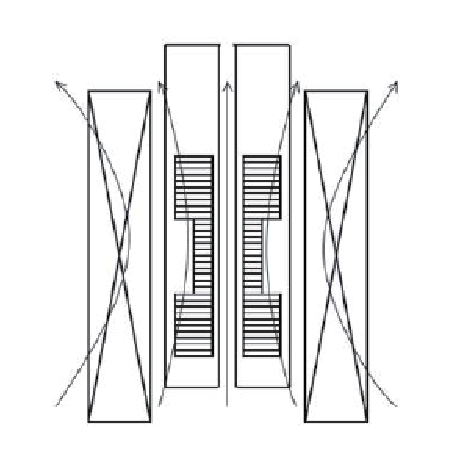
\includegraphics[scale=0.8]{chpt9/figs/fig9.17.eps}
	\caption{环磁体在使用某励磁环磁体技术第2步之后的示意图。
	磁体/低温容器单元,仍处于室温,置于外部DC超导磁体的室温孔内,暴露于外磁体的磁场中。}
\end{figure}

\begin{figure}
	\centering
	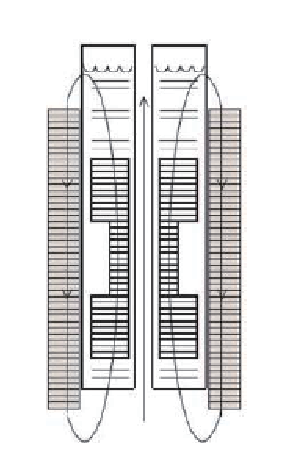
\includegraphics[scale=0.8]{chpt9/figs/fig9.18.eps}
	\caption{环磁体在励磁第5步之后的示意图。}
\end{figure}

\begin{enumerate}
	\item 将室温的磁体/低温容器单元置于外部DC超导磁体室温孔中。
	\item 在环磁体处于正常态时,将之暴露于外部磁体产生的磁场中(图9.17)。图中示意的画出了磁力线。
	\item 将环磁体冷却至完全超导态。因为环片是第II类超导体,磁场线在环磁体冷却至转变温度过程中基本维持不变。
	\item 缓慢将外部磁体放电至零,在各环片中建立起超流分布,反过来它将产生持续模式的磁场。这个过程
	叫做``磁场冷却"。
	\item 将外部磁体中移出磁体/低温容器单元,在其外侧安装由钢片组成的场屏蔽设备。步骤5之后的总体装配示意图如图9.18所示。	
\end{enumerate}

\textbf{d) 场屏蔽}\qquad 我们希望尽量减小磁体外部的边缘场。
如图9.18所示,环磁体可以由钢环片构成场屏蔽。
使用以下参数估算钢环片的外径$D_{so}$:
$D_{si}$ = 225 mm; $2a_1$ = 50 mm;
$2a_2$=75 mm; $B_z(0, 0)\equiv B_o$=11.74 T; $\mu_o M_s$=1.25 T。

\textbf{解:}因为基本上全部室温孔的轴向磁通都通过内径$D_{si}$、外径$D_{so}$的钢片屏蔽体,根据磁通守恒有:
\begin{align*}% page584 d.1
\frac{\pi}{3}(a_{2}^{2}+a_2a_1+a_{1}^{2})B_o\simeq\frac{\pi}{4}(D_{so}^{2}-D_{si}^{2})\mu_oM_s \tag{d.1}
\end{align*}
式中,$B_o$是中心场。
方程d.1的等式左侧表示磁体室温孔内($\pi B_o a_1^2$)加上$a_1$到$a_2$区间的环形域上的总磁通。
其中$B(r)=B_o(a_2-r)/(a_2-a_1)$,从$a_1$时的$B_o$线性降至$a_2$时的0;$M_s$是钢的磁化强度,
足够低以使其在$\mu\ge100\mu_o$时有效。
将参数值代入方程d.1,我们得到$D_{so}\simeq 296$ mm。

注意到,对于这个$D_{so}\simeq$296 mm的磁体系统,钢环片屏蔽体在径向占据大量空间。
不过,产生11.74 T中心场的径向尺度仅为$\sim 0.15$m的屏蔽磁体应视为相当紧凑了。

\textbf{e) 垫片}\qquad 相连HTS环片之间的垫片可以满足环磁体的若干关键要求。
给出哪些要求得到了满足,并提出合适的垫片材料。

\textbf{解:}这些要求包括:1) 机械加强;2) 热稳定性;3) NMR磁体的场均匀性。

\textbf{机械性能}\qquad 以11.7 T为例,在50 mm内径75 mm外径环片中洛伦兹力诱导的最大应力
$\sim 270$ MPa,这要高于YBCO块材的强度。
HTS环片之间插入的高强度垫片可以抗住这个负荷的大部分。
垫片的一个合适的选项是高强度的Cu-Ag合金片[9.18],
它最初用于高场Bitter磁体。
该材料的极限强度接近1000 MPa,杨氏模量$\sim 150$ GPa,
和铜的热导率几乎相同。

\textbf{热性能}\qquad 在场冷却阶段外部电磁体放电时,交流损耗,主要是磁滞损耗,将加热块材[9.19,9.20]。
这里,磁场放电速率可减小以限制温升。
使用强而热导率好的垫片仍是我们需要的:
上文给出的适合机械性能的Cu/Ag合金片同样也满足热性能。

\textbf{场均匀性}\qquad 通过控制特定轴向位置的垫片的厚度可以实现磁体中心特定的空间场均匀性。
这里,仅厚度是重要的。

\textbf{f) 块材 vs. 板}\qquad 比较块材环片和板环片,给出两个选项的优势和劣势,包括制造难易程度。

\textbf{解:} 两个选项各有优劣,简要描述如下:

\textbf{块材}\qquad 如b)中已指出,块材环片磁体的总电流密度接近材料的临界电流密度$J_c$:
这是块材的最大优势。
于是,当下可用的HTS块材片可用于组装建造可以产生12 T及以上磁场的环磁体。
最大的劣势可能是它的厚度:10 mm。
各环片中产生的感应电流和可能不均匀,令其难于实现既定的场分布。
另一个弱点是块材环片的制造,因为每一个盘的中心部分必须被切掉。
这个钻孔过程可能非常耗时,并可能损坏环片的超导性能。

\textbf{板}\qquad 块材的优势使板的劣势,反之亦然。
于是,使用环片建造一个高场的环磁体,超导体的$J_c$必须进一步提高,
或超导薄膜的厚度必须进一步增加,或非超导材料的组分必须减少。
最大的优势使超导膜的厚度($\sim$1 $\mu$m)。
相比于块材环片磁体,它更易于调节场的空间均匀性。
最后,相比于块材片,它可以更容易、进而更便宜的大规模生产:
简单地使用模具从宽的(例如100 mm)涂层超导体带上``冲"出来。


\textbf{g) 稳定性}\qquad 简要讨论环磁体的热稳定性。

\textbf{解:}环磁体的运行温度可从4.2 K(氦浴)到77 K(氮浴)。
因为令环磁体失超的能量密度远高于``能量裕度",故无论环磁体的运行温度为何,
磁体都可抵御系统可能发生的任何扰动而不失超,非常稳定。
环磁体可能过热的唯一时间是场冷却过程[9.20]。
为了减小过热,外场必须以尽可能慢的速率下降。

\textbf{h) 保护}\qquad 简要讨论环磁体的保护。

\textbf{解:}环磁体中的感应电流不是串联的。
各环片可视为一个单匝线圈,仅与其相邻的环片存在较大的磁耦合。
于是,单一环片吸收磁体储存的全部能量的可能性可以忽略不计。
失超可能缓慢的从一个环片扩展至相邻环片。
在最恶劣的情况下,各环片仅被自身及其最邻近环片储存的能量加热。

\textbf{i) 场的时域稳定性}\qquad 简要讨论环磁体的场的时域稳定性。

\textbf{解:}尽管温度保持不变,当HTS盘中最初感应出电流后,由于盘片内的磁通移动产生能量耗散,
电流将会衰减。
这个衰减和其他第II类超导体(无论HTS还是LTS)线、盘片的情况别无二致。
不过,在初始阶段后(可能会持续较长时间),如果温度和外场不变,则感应的超流将保持不变。

如果环磁体的运行温度$T_{op}(t)$随时间变化,但满足$T_{op}(t)<T_{fc}$($T_{fc}$是场冷却温度),
捕获的磁场将保持不变。
实验结果确认了当$T_{op}(t)<T_{fc}$时的对场的独立性[9.21];
结果还表明,感应的超流的时不变性随$T_{op}$比$T_{fc}$越小越明显。
在$T_{op}(t)<T_{fc}$条件下场的不变性最近由基于块材HTS盘的飞轮储能系统得到了确认[9.22]。
为了保证场的时不变程度,比如对于高解析度NMR磁体,$T_{op}$在实际中应远小于$T_{fc}$。

\section{HTS磁体}
\subsection{主要应用领域---HTS(和LTS)}
一项技术,通常要么是使能性的,要么是替代性的。
如果技术是使能性的,因为既有或竞争技术不能提供一种或几种特性,那它就能
以除了价格---通常是市场上最普遍也是最关键的---之外的标准和既有技术竞争。
如果是替代性的,该技术通常必须只能以价格来既有技术竞争。

表9.7列出了LTS和HTS的应用(主要是磁体),应用的成功已被市场证明或仍处于R\&D阶段。
这个表格还列出了精选的参考,多数是R\&D论文,除了个别的,都是发表在IEEE Transactions on Magnetics或
Applied Superconductivity上的,报道了完整的磁体实验结果,或报道了特定的设计或运行问题,比如制冷、导体、
交流损耗、保护。
那些仅报道了设计、建模或仿真研究的结果的几乎没引用。
对于电力应用,给出了几篇综述文章。
在出于同一个小组的关于设备或其升级版本的大量文章中,仅引用其中的一小部分,通常是
一两篇早期的文章和最新的文章,以反映该组的活动。
各应用简述如下。

\textbf{电流引线---}LTS和HTS的方案都获得了商业的成功;LTS和HTS的精选文献参加第四章。

\textbf{电力应用---}除了聚变磁体,表中的LTS磁体的电力应用止步于R\&D阶段。
很明显,如前所述,纯从体量的角度看,电力应用为HTS提供了最广阔的机会,但同时也
给出了困难的挑战。
\begin{itemize}
	\item \textbf{发电\&储能:聚变;发电机;SMES/飞轮储能}\qquad 现有6个在进行的超导聚变装置在运行或开发,
	都是LTS的。运行的是Tore Supra, Large Helical Device和KSTAR;正在开发的如表所列,按接近完成的程度,
	为EAST, Wendelstein 7-X和ITER。一个小装置LDX,使用了HTS磁体。对于发电机和SMES/飞轮储能,
	HTS应用处于R\&D阶段。
	\item  \textbf{配电:限流器;变压器和传输电缆}\qquad 所有的HTS应用都处于R\&D阶段。
	\item \textbf{终端用户:电动机}\qquad HTS应用处于R\&D阶段。
\end{itemize}

\textbf{磁悬浮---}尽管已有很多磁悬浮的应用,但这里引用的文章仅限于应用于人类运输和电磁发射
(多数是分析和设计)领域的;HTS应用处于R\&D阶段。

\textbf{磁分离---}基于LTS的高梯度磁分离(HGMS)获得了市场上的成功,但限于很小的领域,
实际上只能用于高岭土---针对其他材料(比如水净化)的HGMS还在攻坚[9.23];
HTS应用处于R\&D阶段。
和其他列于表9.7的市场化的LTS系统一样,此处未引LTS的论文;只引用了一些基于HTS的R\&D文章。

\begin{table}[htbp]\small
\centering
\caption{LTS和HTS的应用领域---以磁体为主}
\begin{tabular}{|l|l|}
\hline
应用 & 评论 [精选参考文献] \\ \hline
\multicolumn{2}{|l|}{电流引线---市场化(LTS;少数HTS)\{见第4章\}} \\ \hline
\multirow{5}{*}{\begin{tabular}[c]{@{}l@{}}电力---一般性综述$\left[9.24-9.29\right]$\\ $\bullet$发电、储能:\\ 聚变\\ 发电机\\ SMES/飞轮\end{tabular}} & \\
&
\\\cline{2-2} 
& \multirow{3}{*}{\begin{tabular}[c]{@{}l@{}}LTS$\left[9.30-9.56\right]$;LTS/HTS$\left[9.57-9.58\right]$\\ $\mathrm{LTS^*}\left[9.59-9.62\right]$;HTS$\left[9.63-9.74\right]$\\ $\ \mathrm{LTS^*}\left[9.75-9.80\right]$;HTS$\left[9.81-9.111\right]$\end{tabular}} \\
& \\
& \\ \hline
\multirow{4}{*}{\begin{tabular}[c]{@{}l@{}}$\bullet$配电\\ 故障限流器\\ 变压器\\ 电力传输\end{tabular}} & \\\cline{2-2} 
& \multirow{3}{*}{\begin{tabular}[c]{@{}l@{}} $\mathrm{LTS^*}\left[9.112-9.115\right]$;HTS$\left[9.116-9.151\right]$\\ $\mathrm{LTS^*}\left[9.152-9.156\right]$;HTS$\left[9.157-9.171\right]$\\ $\ \mathrm{LTS^*}\left[9.172-9.179\right]$;HTS$\left[9.180-9.201\right]$\end{tabular}} \\
& \\
& \\ \hline
$\bullet$终端用户: 电机& $\ \mathrm{LTS^*}\left[9.202-9.204\right]$;HTS$\left[9.205-9.233\right]$ \\ \hline
磁悬浮列车 & $\ \mathrm{LTS^*}\left[9.234-9.247\right]$;HTS$\left[9.248-9.258\right]$ \\ \hline
磁分离 & LTS(市场化);HTS$\left[9.259-9.267\right]$ \\ \hline
医疗MRI & LTS(市场化) \\ \hline
\multirow{4}{*}{\begin{tabular}[c]{@{}l@{}}研究用磁体\\ 高能物理\\ 高场DC螺管$\dagger$\\ NMR/MRI$\S$\end{tabular}} & \\\cline{2-2} 
& \multirow{3}{*}{\begin{tabular}[c]{@{}l@{}}$\mathrm{LTS^*}\left[9.268-9.336\right]$;HTS$\left[9.337-9.341\right]$ \\ LTS(市场化);LTS/HTS\& HTS$\ddagger\left[9.342-9.369\right]$\\ LTS(市场化);LTS/HTS\& HTS$\left[9.370-9.385\right]$\end{tabular}} \\
& \\
& \\ \hline
硅晶片处理 & LTS(市场化);HTS$\left[9.386\right]$ \\ \hline
\end{tabular}
\end{table}


\textbf{医用MRI---}HTS正走向R\&D阶段[9.28]。

\textbf{研究用磁体---}超导磁体主宰了研究领域,因为在该领域性能远比费用重要。
\begin{itemize}
	\item \textbf{高能物理}\qquad 所有的磁体---探测器、偶极磁体、四极磁体---都是LTS的;
	HTS的处于早期R\&D阶段。
	\item  \textbf{高场DC螺管}\qquad LTS/HTS(HTS作为LTS的内插磁体),所有的HTS和
	无制冷剂LTS($\sim$10 T以上)都处于R\&D阶段。
	\item \textbf{NMR/MRI}\qquad 所有市场化的磁体都是LTS的;
	高场LTS/HTS磁体(NMR)和HTS(MRI)处于早期R\&D阶段。
\end{itemize}

\textbf{硅晶片处理---}LTS磁体在市场上取得了成功,尽管仅用于晶片制造商;HTS处于R\&D阶段。

上面列出的成功的超导应用至少当前(2008)都是基于LTS的,运行于液氦温区。
被认为最有价值的应用---从体量角度说---电力,如前所述,LTS已被证明不可能:
希望寄托在HTS上。

\subsection{HTS磁体前景}
HTS有两类市场化的应用。
第一类属于LTS失败的或者LTS从未开拓的,HTS相比LTS最重要的特征---
更高的运行温度---能使其在这些旧有的或未开拓的应用中成功;
令人惊讶的是,成功的关键可能不是那么引人注目的技术优势,例如less intrusive的低温系统,
而是更可操作实现的远高于4.2 K的温度。
对于这一类,临界温度分别为93 K和超过100 K的YBCO和BSCCO,将优于$\mathrm{MgB_2}$(39 K)。
	
第二类是那些业已被LTS占领的领域。对于这一类应用,HTS是LTS的替代者而非使能者。
它的成功于是不可能是来自于它与众不同的特性,而是对任何替代者都很清晰的标准:
HTS必须和LTS在价格上正面的竞争。
现在看起来,$\mathrm{MgB_2}$要比BSCCO和YBCO更适合。
	
低温系统的运行成本肯定会随着工作温度而降低,
但如上所述,对低温技术的首要挑战是less intrusive,
而不是强调因更高工作温度而提高的效率。
当然,正如在讨论7.5中所研究的那样,
在存在交流损耗的应用中,如果超导版本能够优于其常规版本,
则低温系统的效率将成为关键或甚至决定性因素。
对市场具有重要意义的磁体,同样重要的还有机械完整性、稳定性、保护和导体规格;
在这些问题上,正如我们所研究的那样,虽然复杂和相互交织,
但工作温度的提高的影响似乎更利于HTS磁体。	

\section{结语}
本书第2版​​与第1版一样,都介绍并讨论了LTS和HTS磁体的设计和运行关键问题,
并在适当时候,强调了与HTS磁体相关的问题。
读者应该得到了一种强化的认识和正确的理念,即更高的运行温度并不一定能让磁体设计师的工作更轻松。
最后,希望第2版将成为超导磁体设计师、经验丰富的专家、刚刚进入本专业领域工作的人以及研究生的必备参考。

\section*{参考文献}
\noindent [9.1] John R. Miller and Tom Painter (SCH presentations, April and August 2005).

\noindent [9.2] Andrey V. Gavrilin (SCH presentation, April 2005).

\noindent [9.3] Mark D. Bird (SCH presentation, August 2005).

\noindent [9.4] Iain Dixson (SCH presentation, August 2005).

\noindent [9.5] Yukikazu Iwasa and Haigun Lee, `` ‘Electromaglev’—magnetic levitation of a superconducting
disk with a DC field generated by electromagnets: Part 1 Theoretical
and experimental results on operating modes, lift-to-weight ratio, and suspension
stiffness,” Cryogenics 37, 807 (1997).

\noindent [9.6] Haigun Lee, Makoto Tsuda, and Yukikazu Iwasa, `` ‘Electromaglev’ ‘active-maglev’ —magnetic levitation of a superconducting disk with a DC field generated by electromagnets: Part 2 Theoretical and experimental results on lift-to-weight ratio and stiffness,” Cryogenics 38, 419 (1998).

\noindent [9.7] Makoto Tsuda, Haigun Lee, So Noguchi, and Yukikazu Iwasa, `` ‘Electromaglev’
(‘active-maglev’) — magnetic levitation of a superconducting disk with a DC field
generated by electromagnets: Part 4 Theoretical and experimental results on supercurrent
distributions in field-cooled YBCO disks,” Cryogenics 39, 893 (1999).

\noindent [9.8] Y. Iwasa, H. Lee, M. Tsuda, M. Murakami, T. Miyamoto, K. Sawa, K. Nishi,
H. Fujimoto, and K. Nagashima, ``Electromaglev—levitation data for single and
multiple bulk YBCO disks,” IEEE Trans. Appl. Supercond. 9, 984 (1999).

\noindent [9.9] Stephen Hawking, A Brief History of Time (Bantam Books, New York, 1988).

\noindent [9.10] S. Jin, T.H. Tiefel, R.C. Sherwood, M.E. Davis, P.B. van Dover, G.W. Kammlott,
R.A. Fastnacht, and H.D. Keith, ``High critical currents in Y-Ba-Cu-O superconductors,”
Appl. Phys. Lett. 52, 2074 (1988).

\noindent [9.11] K. Salama, V. Selvamanickam, L. Gao, and K. Sun, ``High current density in bulk
YBa2Cu3Ox superconductor,” Appl. Phys. Lett. 54, 2352 (1989).

\noindent [9.12] S. Gotoh, M. Murakami, H. Fujimoto, and N. Koshizuka, ``Magnetic properties of superconducting YBa2Cu3Ox permanent magnets prepared by the melt process,” J. Appl. Phys. 6, 2404 (1992).

\noindent [9.13] N. Sakai, K. Ogasawara, K. Inoue, D. Ishihara, and M. Murakami, ``Fabrication of melt-processed RE-Ba-Cu-O bulk superconductors with high densities,” IEEE Trans. Appl. Supercond. 11, 3509 (2001).

\noindent [9.14] Masaru Tomita and Masato Murakami, ``High-temperature superconductor bulk magnets that can trap magnetic fields of over 17 tesla at 29 K,” Nature 421, 517 (2003).

\noindent [9.15] Yukikazu Iwasa, Seung-yong Hahn, Masaru Tomita, Haigun Lee, and Juan Bascunan, ``A ‘persistent-mode’ magnet comprised of YBCO annuli,” IEEE Trans.
Appl. Superconduc. 15, 2352 (2005).

\noindent [9.16] M. Konishi, S. Hahakura, K. Ohmatsu, K. Hayashi, K. Yasuda, ``HoBCO thin films for SN transition type fault current limiter,” Physica C 412–414, 1056 (2004).

\noindent [9.17] Marty Rupitch (personal communication, 2007).

\noindent [9.18] Y. Sakai, K. Inoue, T. Asano, and H. Maeda, ``Development of a high strength, high conductivity copper-silver alloy for pulsed magnets,” IEEE Trans. Magn. 28, 888 (1992).

\noindent [9.19] H. Fujishiro and S. Kobayashi, ``Thermal conductivity, thermal diffusivity and thermoelectric power in Sam-based bulk superconductors,” IEEE Trans. Appl. Supercond. 12, 1124 (2002).

\noindent [9.20] Hiroyuki Fujishiro, Tetsuo Oka, Kazuya Yokoyama, Masahiko Kaneyama, and Koshichi Noto, ``Flux motion studies by means of temperature measurement in magnetizing processes for HTSC bulks,” IEEE Trans. Appl. Supercond. 14, 1054 (2004).

\noindent [9.21] K. Okuno, K. Sawa and Y. Iwasa, ``Performance of the HTS bulk magnet in cryocooler system with cyclic temperature variation,” Physica C: Supercond. 426-431, 809 (2005).

\noindent [9.22] N. Koshizuka, ``R\&D of superconducting bearing technologies for flywheel energy storage systems,” Advances in Superconductivity XVIII (Elsevier, 2006), 1103.

\noindent [9.23] Christopher Rey (private communication, 2007).

\noindent \textbf{表9.7引用的论文:电力}

\noindent \textbf{一般性综述}

\noindent [9.24] Mario Rabinowitz, ``The Electric Power Research Institute’s role in applying superconductivity
to future utility systems,” IEEE Trans. Magn. MAG-11, 105 (1975).

\noindent [9.25] Paul M. Grant ``Superconductivity and electric power: promises, promises ... past,
present and future,” IEEE Trans. Appl. Superconduc. 7, 112 (1997).

\noindent [9.26] William V. Hassenzahl, ``Superconductivity, an enabling technology for 21st century
power systems?,” IEEE Trans. Appl. Superconduc. 11, 1447 (2001).

\noindent [9.27] Donald U. Gubser, ``Superconductivity: an emerging power-dense energy-efficient
technology,” IEEE Trans. Appl. Superconduc. 14, 2037 (2004).

\noindent [9.28] Osami Tsukamoto, ``Roads for HTS power applications to go into the real world:
cost issues and technical issues,” Cryogenics 45, 3 (2005).

\noindent [9.29] Alex P. Malozemoff, ``The new generation of superconductor equipment for the
electric power grid,” IEEE Trans. Appl. Superconduc. 16, 54 (2006).

\noindent \textbf{聚变--- Tore Supra }

\noindent [9.30] B. Turck, ``Six years of operating experience with Tore Supra, the largest Tokamak
with superconducting coils,” IEEE Trans. Magn. 32, 2264 (1996).

\noindent [9.31] J.L. Duchateau and B. Turck, ``Application of superfluid helium cooling techniques
to the toroidal field systems of tokamaks,” IEEE Trans. Appl. Superconduc. 9, 157
(1999).

\noindent \textbf{聚变--- Large Helical Device (LHD) }

\noindent [9.32] T. Satow, N. Yanagi, S. Imagawa, H. Tamura, K. Takahata, T. Mito, H. Chikaraishi,
S. Yamada, A. Nishimura, R. Maekawa, A. Iwamoto, N. Inoue, Y. Nakamura,
K. Watanabe, H. Yamada, A. Komori, I. Ohtake, M. Iima, S. Satoh, O. Motojima,
and LHD Group, ``Completion and trial operation of the superconducting magnets
for the Large Helical Device,” IEEE Trans. Appl. Superconduc. 9, 1008 (1999).

\noindent [9.33] S. Imagawa, N. Yanagi, H. Sekiguchi, T. Mito, and O. Motojima, ``Performance of
the helical coil for the Large Helical Device in six years’ operation,” IEEE Trans.
Appl. Superconduc. 14, 629 (2004).

\noindent [9.34] S. Imagawa, T. Obana, S. Hamaguchi, N. Yanagi, T. Mito, S. Moriuchi, H. Sekiguchi,
K. Ooba, T. Okamura, A. Komori, and O. Motojima, ``Results of the excitation
test of the LHD helical coils cooled by subcooled helium,” IEEE Trans.
Appl. Superconduc. 18, 455 (2008).

\noindent \textbf{聚变--- EAST}

\noindent [9.35] Peide Weng, Qiuliang Wang, Ping Yuan, Qiaogen Zhou, and Zian Zhu, ``Recent development of magnet technology in China: Large devices for fusion and other applications,” IEEE Trans. Appl. Superconduc. 16, 731 (2006).

\noindent \textbf{表9.7引用的论文:聚变}

\noindent \textbf{聚变--- KSTAR }

\noindent [9.36] W. Chung, Y.B. Chang, J.H. Kim, J.S. Kim, K. Kim, M.K. Kim, S.B. Kim,
Y.J. Kim, S.I. Lee, S.Y. Lee, Y.H. Lee, H.Park, K.R. Park, C. Winter, C.S. Yoon,
and KSTAR Magnet Team, ``The test facility for the KSTAR superconducting
magnets at SAIT,” IEEE Trans. Appl. Superconduc. 10, 645 (2000).

\noindent [9.37] K. Park, W. Chung, S. Baek, B. Lim, S.J. Lee, H. Park, Y. Chu, S. Lee, K.P. Kim,
J. Joo, K. Lee, D. Lee, S. Ahn, Y.K. Oh, K. Kim, J.S. Bak, and G.S. Lee, ``Status
of the KSTAR PF6 and PF7 coil development,” IEEE Trans. Appl. Superconduc.
15, 1375 (2005).

\noindent [9.38] S.H. Park, W. Chung, H.J. Lee, W.S. Han, K.M. Moon, W.W. Park, J.S. Kim,
H. Yonekawa, Y. Chu, K.W. Cho, K.R. Park, W.C. Kim, Y.K. Oh, and J.S. Bak,
``Stability of superconducting magnet for KSTAR,” IEEE Trans. Appl. Superconduc.
18, 447 (2008).

\noindent \textbf{聚变--- Wendelstein 7-X (W7-X) }

\noindent [9.39] T. Schild, D. Bouziat, Ph. Bredy, G. Dispau, A. Donati, Ph. Fazilleau, L. Genini,
M. Jacquemet, B. Levesy, F. Molini´e, J. Sapper, C.Walter, M.Wanner, and L.Wegener,
``Overview of a new test facility for the W7X coils acceptance tests,” IEEE
Trans. Appl. Superconduc. 12, 639 (2002).

\noindent [9.40] L. Wegener, W. Gardebrecht, R. Holzthum, N. Jaksic, F. Kerl, J. Sapper, and
M.Wanner, ``Status of the construction of the W7-X magnet system,” IEEE Trans.
Appl. Superconduc. 12, 653 (2002).

\noindent [9.41] Juergen Baldzuhn, Hartmut Ehmler, Laurent Genini, Kerstan Hertel, Alf Hoelting,
Carlo Sborchia, and Thierry Schild, ``Cold tests of the superconducting coils for
the Stellarator W7-X,” IEEE Trans. Appl. Superconduc. 18, 509 (2008).

\noindent \textbf{聚变--- ITER }

\noindent [9.42] C.D. Henning and J.R. Miller, ``Magnet systems for the International Thermonuclear Experimental Reactor,” IEEE Trans. Magn.MAG-25, 1469 (1989).

\noindent [9.43] D. Bruce Montgomery, Richard J. Thome, ``US perspective on the ITER magnetics R and D program,” IEEE Trans. Appl. Superconduc. 3, 342 (1993).

\noindent [9.44] S. Shimamoto, K. Hamada, T. Kato, H. Nakajima, T. Isono, T. Hiyama, M. Oshikiri,
K. Kawano, M. Sugimoto, N. Koizumi, K. Nunoya, S. Seki, H. Hanawa,
H. Wakabayashi, K. Nishida, T. Honda, H. Matsui, Y. Uno, K. Takano, T. Ando,
M. Nishi, Y. Takahashi, S. Sekiguchi, T. Ohuchi, F. Tajiri, J. Okayama, Y. Takaya,
T. Kawasaki, K. Imahashi, K. Ohtsu, and H. Tsuji, ``Construction of ITER common
test facility for CS model coil,” IEEE Trans. Magn. 32, 3049 (1996).

\noindent [9.45] A. della Corte, M.V. Ricci, M. Spadoni, G. Bevilacqua, R.K. Maix, E. Salpietro,
H. Krauth, M. Thoener, S. Conti, R. Garre, S. Rossi, A. Laurenti, P. Gagliardi,
and N. Valle, ``EU conductor development for ITER CS and TF Model Coils,”
IEEE Trans. Appl. Superconduc. 7, 763 (1997).

\noindent [9.46] Arend Nijhuis, Niels H.W. Noordman, Oleg Shevchenko, Herman H.J. ten Kate,
Neil Mitchell, ``Electromagnetic and mechanical characterisation of ITER CS-MC
conductors affected by transverse cyclic loading. III. Mechanical properties,” IEEE
Trans. Appl. Superconduc. 9, 165 (1999).

\noindent [9.47] D. Ciazynski, P. Decool, M. Rubino, J.M. Verger, N. Valle, R. Maix, ``Fabrication
of the first European full-size joint sample for ITER,” IEEE Trans. Appl. Superconduc.
9, 648 (1999).

\noindent [9.48] D. Bessette, N. Mitchell, E. Zapretilina, and H. Takigami, ``Conductors of the ITER
magnets,” IEEE Trans. Appl. Superconduc. 11, 1550 (2001).

\noindent [9.49] A.M. Fuchs, B. Blau, P. Bruzzone, G. Vecsey, M. Vogel, ``Facility status and results
on ITER full-size conductor tests in SULTAN,” IEEE Trans. Appl. Superconduc.
11, 2022 (2001).

\noindent [9.50] T. Ando, T. Isono, T. Kato, N. Koizumi, K. Okuno, K. Matsui, N. Martovetsky,
Y. Nunoya, M. Ricci, Y. Takahashi, and H. Tsuji, ``Pulsed operation test results
of the ITER-CS model coil and CS insert,” IEEE Trans. Appl. Superconduc. 12,
496 (2002).

\noindent [9.51] N. Cheverev, V. Glukhikh, O. Filatov, V. Belykov, V. Muratov, S. Egorov, I. Rodin,
A. Malkov, M. Sukhanova, S. Gavrilov, V. Krylov, B. Mudugin, N. Bondarchouk,
V. Yakubovsky, A. Cherdakov, M. Mikhailov, Yu. Konstantinov, Yu. Sokolov,
G. Yakovleva, S. Peregudov, P. Chaika, V. Sytnikov, A. Rychagov, A. Taran,
A. Shikov, V. Pantcyrny, A. Vorobieva, E. Dergunova, I. Abdukhanov, K. Mareev,
and N. Grysnov, ``ITER TF conductor insert coil manufacture,” IEEE Trans. Appl.
Superconduc. 11, 548 (2002).

\noindent [9.52] R. Heller, D. Ciazynski, J.L. Duchateau, V. Marchese, L. Savoldi-Richard, and R.
Zanino, ``Evaluation of the current sharing temperature of the ITER Toroidal Field
model coil,” IEEE Trans. Appl. Superconduc. 13, 1447 (2003).

\noindent [9.53] Kiyoshi Okuno, Hideo Nakajima, and Norikiyo Koizumi, ``From CS and TF model
coils to ITER: lessons learnt and further progress,” IEEE Trans. Appl. Superconduc.
16, 850 (2006).

\noindent [9.54] L. Chiesa, M. Takayasu, J.V. Minervini, C. Gung, P.C. Michael, V. Fishman, and
P.H. Titus, ``Experimental studies of transverse stress effects on the critical current
of a Sub-Sized Nb3Sn superconducting cable,” IEEE Trans. Appl. Superconduc.
17, 1386 (2007).

\noindent [9.55] P. Bruzzone, B. Stepanov, R. Wesche, E. Salpietro, A. Vostner, K. Okuno, T. Isono,
Y. Takahashi, Hyoung Chan Kim, Keeman Kim, A.K. Shikov, and V.E. Sytnikov,
``Results of a new generation of ITER TF conductor samples in SULTAN,”
IEEE Trans. Appl. Superconduc. 18, 459 (2008).

\noindent [9.56] K. Seo, A. Nishimura, Y. Hishinuma, K. Nakamura, T. Takao, G. Nishijima, K.
Watanabe, and K. Katagiri, ``Mitigation of critical current degradation in mechanically
loaded Nb3Sn superconducting multi-strand cable,” IEEE Trans. Appl.
Superconduc. 18, 491 (2008).

\noindent \textbf{聚变--- LDX [LTS/HTS] }

\noindent [9.57] Philip C. Michael, Alexander Zhukovsky, Bradford A. Smith, Joel H. Schultz, Alexi
Radovinsky, Joseph V. Minervini, K. Peter Hwang, and Gregory J. Naumovich,
``Fabrication and test of the LDX levitation coil,” IEEE Trans. Appl. Superconduc.
13, 1620 (2003).

\noindent [9.58] Philip C. Michael, Darren T. Garnier, Alexi Radovinsky, Igor Rodin, Vladimir
Ivkin, Michael E. Mauel, Valery Korsunsky, Sergey Egorov, Alex Zhukovsky, and
Jay Kesner, ``Quench detection for the Levitated Dipole Experiment (LDX) charging
coil,” IEEE Trans. Appl. Superconduc. 17, 2482 (2007).

\noindent \textbf{发电机[LTS] }

\noindent [9.59] J.L. Smith, Jr., J.L. Kirtley, Jr., P. Thullen, ``Superconducting rotating machines,”
IEEE Trans. Magn. MAG-11, 128 (1975).

\noindent [9.60] C.E. Oberly, ``Air Force application of lightweight superconducting machinery,”
IEEE Trans. Magn. MAG-13, 260 (1977).

\noindent [9.61] J.L. Smith, Jr., G.L. Wilson, J.L. Kirtley, Jr., T.A. Keim, ``Results from the MITEPRI
3-MVA superconducting alternator,” IEEE Trans. Magn. MAG-13, 751
(1977).

\noindent [9.62] A.D. Appleton, J.S.H. Ross, J. Bumby, A.J. Mitcham, ``Superconducting A.C.
generators: Progress on the design of a 1300MW, 3000 rev/min generator,” IEEE
Trans. Magn. MAG-13, 770 (1977).

\noindent \textbf{发电机[HTS] }

\noindent [9.63] P. Tixador, Y. Brunet, P. Vedrine, Y. Laumond, J.L. Sabrie, ``Electrical tests on a
fully superconducting synchronous machine,” IEEE Trans. Magn. 27, 2256 (1991).

\noindent [9.64] T. Suryanarayana, J.L. Bhattacharya, K.S.N. Raju, K.A. Durga Prasad, ``Development
and performance testing of a 200 kVA damperless superconducting generator,”
IEEE Trans. Energy Conversion 12, 330 (1997).

\noindent [9.65] Tanzo Nitta, Takao Okada, Yasuyuki Shirai, Takuya Kishida, Yoshihiro Ogawa,
Hiroshi Hasegawa, Kouzou Takagi, and Hisakazu Matsumoto, ``Experimental studies
on power system stability of a superconducting generator with high response
excitation,” IEEE Trans. Power Sys. 12, 906 (1997).

\noindent [9.66] K. Ueda, R. Shiobara, M. Takahashi, T. Ageta, ``Measurement and analysis of 70
MW superconducting generator constants,” IEEE Trans. Appl. Superconduc. 9,
1193 (1999).

\noindent [9.67] Sung-Hoon Kim, Woo-Seok Kim, Song-yop Hahn and Gueesoo Cha, ``Development
and test of an HTS induction generator,” IEEE Trans. Magn. 11, 1968 (2001).

\noindent [9.68] M. Frank, J. Frauenhofer, P. van Hasselt, W. Nick, H.-W. Neumueller, and G. Nerowski,
``Long-term operational experience with first Siemens 400 kW HTS machine
in diverse configurations,” IEEE Trans. Appl. Superconduc. 13, 2120 (2003).

\noindent [9.69] Paul N. Barnes, Gregory L. Rhoads, Justin C. Tolliver, Michael D. Sumption,
and Kevin W. Schmaeman, ``Compact, lightweight, superconducting power generators,”
IEEE Trans. Magn. 41, 268 (2005).

\noindent [9.70] Maitham K. Al-Mosawi, C. Beduz, and Y. Yang, ``Construction of a 100 kVA high
temperature superconducting synchronous generator,” IEEE Trans. Appl. Superconduc.
15, 2182 (2005).

\noindent [9.71] S.K. Baik, M.H. Sohn, E.Y. Lee, Y.K. Kwon, Y.S. Jo, T.S. Moon, H.J. Park, and
Y.C. Kim, ``Design considerations for 1 MW class HTS synchronous motor,” IEEE
Trans. Appl. Superconduc. 15, 2202 (2005).

\noindent [9.72] L. Li, T. Zhang, W. Wang, J. Alexander, X. Huang, K. Sivasubramaniam, E.T.
Laskaris, J.W. Bray, and J.M. Fogarty, ``Quench test of HTS coils for generator
application at GE,” IEEE Trans. Appl. Superconduc. 17, 1575 (2007).

\noindent [9.73] S.S. Kalsi, D. Madura, G. Snitchler, M. Ross, J. Voccio, and M. Ingram, ``Discussion
of test results of a superconductor synchronous condenser on a utility grid,”
IEEE Trans. Appl. Superconduc. 17, 2026 (2007).

\noindent [9.74] Wolfgang Nick, Michael Frank, Gunar Klaus, Joachim Frauenhofer, and Heinz-
Werner Neum¨uller, ``Operational experience with the world’s first 3600 rpm 4MVA
generator at Siemens,” IEEE Trans. Appl. Superconduc. 17, 2030 (2007).

\noindent \textbf{SMES、飞轮储能[LTS] }

\noindent [9.75] Roger W. Boom and Harold A. Peterson, ``Superconductive energy storage for
power systems,” IEEE Trans. Magn. MAG-8, 751 (1972).

\noindent [9.76] J.D. Rogers, H.J. Boenig, J.C. Bronson, D.B. Colyer, W.V. Hassenzahl, R.D. Turner, and R.I. Schermer, ``30-MJ superconducting magnetic energy storage (SMES)
unit for stabilizing an electric transmission system,” IEEE Trans. Magn.MAG-15,
820 (1979).

\noindent [9.77] T. Shintomi, M. Masuda, T. Ishikawa, S. Akita, T. Tanaka and H. Kaminosono,
``Experimental study of power system stabilization by superconducting magnetic
energy storage,” IEEE Trans. Magn. MAG-19, 350 (1983).

\noindent [9.78] T. Onishi, H. Tateishi, K. Komuro, K. Koyama, M. Takeda, T. Ichihara, ``Energy
transfer experiments between 3MJ and 4MJ pulsed superconducting magnets,”
IEEE Trans. Magn. MAG-21, 1107 (1985).

\noindent [9.79] Shinichi Nomura, Koji Kasuya, Norihiro Tanaka, Kenji Tsuboi, Hiroaki Tsutsui,
Shunji Tsuji-Iio, and Ryuichi Shimada, ``Experimental results of a 7-T forcebalanced
helical coil for large-scale SMES,” IEEE Trans. Appl. Superconduc. 18,
701 (2008).

\noindent [9.80] A. Kawagoe, S. Tsukuda, F. Sumiyoshi, T. Mito, H. Chikaraishi, T. Baba, M. Yokoto,
H. Ogawa, T. Hemmi, R. Abe, A. Nakamura, K. Okumura, A. Kuge, and M.
Iwakuma, ``AC losses in a conduction-cooled LTS pulse coil with stored energy of
1MJ for UPS-SMES as protection from momentary voltage drops,” IEEE Trans.
Appl. Superconduc. 18, 789 (2008).

\noindent \textbf{SMES、飞轮储能[HTS] }

\noindent [9.81] P. Stoye, G. Fuchs, W. Gawalek, P. G¨ornert, A. Gladun, ``Static forces in a superconducting
magnet bearing,” IEEE Trans. Magn. 31, 4220 (1995).

\noindent [9.82] P. Tixador, P. Hiebel, Y. Brunet, X. Chaud, P. Gautier-Picard, ``Hybrid superconducting
magnetic suspensions,” IEEE Trans. Magn. 32, 2578 (1996).

\noindent [9.83] S.S. Kalsi, D. Aized, B. Conner, G. Snitchler, J. Campbell, R.E. Schwall, J. Kellers,
Th. Stephanblome, A. Tromm, P. Winn, ``HTS SMES magnet design and test
results,” IEEE Trans. Appl. Superconduc. 7, 971 (1997).

\noindent [9.84] S. Ohashi, S. Tamura, and K. Hirane, ``Levitation characteristics of the HTSCpermanent
magnet hybrid flywheel system,” IEEE Trans. Appl. Superconduc. 9,
988 (1999).

\noindent [9.85] Y. Miyagawa, H. Kameno, R. Takahata and H. Ueyama, ``A 0.5kWh flywheel
energy storage system using a high-Tc superconducting magnetic bearing,” IEEE
Trans. Appl. Superconduc. 9, 996 (1999).

\noindent [9.86] Shigeo Nagaya, Naoji Kashima, Masaharu Minami, Hiroshi Kawashima and
Shigeru Unisuga, ``Study on high temperature superconducting magnetic bearing
for 10kWh flywheel energy storage system,” IEEE Trans. Appl. Superconduc.
11, 1649 (2001).

\noindent [9.87] J.R. Fang, L.Z. Lin, L.G. Yan, and L.Y. Xiao, ``A new flywheel energy storage
system using hybrid superconducting magnetic bearings, IEEE Trans. Appl. Superconduc.
11, 1657 (2001).

\noindent [9.88] Yevgeniy Postrekhin, Ki Bui Ma and Wei-Kan Chu, ``Drag torque in high Tc
superconducting magnetic bearings with multi-piece superconductors in low speed
high load applications,” IEEE Trans. Appl. Superconduc. 11, 1661 (2001).

\noindent [9.89] Thomas M. Mulcahy, John R. Hull, Kenneth L. Uherka, Robert G. Abboud, John
J. Juna, ``Test results of 2-kWh flywheel using passive PM and HTS bearings,”
IEEE Trans. Appl. Superconduc. 11, 1729 (2001).

\noindent [9.90] Amit Rastogi, David Ruiz Alonso, T.A. Coombs, and A.M. Campbell, ``Axial and
journal bearings for superconducting flywheel systems,” IEEE Trans. Appl. Superconduc. 13, 2267 (2003).

\noindent [9.91] Ryousuke Shiraishi, Kazuyuki Demachi, Mitsuru Uesaka, and Ryoichi Takahata,
``Numerical and experimental analysis of the rotation speed degradation of superconducting
magnetic bearings,” IEEE Trans. Appl. Superconduc. 13, 2279 (2003).

\noindent [9.92] Xiaohua Jiang, Xiaoguang Zhu, Zhiguang Cheng, Xiaopeng Ren, and Yeye He,
``A 150 kVA/0.3MJ SMES voltage sag compensation system,” IEEE Trans. Appl.
Superconduc. 15, 574 (2005).

\noindent [9.93] C.J. Hawley and S.A. Gower, ``Design and preliminary results of a prototype HTS
SMES device,” IEEE Trans. Appl. Superconduc. 15, 1899 (2005).

\noindent [9.94] So Noguchi, Atsushi Ishiyama, S. Akita, H. Kasahara, Y. Tatsuta, and S. Kouso,
``An optimal configuration design method for HTS-SMES coils,” IEEE Trans.
Appl. Superconduc. 15, 1927 (2005).

\noindent [9.95] Ji Hoon Kim, Woo-Seok Kim, Song-Yop Hahn, Jae Moon Lee, Myung Hwan Rue,
Bo Hyung Cho, Chang Hwan Im, and Hyun Kyo Jung, ``Characteristic test of HTS
pancake coil modules for small-sized SMES,” IEEE Trans. Appl. Superconduc.
15, 1919 (2005).

\noindent [9.96] Takumi Ichihara, Koji Matsunaga, Makoto Kita, Izumi Hirabayashi, Masayuki
Isono, Makoto Hirose, Keiji Yoshii, Kazuaki Kurihara, Osamu Saito, Shinobu
Saito, Masato Murakami, Hirohumi Takabayashi, Mitsutoshi Natsumeda, and
Naoki Koshizuka, ``Application of superconducting magnetic bearings to a 10
kWh-class flywheel energy storage system,” IEEE Trans. Appl. Superconduc. 15,
2245 (2005).

\noindent [9.97] Y.H. Han, J.R. Hull, S.C. Han, N.H. Jeong, T.H. Sung, and Kwangsoo No, ``Design
and characteristics of a superconductor bearing,” IEEE Trans. Appl. Superconduc.
15, 2249 (2005).

\noindent [9.98] T.A. Coombs, I. Samad, D. Ruiz-Alonso, and K. Tadinada, ``Superconducting
micro-bearings,” IEEE Trans. Appl. Superconduc. 15, 2312 (2005).

\noindent [9.99] Qiuliang Wang, Shouseng Song, Yuanzhong Lei, Yingming Dai, Bo Zhang, Chao
Wang, Sangil Lee, and Keeman Kim, ``Design and fabrication of a conductioncooled
high temperature superconducting magnet for 10 kJ superconducting magnetic
energy storage system,” IEEE Trans. Appl. Superconduc. 16, 570 (2006).

\noindent [9.100] H.J. Kim, K.C. Seong, J.W. Cho, J.H. Bae, K.D. Sim, S. Kim, E.V. Lee, K. Ryu,
and S.H. Kim, ``3 MJ/750 kVA SMES system for improving power quality,” IEEE
Trans. Appl. Superconduc. 16, 574 (2006).

\noindent [9.101] S. Nagaya, N. Hirano, H. Moriguchi, K. Shikimachi, H. Nakabayashi, S. Hanai,
J. Inagaki, S. Ioka, and S. Kawashima, ``Field test results of the 5MVA SMES
system for bridging instantaneous voltage dips,” IEEE Trans. Appl. Superconduc.
16, 632 (2006).

\noindent [9.102] T. Tosaka, K. Koyanagi, K. Ohsemochi, M. Takahashi, Y. Ishii, M. Ono, H. Ogata,
K. Nakamoto, H. Takigami, S. Nomura, K. Kidoguchi, H. Onoda, N. Hirano,
and S. Nagaya, ``Excitation tests of prototype HTS coil with Bi2212 cables for
development of high energy density SMES,” IEEE Trans. Appl. Superconduc.
17, 2010 (2007).

\noindent [9.103] M. Strasik, P.E. Johnson, A.C. Day, J. Mittleider, M.D. Higgins, J. Edwards, J.R.
Schindler, K.E. McCrary, C.R. McIver, D. Carlson, J.F. Gonder, and J.R. Hull,
``Design, fabrication, and test of a 5-kWh/100-kW flywheel energy storage utilizing
a high-temperature superconducting bearing, IEEE Trans. Appl. Superconduc.
17, 2133 (2007).

\noindent [9.104] Uta Floegel-Delor, Rolf Rothfeld, Dieter Wippich, Bernd Goebel, Thomas Riedel,
and Frank N. Werfel, ``Fabrication of HTS bearings with ton load performance,”
IEEE Trans. Appl. Superconduc. 17, 2142 (2007).

\noindent [9.105] Keigo Murakami, Mochimitsu Komori, and Hisashi Mitsuda, ``Flywheel energy
storage system using SMB and PMB,” IEEE Trans. Appl. Superconduc. 17, 2146
(2007).

\noindent [9.106] Rubens de Andrade, Jr., Guilherme G. Sotelo, Antonio C. Ferreira, Luis G.B.
Rolim, Jos´e da Silva Neto, Richard M. Stephan, Walter I. Suemitsu, and Roberto
Nicolsky, ``Flywheel energy storage system description and tests,” IEEE Trans.
Appl. Superconduc. 17, 2154 (2007).

\noindent [9.107] Takeshi Shimizu, Masaki Sueyoshi, Ryo Kawana, Toshihiko Sugiura, and Masatsugu
Yoshizawa, ``Internal resonance of a rotating magnet supported by a high-
Tc superconducting bearing,” IEEE Trans. Appl. Superconduc. 17, 2166 (2007).

\noindent [9.108] T. Suzuki, E. Ito, T. Sakai, S. Koga, M. Murakami, K. Nagashima, Y. Miyazaki,
H. Seino, N. Sakai, I. Hirabayashi, K. Sawa, ``Temperature dependency of levitation
force and its relaxation in HTS,” IEEE Trans. Appl. Superconduc. 17, 3020
(2007).

\noindent [9.109] Qiuliang Wang, Yinming Dai, Souseng Song, Huaming Wen, Ye Bai, Luguang
Yan, and Keeman Kim, ``A 30 kJ Bi2223 high temperature superconducting magnet
for SMES with solid-nitrogen protection,” IEEE Trans. Appl. Superconduc.
18, 754 (2008).

\noindent [9.110] Liye Xiao, Zikai Wang, Shaotao Dai, Jinye Zhang, Dong Zhang, Zhiyuan Gao,
Naihao Song, Fengyuan Zhang, Xi Xu, and Liangzhen Lin, ``Fabrication and test
of a 1MJ HTS magnet for SMES,” IEEE Trans. Appl. Superconduc. 18, 770
(2008).

\noindent [9.111] P. Tixador, M. Deleglise, A. Badel, K. Berger, B. Bellin, J.C. Vallier, A. Allais, and
C.E. Bruzek, ``First test of a 800 kJ HTS SMES,” IEEE Trans. Appl. Superconduc.
18, 774 (2008).

\noindent \textbf{超导限流器[LTS] }

\noindent [9.112] J.D. Rogers, H.J. Boenig, P. Chowdhuri, R.I. Schermer, J.J. Wollan, and D.M.
Weldon, ``Superconducting fault current limiter and inductor design,” IEEE
Trans. Magn. MAG-19, 1054 (1983).

\noindent [9.113] E. Thuries, V.D. Pham, Y. Laumond, T. Verhaege, A. Fevrier, M. Collet, M.
Bekhaled, ``Towards the superconducting fault current limiter,” IEEE Trans.
Power Delivery 6, 801 (1991).

\noindent [9.114] T. Ishigohka and N. Sasaki, ``Fundamental test of new DC superconducting fault
current limiter,” IEEE Trans. Magn. 27, 2341 (1991).

\noindent [9.115] Tsutomu Hoshino and Itsuya Muta, ``Load test on superconducting transformer
and fault current limiting devices for electric power system,” IEEE Trans. Magn.
30, 2018 (1994).

\noindent \textbf{超导限流器[HTS] }

\noindent [9.116] D.W.A. Willen and J.R. Cave, ``Short circuit test performance of inductive high
Tc superconducting fault current limiters,” IEEE Trans. Appl. Superconduc. 5,
1047 (1995).

\noindent [9.117] W.Paul, Th. Baumann, J. Rhyner, F. Platter, ``Tests of 100 kW High-Tc superconducting
fault current limiter,” IEEE Trans. Appl. Superconduc. 5, 1059 (1995).

\noindent [9.118] J. Acero, L. Garcia-Tabares, M. Bajko, J. Calero, X. Granados, X. Obradors,
S. Pinol, ``Current limiter based on melt processed YBCO bulk superconductors,”
IEEE Trans. Appl. Superconduc. 5, 1071 (1995).

\noindent [9.119] H. Kado and M. Ichikawa, ``Performance of a high-Tc superconducting fault current
limiter ‘Design of a 6.6 kV magnetic shielding type superconducting fault
current limiter,’ ” IEEE Trans. Appl. Superconduc. 7, 993 (1997).

\noindent [9.120] Minseok Joe and Tae Kuk Ko, ``Novel design and operational characteristics of
inductive high-Tc superconducting fault current limiter,” IEEE Trans. Appl. Superconduc.
7, 1005 (1997).

\noindent [9.121] J.X. Jin, S.X. Dou, H.K. Liu, C. Grantham, Z.J. Zeng, Z.Y. Liu, T.R. Blackburn,
X.Y. Li, H.L. Liu, J.Y. Liu, ``Electrical application of high Tc superconducting
saturable magnetic core fault current limiter,” IEEE Trans. Appl. Superconduc.
7, 1009 (1997).

\noindent [9.122] D.J. Moule, P.D. Evans, T.C. Shields, S.A.L. Foulds, J.P.G. Price, J.S. Abell,
``Study of fault current limiter using YBCO thick film material,” IEEE Trans.
Appl. Superconduc. 7, 1025 (1997).

\noindent [9.123] Victor Meerovich, Vladimir Sokolovsky, Shaul Goren, Andrey B. Kozyrev, Vitaly
N. Osadchy, and Eugene K. Hollmann, ``Operation of hybrid current limiter based
on high-Tc superconducting thin film,” IEEE Trans. Appl. Superconduc. 7, 3783
(1997).

\noindent [9.124] B. Gromoll, G. Ries, W. Schmidt, H.-P. Kraemer, B. Seebacher, B. Utz, R. Nies,
H.-W. Neumueller, E. Baltzer, S. Fischer, B. Heismann, ``Resistive fault current
limiters with YBCO films 100 kVA functional model,” IEEE Trans. Appl. Superconduc.
9, 656 (1999).

\noindent [9.125] K. Tekletsadik, M.P. Saravolac, A. Rowley, ``Development of a 7.5MVA superconducting
fault current limiter,” IEEE Trans. Appl. Superconduc. 9, 672 (1999).

\noindent [9.126] X. Granados, X. Obradors, T. Puig, E. Mendoza, V. Gomis, S. Pinol, L. Garcıa-Tabares, J. Calero, ``Hybrid superconducting fault current limiter based on bulk melt textured YBa2Cu3O7 ceramic composites,” IEEE Trans. Appl. Superconduc.
9, 1308 (1999).

\noindent [9.127] E. Leung, B. Burley, N. Chitwood, H. Gurol, G. Miyata, D. Morris, L. Ngyuen,
B. O’Hea, D. Paganini, S. Pidcoe, P. Haldar, M. Gardner, D.Peterson, H. Boenig,
J. Cooley, Y. Coulter, W. Hults, C. Mielke, E. Roth, J. Smith, S. Ahmed, A. Rodriguez,
A. Langhorn, M. Gruszczynski \& J. Hoehn, ``Design and development of
a 15 kV, 20 kA HTS fault current limiter,” IEEE Trans. Appl. Superconduc. 10,
832 (2000).

\noindent [9.128] Masahiro Takasaki, Shinji Torii, Haruhito Taniguchi, Hiroshi Kubota, Yuki Kudo,
Hisahiro Yoshino, Hidehiro Nagamura and Masatoyo Shibuya, ``Performance verification
of a practical fault current limiter using YBCO thin film,” IEEE Trans.
Appl. Superconduc. 11, 2499 (2001).

\noindent [9.129] T. Janowski, H.D. Stryczewska, S. Kozak, B. Kondratowicz-Kucewicz, G. Wojtasiewicz,
J. Kozak, P. Surdacki, and H. Malinowski, ``Bi-2223 and Bi-2212 tubes
for small fault current limiters,” IEEE Trans. Appl. Superconduc. 14, 851 (2004).

\noindent [9.130] Hans-Peter Kraemer,Wolfgang Schmidt, Bernd Utz, BerndWacker, Heinz-Werner
Neumueller, Gerd Ahlf, and Rainer Hartig, ``Test of a 1 kA superconducting fault
current limiter for DC applications,” IEEE Trans. Appl. Superconduc. 15, 1986
(2005).

\noindent [9.131] Louis Antognazza, Michel Decroux, Mathieu Therasse, Markus Abplanalp, and Øystein Fischer, ``Test of YBCO thin films based fault current limiters with a newly designed meander,” IEEE Trans. Appl. Superconduc. 15, 1990 (2005).

\noindent [9.132] Min Cheol Ahn, Duck Kweon Bae, Seong Eun Yang, Dong Keun Park, Tae Kuk
Ko, Chanjoo Lee, Bok-Yeol Seok, and Ho-Myung Chang, ``Manufacture and test
of small-scale superconducting fault current limiter by using the bifilar winding
of coated conductor,” IEEE Trans. Appl. Superconduc. 16, 646 (2006).

\noindent [9.133] Kazuaki Arai, Hideki Tanaka, Masaya Inaba, Hirohito Arai, Takeshi Ishigohka,
Mitsuho Furuse, and Masaichi Umeda, ``Test of resonance-type superconducting
fault current limiter,” IEEE Trans. Appl. Superconduc. 16, 650 (2006).

\noindent [9.134] T. Yazawa, Y. Ootani, M. Sakai, M. Otsuki, T. Kuriyama, M. Urata, Y. Tokunaga,
and K. Inoue, ``Design and test results of 66 kV high-Tc superconducting fault
current limiter magnet,” IEEE Trans. Appl. Superconduc. 16, 683 (2006).

\noindent [9.135] Manuel R. Osorio, Jos´e A. Lorenzo, Paula Toimil, Gonzalo Ferro, Jos´e A. Veira,
and F´elix Vidal, ``Inductive superconducting fault current limiters with Y123
thin-film washers versus Bi2223 bulk rings as secondaries,” IEEE Trans. Appl.
Superconduc. 16, 1937 (2006).

\noindent [9.136] V. Rozenshtein, A. Friedman, Y. Wolfus, F. Kopansky, E. Perel, Y. Yeshurun,
Z. Bar-Haim, Z. Ron, E. Harel, and N. Pundak, ``Saturated cores FCL—A new
approach,” IEEE Trans. Appl. Superconduc. 17, 1756 (2007).

\noindent [9.137] Ying Xin, Weizhi Gong, Xiaoye Niu, Zhengjian Cao, Jingyin Zhang, Bo Tian,
Haixia Xi, Yang Wang, Hui Hong, Yong Zhang, Bo Hou, and Xicheng Yang,
``Development of saturated iron core HTS fault current limiters,” IEEE Trans.
Appl. Superconduc. 17, 1760 (2007).

\noindent [9.138] Rossella B. Dalessandro, Marco Bocchi, Valerio Rossi, and Luciano F. Martini,
``Test results on 500 kVA-class MgB2-based fault current limiter prototypes,”
IEEE Trans. Appl. Superconduc. 17, 1776 (2007).

\noindent [9.139] S.I. Kopylov, N.N. Balashov, S.S. Ivanov, A.S. Veselovsky, V.S. Vysotsky, and V.
D. Zhemerikin, ``The effect of sectioning on superconducting fault current limiter
operation,” IEEE Trans. Appl. Superconduc. 17, 1799 (2007).

\noindent [9.140] Keisuke Fushiki, Tanzo Nitta, Jumpei Baba, and Kozo Suzuki, ``Design and basic
test of SFCL of transformer type by use of Ag sheathed BSCCO wire,” IEEE
Trans. Appl. Superconduc. 17, 1815 (2007).

\noindent [9.141] Hyo-Sang Choi and Sung-Hun Lim, ``Operating performance of the flux-lock and
the transformer type superconducting fault current limiter using the YBCO thin
films,” IEEE Trans. Appl. Superconduc. 17, 1823 (2007).

\noindent [9.142] A. Gyore, S. Semperger, V. Tihanyi, I. Vajda, M.R. Gonal, K.P. Muthe, S.C. Kashyap,
and D.K. Pandya, ``Experimental analysis of different type HTS rings in
fault current limiter,” IEEE Trans. Appl. Superconduc. 17, 1899 (2007).

\noindent [9.143] Carlos A. Baldan, Carlos Y. Shigue, Jerika S. Lamas, and Ernesto Ruppert Filho,
``Test results of a superconducting fault current limiter using YBCO coated conductor,”
IEEE Trans. Appl. Superconduc. 17, 1903 (2007).

\noindent [9.144] T. Hori, M. Endo, T. Koyama, I. Yamaguchi, K. Kaiho, M. Furuse, and S. Yanabu,
``Study of kV class current limiting unit with YBCO thin films,” IEEE Trans.
Appl. Superconduc. 17, 1986 (2007).

\noindent [9.145] Caihong Zhao, Zikai Wang, Dong Zhang, Jingye Zhang, Xiaoji Du, Wengyong
Guo, Liye Xiao, and Liangzhen Lin, ``Development and test of a superconducting
fault current limiter-magnetic energy storage (SFCL-MES) system,” IEEE Trans.
Appl. Superconduc. 17, 2014 (2007).

\noindent [9.146] L.F. Li, L.H. Gong, X.D. Xu, J.Z. Lu, Z. Fang, and H.X. Zhang, ``Field test
and demonstrated operation of 10.5 kV/1.5 kA HTS fault current limiter,” IEEE
Trans. Appl. Superconduc. 17, 2055 (2007).

\noindent [9.147] A. Usoskin, A. Rutt, B. Prause, R. Dietrich, and P. Tixador, ``Coated conductor
based FCL with controllable time response,” IEEE Trans. Appl. Superconduc.
17, 3475 (2007).

\noindent [9.148] Hyoungku Kang, Chanjoo Lee, Kwanwoo Nam, Yong Soo Yoon, Ho-Myung
Chang, Tae Kuk Ko, and Bok-Yeol Seok, ``Development of a 13.2 kV/630A
(8.3MVA) high temperature superconducting fault current limiter,” IEEE Trans.
Appl. Superconduc. 18, 624 (2008).

\noindent [9.149] Min Cheol Ahn, Dong Keun Park, Seong Eun Yang, and Tae Kuk Ko, ``Impedance
characteristics of non-inductive coil wound with two kinds of HTS wire in parallel,”
IEEE Trans. Appl. Superconduc. 18, 640 (2008).

\noindent [9.150] Carlos A. Baldan, Carlos Y. Shigue, and Ernesto Ruppert Filho, ``Fault current
test of a bifilar Bi-2212 bulk coil,” IEEE Trans. Appl. Superconduc. 18, 664
(2008).

\noindent [9.151] Kei Koyanagi, Takashi Yazawa, Masahiko Takahashi, Michitaka Ono, and Masami
Urata, ``Design and test results of a fault current limiter coil wound with stacked
YBCO tapes,” IEEE Trans. Appl. Superconduc. 18, 676 (2008).

\noindent \textbf{变压器[LTS] }

\noindent [9.152] H. Riemersma, P.W. Eckels, M.L. Barton, J.H. Murphy, D.C. Litz, J.F. Roach,
``Application of superconducting technology to power transformers,” IEEE Trans.
Power Apparatus and Systems PAS-100, 3398 (1981).

\noindent [9.153] H.H.J. ten Kate, A.H.M. Holtslag, J. Knoben, H.A. Steffens and L.J.M. van de
Klundert, ``Status report of the three phase 25 kA, 1.5kW thermally switched
superconducting rectifier, transformer and switches,” IEEE Trans. Magn. MAG-
19, 1059 (1983).

\noindent [9.154] Y. Yamamoto, N. Mizukami, T. Ishigohka, K. Ohshima, ``A feasibility study on a
superconducting power transformer,” IEEE Trans. Magn. MAG-22, 418 (1986).

\noindent [9.155] A. Fevrier, J.P. Tavergnier, Y. Laumond, M. Bekhaled, ``Preliminary tests on a
superconducting power transformer,” IEEE Trans. Magn. MAG-24, 1059 (1988).

\noindent [9.156] E.M.W. Leung, R.E. Bailey, M.A. Hilal, ``Hybrid pulsed power transformer
(HPPT): magnet design and results of verification experiments,” IEEE Trans.
Magn. MAG-24, 1508 (1988).

\noindent \textbf{超导限流器[HTS] }

\noindent [9.157] K. Funaki, M. Iwakuma, M. Takeo, K. Yamafuji, J. Suchiro, M. Hara, M. Konno,
Y. Kasagawa, I. Itoh, S. Nose, M. Ueyama, K. Hayashi, and K. Sato, ``Preliminary
tests of a 500 kVA-class oxide superconducting transformer cooled by subcooled
nitrogen,” IEEE Trans. Appl. Superconduc. 7, 824 (1997).

\noindent [9.158] S.W. Schwenterly, B.W. McConnell, J.A. Demko, A. Fadnek, J. Hsu, F.A. List,
M.S. Walker, D.W. Hazelton, F.S. Murray, J.A. Rice, C.M. Trautwein, X. Shi,
R.A. Farrell, J. Bascu˜nan, R.E. Hintz, S.P. Mehta, N. Aversa, J.A. Ebert, B.A.
Bednar, D.J. Neder, A.A. McIlheran, P.C. Michel, J.J. Nemec, E.F. Pleva, A.C.
Swenton, W. Swets, R.C. Longsworth, R.C. Johnson, R.H. Jones, J.K. Nelson,
R.C. Degeneff, and S.J. Salon, ``Performance of a 1-MVA HTS demonstration
transformer,” IEEE Trans. Appl. Superconduc. 9, 680 (1999).

\noindent [9.159] Maitham K. Al-Mosawi, Carlo Beduz, Yifeng Yang, Mike Webb and Andrew Power, ``The effect of flux diverters on AC losses of a 10 kVA high temperature
superconducting demonstrator transformer,” IEEE Trans. Appl. Superconduc.
11, 2800 (2001).

\noindent [9.160] Ho-Myung Chang, Yeon Suk Choi, Steven W. Van Sciver, and Thomas L. Baldwin,
``Cryogenic cooling temperature of HTS transformers for compactness and
efficiency,” IEEE Trans. Appl. Superconduc. 13, 2298 (2003).

\noindent [9.161] Z. Jelinek, Z. Timoransky, F. Zizek, H. Piel, F. Chovanec, P. Mozola, L. Jansak,
P. Kvitkovic, P. Usak, and M. Polak, ``Test results of 14 kVA superconducting
transformer with Bi-2223/Ag windings,” IEEE Trans. Appl. Superconduc. 13,
2310 (2003).

\noindent [9.162] P. Tixador, G. Donnier-Valentin, and E. Maher, ``Design and construction of a
41 kVA Bi/Y transformer,” IEEE Trans. Appl. Superconduc. 13, 2331 (2003).

\noindent [9.163] Michael Meinert, Martino Leghissa, Reinhard Schlosser, and Heinz Schmidt, ``System
test of a 1-MVA-HTS-transformer connected to a converter-fed drive for rail
vehicles,” IEEE Trans. Appl. Superconduc. 13, 2348 (2003).

\noindent [9.164] T. Bohno, A. Tomioka, M. Imaizumi, Y. Sanuki, T. Yamamoto, Y. Yasukawa,
H. Ono, Y. Yagi and K. Iwadate, ``Development of 66 kV/6.9 kV 2MVA prototype
HTS power transformer,” Physica C: Superconductivity 426–431, 1402 (2005).

\noindent [9.165] C.S.Weber, C.T. Reis, D.W. Hazelton, S.W. Schwenterly, M.J. Cole, J.A. Demko,
E.F. Pleva, S. Mehta, T. Golner, and N. Aversa, ``Design and operational testing
of a 5/10-MVA HTS utility power transformer,” IEEE Trans. Appl. Superconduc.
15, 2210 (2005).

\noindent [9.166] Alessandro Formisano, Fabrizio Marignetti, Raffaele Martone, Giovanni Masullo,
Antonio Matrone, Raffaele Quarantiello, and Maurizio Scarano, ``Performance
evaluation for a HTS transformer,” IEEE Trans. Appl. Superconduc. 16, 1501
(2006).

\noindent [9.167] H. Okubo, C. Kurupakorn, S. Ito, H. Kojima, N. Hayakawa, F. Endo, and M. Noe,
``High-Tc superconducting fault current limiting transformer (HTc-SFCLT) with
2G coated conductors,” IEEE Trans. Appl. Superconduc. 17, 1768 (2007).

\noindent [9.168] I. Vajda, A. Gyore, S. Semperger, A.E. Baker, E.F.H. Chong, F.J. Mumford,
V. Meerovich, and V. Sokolovsky, ``Investigation of high temperature superconducting
self-limiting transformer with YBCO cylinder,” IEEE Trans. Appl. Superconduc.
17, 1887 (2007).

\noindent [9.169] H. Kamijo, H. Hata, H. Fujimoto, A. Inoue, K. Nagashima, K. Ikeda, M. Iwakuma,
K. Funaki, Y. Sanuki, A. Tomioka, H. Yamada, K. Uwamori, and S. Yoshida,
``Investigation of high temperature superconducting self-limiting transformer with
YBCO cylinder,” IEEE Trans. Appl. Superconduc. 17, 1927 (2007).

\noindent [9.170] S.W. Lee, Y.I. Hwang, H.W. Lim, W.S. Kim, K.D. Choi, and S. Hahn, ``Characteristics
of a continuous disk winding for large power HTS transformer,” IEEE
Trans. Appl. Superconduc. 17, 1943 (2007).

\noindent [9.171] Yinshun Wang, Xiang Zhao, Junjie Han, Huidong Li, Ying Guan, Qing Bao, Liye
Xiao, Liangzhen Lin, Xi Xu, Naihao Song, and Fengyuan Zhang, ``Development
of a 630 kVA three-phase HTS transformer with amorphous alloy cores,” IEEE
Trans. Appl. Superconduc. 17, 2051 (2007).

\noindent \textbf{电力传输[LTS] }

\noindent [9.172] R.L. Garwin and J. Matisoo, ``Superconducting lines for the transmission of large
amounts of electrical power over great distances,” Proc. IEEE 55, 538 (1967).

\noindent [9.173] E. Bochenek, H. Franke, R. Wimmershoff, ``Manufacture and initial technical tests
of a high-power d.c. cable with superconductors,” IEEE Trans. Magn. MAG-11,
366 (1975).

\noindent [9.174] E.B. Forsyth, ``Progress at Brookhaven in the design of helium-cooled power
transmission systems,” IEEE Trans. Magn. MAG-11, 393 (1975).

\noindent [9.175] A.S. Clorfeine, B.C. Belanger, N.P. Laguna, ``Recent progress in superconducting
transmission,” IEEE Trans. Magn. MAG-12, 915 (1976).

\noindent [9.176] I.M. Bortnik, V.L. Karapazuk, V.V. Lavrova, S.I. Lurie, Yu. V.Petrovsky, L.M.
Fisher, ``Investigations on the development of superconducting DC power transmission
lines,” IEEE Trans. Magn. MAG-13, 188 (1977).

\noindent [9.177] J.D. Thompson, M.P. Maley, L.R. Newkirk, F.A. Valencia, R.V. Carlson, G.H.
Morgan, ``Construction and properties of a 1-m long Nb3Ge-based AC superconducting
power transmission cable,” IEEE Trans. Magn. MAG-17, 149 (1981).

\noindent [9.178] P. Klaudy, I. Gerhold, A. Beck, P. Rohner, E. Scheffler, and G. Ziemke, ``First
field trials of a superconducting power cable within the power grid of a public
utility,” IEEE Trans. Magn. MAG-17, 153 (1981).

\noindent [9.179] E.B. Forsyth and G.H. Morgan, ``Full-power trials of the Brookhaven superconducting
power transmission system,” IEEE Trans. Magn. MAG-19, 652 (1983).

\noindent \textbf{电力传输[HTS] }

\noindent [9.180] J.W. Lue, M.S. Lubell, E.C. Jones, J.A. Demko, D.M. Kroeger, P.M. Martin, U.
Sinha, and R.L. Hughey, ``Test of two prototype high-temperature superconducting
transmission cables,” IEEE Trans. Appl. Superconduc. 7, 302 (1997).

\noindent [9.181] M. Leghissa, J. Rieger, H.-W. Neum¨uller, J. Wiezoreck, F. Schmidt, W. Nick, P.
van Hasselt, R. Schroth, ``Development of HTS power transmission cables,” IEEE
Trans. Appl. Superconduc. 9, 406 (1999).

\noindent [9.182] Y.B. Lin, L.Z. Lin, Z.Y. Gao, H.M. Wen, L. Xu, L. Shu, J. Li, L.Y. Xiao, L. Zhou,
and G.S. Yuan, ``Development of HTS transmission power cable,” IEEE Trans.
Appl. Superconduc. 11, 2371 (2001).

\noindent [9.183] J.P. Stovall, J.A. Demko, P.W. Fisher, M.J. Gouge, J.W. Lue, U.K. Sinha, J.W.
Armstrong, R.L. Hughey, D. Lindsay, and J.C. Tolbert, ``Installation and operation
of the Southwire 30-meter high-temperature superconducting power cable,”
IEEE Trans. Appl. Superconduc. 11, 2467 (2001).

\noindent [9.184] D.W.A. Willen, F. Hansen, C.N. Rasmussen, M. D¨aumling, O.E. Schuppach, E.
Hansen, J. Baerentzen, B. Svarrer-Hansen, Chresten Traeholt, S.K. Olsen, C. Ramussen,
E. Veje, K.H. Jensen, J. Østergaard, S.D. Mikkelsen, J. Mortensen, M.
Dam-Andersen, ``Test results of full-scale HTS cable models and plans for a 36 kV,
2kArms utility demonstration,” IEEE Trans. Appl. Superconduc. 11, 2473 (2001).

\noindent [9.185] Jeonwook Cho, Joon-Han Bae, Hae-Jong Kim, Ki-Deok Sim, Ki-Chul Seong,
Hyun-Man Jang, and Dong-Wook Kim, ``Development and testing of 30 m HTS
power transmission cable,” IEEE Trans. Appl. Superconduc. 15, 1719 (2005).

\noindent [9.186] Shinichi Mukoyama, Noboru Ishii, Masashi Yagi, Satoru Tanaka, Satoru Maruyama,
Osamu Sato, and Akio Kimura, ``Manufacturing and installation of the
world’s longest HTS cable in the Super-ACE project,” IEEE Trans. Appl. Superconduc.
15, 1763 (2005).

\noindent [9.187] Ying Xin, Bo Hou, Yanfang Bi, Haixia Xi, Yong Zhang, Anlin Ren, Xicheng Yang,
Zhenghe Han, Songtao Wu, and Huaikuang Ding, ``Introduction of China’s first
live grid installed HTS power cable system,” IEEE Trans. Appl. Superconduc. 15,
1814 (2005).

\noindent [9.188] Takato Masuda, Hiroyasu Yumura, M. Watanabe, Hiroshi Takigawa, Y. Ashibe,
Chizuru Suzawa, H. Ito, Masayuki Hirose, Kenichi Sato, Shigeki Isojima, C. Weber,
Ron Lee, and Jon Moscovic, ``Fabrication and installation results for Albany
HTS cable,” IEEE Trans. Appl. Superconduc. 17, 1648 (2007).

\noindent [9.189] S. Mukoyama, M. Yagi, M. Ichikawa, S. Torii, T. Takahashi, H. Suzuki, and
K. Yasuda, ``Experimental results of a 500m HTS power cable field test,” IEEE
Trans. Appl. Superconduc. 17, 1680 (2007).

\noindent [9.190] Victor E. Sytnikov, Vitaly S. Vysotsky, Alexander V. Rychagov, Nelly V. Polyakova,
Irlama P. Radchenko, Kirill A. Shutov, Eugeny A. Lobanov, and Sergei
S. Fetisov, ``The 5m HTS power cable development and test,” IEEE Trans. Appl.
Superconduc. 17, 1684 (2007).

\noindent [9.191] Lauri Rostila, Jorma R. Lehtonen, Mika J. Masti, Risto Mikkonen, Fedor G¨om¨ory,
Tibor Mel´ıˇek, Eugen Seiler, Jan ˇSouc, and Alexander I. Usoskin, ``AC losses and
current sharing in an YBCO cable,” IEEE Trans. Appl. Superconduc. 17, 1688
(2007).

\noindent [9.192] T. Hamajima, M. Tsuda, T. Yagai, S. Monma, H. Satoh, and K. Shimoyama,
``Analysis of AC losses in a tri-axial superconducting cable,” IEEE Trans. Appl.
Superconduc. 17, 1692 (2007).

\noindent [9.193] Daisuke Miyagi, Satoru Iwata, Norio Takahashi, and Shinji Torii, ``3D FEM analysis
of effect of current distribution on AC loss in shield layers of multi-layered
HTS power cable,” IEEE Trans. Appl. Superconduc. 17, 1696 (2007).

\noindent [9.194] Satoshi Fukui, Takeshi Noguchi, Jun Ogawa, Mitsugi Yamaguchi, Takao Sato,
Osami Tsukamoto, and Tomoaki Takao,``Numerical study on AC loss minimization
of multi-layer tri-axial HTS cable for 3-phase AC power transmission,” IEEE
Trans. Appl. Superconduc. 17, 1700 (2007).

\noindent [9.195] M.J. Gouge, J.A. Demko, R.C. Duckworth, D.T. Lindsay, C.M. Rey, M.L. Roden,
and J.C. Tolbert, ``Testing of an HTS power cable made from YBCO tapes,” IEEE
Trans. Appl. Superconduc. 17, 1708 (2007).

\noindent [9.196] Naoyuki Amemiya, Zhenan Jiang, Masaki Nakahata, Masashi Yagi, Shinichi
Mukoyama, Naoji Kashima, Shigeo Nagaya, and Yuh Shiohara, ``AC loss reduction
of superconducting power transmission cables composed of coated conductors,”
IEEE Trans. Appl. Superconduc. 17, 1712 (2007).

\noindent [9.197] Makoto Hamabe, Atsushi Sasaki, Tosin S. Famakinwa, Akira Ninomiya, Yasuhide
Ishiguro, and Satarou Yamaguchi, ``Cryogenic system for DC superconducting
power transmission line,” IEEE Trans. Appl. Superconduc. 17, 1722 (2007).

\noindent [9.198] H.J. Kim, D.S. Kwag, S.H. Kim, J.W. Cho, and K.C. Seong, ``Electrical insulation
design and experimental results of a high-temperature superconducting cable,”
IEEE Trans. Appl. Superconduc. 17, 1743 (2007).

\noindent [9.199] J.F. Maguire, F. Schmidt, S. Bratt, T.E. Welsh, J. Yuan, A. Allais, and F. Hamber,
``Development and demonstration of a HTS power cable to operate in the
Long Island Power Authority transmission grid,” IEEE Trans. Appl. Superconduc.
17, 2034 (2007).

\noindent [9.200] C.S. Weber, R. Lee, S. Ringo, T. Masuda, H. Yumura, and J. Moscovic, ``Testing
and demonstration results of the 350m long HTS cable system installed in Albany,
NY,” IEEE Trans. Appl. Superconduc. 17, 2038 (2007).

\noindent [9.201] S.H. Sohn, J.H. Lim, S.W. Yim, O.B. Hyun, H.R. Kim, K.Yatsuka, S. Isojima, T. Masuda, M.Watanabe, H.S. Ryoo, H.S.Yang, D.L. Kim, S.D. Hwang, ``The results
of installation and preliminary test of 22.9 kV, 50MVA, 100m class HTS
power cable system at KEPCO,” IEEE Trans. Appl. Superconduc. 17, 2043 (2007).

\noindent \textbf{电动机[LTS] }

\noindent [9.202] William J. Levedahl, ``Superconductive naval propulsion systems,” Proc. 1972
Appl. Superconduc. Conf. (IEEE Publ. No. 72CH0682-5-TABSC), 26 (1972).

\noindent [9.203] Howard O. Stevens, Michael J. Superczynski, Timothy J. Doyle, John H. Harrison,
Harry Messinger, ``Superconductive machinery for naval ship propulsion,” IEEE
Trans. Magn. MAG-13, 269 (1977).

\noindent [9.204] R.A. Marshall, ``3000 horsepower superconductive field acyclic motor,” IEEE
Trans. Magn. MAG-19, 876 (1983).

\noindent \textbf{电动机[HTS] }

\noindent [9.205] A. Takeoka, A. Ishikawa, M. Suzuki, K. Niki and Y. Kuwano, ``Meissner motor
using high-Tc ceramic superconductors,” IEEE Trans. Magn. 25, 2511 (1989).

\noindent [9.206] Alan D. Crapo and Jerry D. Lloyd, ``Homopolar DC motor and trapped flux
brushless DC motor using high temperature superconductor materials,” IEEE
Trans. Magn. 27, 2244 (1991).

\noindent [9.207] C.H. Joshi, C.B. Prum, R.F. Schiferl, D.L. Driscoll, ``Demonstration of two
synchronous motors using high temperature superconducting field coils,” IEEE
Trans. Appl. Superconduc. 5, 968 (1995).

\noindent [9.208] Michael J. Superczynski, Jr. and Donald J. Waltman, ``Homopolar motor with
high temperature superconductor field windings,” IEEE Trans. Appl. Superconduc.
7, 513 (1997).

\noindent [9.209] J.P. Voccio, B.B. Gamble, C.B. Prum, H.J. Picard, ``125 HP HTS motor field
winding development,” IEEE Trans. Appl. Superconduc. 7, 519 (1997).

\noindent [9.210] J.-T. Eriksson, R. Mikkonen, J. Paasi, R. Per¨al¨a and L. S¨oderlund, ``A(n) HTS
synchronous motor at different operating temperatures,” IEEE Trans. Appl. Superconduc.
7, 523 (1997).

\noindent [9.211] Drew W. Hazelton, Michael T. Gardner, Joseph A. Rice, Michael S. Walker,
Chandra M. Trautwein, Pradeep Haldar, Donald U. Gubser, Michael Superczynski,
Donald Waltman, ``HTS coils for the Navy’s superconducting homopolar motor/
generator,” IEEE Trans. Appl. Superconduc. 7, 664 (1997).

\noindent [9.212] D. Aized, B.B. Gamble, A. Sidi-Yekhlef, J.P. Voccio, D.I. Driscoll, B.A. Shoykhet,
B.X. Zhang, ``Status of the 1000 HP HTS motor development,” IEEE Trans. Appl.
Superconduc. 9, 1201 (1999).

\noindent [9.213] B. Oswald, M. Krone, M. S¨oll, T. Straßer, J. Oswald, K.-J. Best, W. Gawalek, L.
Kovalev, ``Superconducting reluctance motors with YBCO bulk material,” IEEE
Trans. Appl. Superconduc. 9, 1201 (1999).

\noindent [9.214] P. Tixador, F. Simon, H. Daffix, M. Deleglise, ``150-kW experimental superconducting
permanent-magnet motor,” IEEE Trans. Appl. Superconduc. 9, 1205 (1999).

\noindent [9.215] John R. Hull, Suvankar SenGupta, and J.R. Gaines, ``Trapped-flux internal-dipole
superconducting motor/generator,” IEEE Trans. Appl. Superconduc. 9, 1229
(1999).

\noindent [9.216] Myungkon Song, YongSoo Yoon, WonKap Jang, Taekuk Ko, GyeWon Hong, In-
Bae Jang, ``The design, manufacture and characteristic experiment of a smallscaled
high-Tc superconducting synchronous motor,” IEEE Trans. Appl. Superconduc. 9, 1241 (1999).

\noindent [9.217] L.K. Kovalev, K.V. Ilushin, S.M.-A. Koneev, K.L. Kovalev, V.T. Penkin, V.N.
Poltavets, W. Gawalek, T. Habisreuther, B. Oswald, K.-J. Best, ``Hysteresis and
reluctance electric machines with bulk HTS rotor elements,” IEEE Trans. Appl.
Superconduc. 9, 1261 (1999).

\noindent [9.218] Mochimitsu Komori, Kazunori Fukuda, and Akio Hirashima, ``A prototype magnetically
levitated stepping motor using high Tc bulk superconductors,” IEEE
Trans. Appl. Superconduc. 10, 1626 (2000).

\noindent [9.219] Young-Sik Jo, Young-Kil Kwon, Myung-Hwan Sohn, Young-Kyoun Kim, Jung-
Pyo Hong, ``High temperature superconducting synchronous motor,” IEEE Trans.
Appl. Superconduc. 12, 833 (2002).

\noindent [9.220] Woo-Seok Kim, Sang-Yong Jung, Ho-Yong Choi, Hyun-Kyo Jung, Ji Hoon Kim,
and Song-Yop Hahn, ``Development of a superconducting linear synchronous motor,”
IEEE Trans. Appl. Superconduc. 12, 842 (2002).

\noindent [9.221] M. Frank, J. Frauenhofer, P. van Hasselt, W. Nick, H.-W. Neumueller, and G. Nerowski,
``Long-term operational experience with first Siemens 400kW HTS machine
in diverse configurations,” IEEE Trans. Appl. Superconduc. 13, 2120 (2003).

\noindent [9.222] Hun-June Jung, Taketsune Nakamura, Itsuya Muta, and Tsutomu Hoshino,
``Characteristics of axial-type HTS motor under different temperature conditions,”
IEEE Trans. Appl. Superconduc. 13, 2201 (2003).

\noindent [9.223] Jungwook Sim, Myungjin Park, Hyoungwoo Lim, Gueesoo Cha, Junkeun Ji, and
Jikwang Lee, ``Test of an induction motor with HTS wire at end ring and bars,”
IEEE Trans. Appl. Superconduc. 13, 2231 (2003).

\noindent [9.224] M.H. Sohn, S.K. Baik, Y.S. Jo, E.Y. Lee, W.S. Kwon, Y.K. Kwon, T.S. Moon, Y.C.
Kim, C.H. Cho, and I. Muta, ``Performance of high temperature superconducting
field coils for a 100 HP motor,” IEEE Trans. Appl. Superconduc. 14, 912 (2004).

\noindent [9.225] S.D. Chu and S. Torii, ``Torque-speed characteristics of superconducting synchronous
reluctance motors with DyBCO bulk in the rotor,” IEEE Trans. Appl.
Superconduc. 15, 2178 (2005).

\noindent [9.226] Hirohisa Matsuzaki, Yousuke Kimura, Eisuke Morita, Hideaki Ogata, Tetsuya Ida,
Mitsuru Izumi, Hidehiko Sugimoto, Motohiro Miki, and Masahiro Kitano, ``HTS
bulk pole-field magnets motor with a multiple rotor cooled by liquid nitrogen,”
IEEE Trans. Appl. Superconduc. 17, 1553 (2007).

\noindent [9.227] Stephen D. Umans, Boris A. Shoykhet, Joseph K. Zevchek, Christopher M. Rey,
and Robert C. Duckworth, ``Quench in high-temperature superconducting motor
field coils: Experimental results at 30 K,” IEEE Trans. Appl. Superconduc. 17,
1561 (2007).

\noindent [9.228] M. Steurer, S. Woodruff, T. Baldwin, H. Boenig, F. Bogdan, T. Fikse, M. Sloderbeck,
and G. Snitchler, ``Hardware-in-the-loop investigation of rotor heating in a
5MW HTS propulsion motor,” IEEE Trans. Appl. Superconduc. 17, 1595 (2007).

\noindent [9.229] Masataka Iwakuma, Akira Tomioka, Masayuki Konno, Yoshiji Hase, Toshihiro
Satou, Yoshihiro Iijima, Takashi Saitoh, Yutaka Yamada, Teruo Izumi, and Yuh
Shiohara, ``Development of a 15kW motor with a fixed YBCO superconducting
field winding,” IEEE Trans. Appl. Superconduc. 17, 1607 (2007).

\noindent [9.230] Taesoo Song, Akira Ninomiya, and Takeshi Ishigohka, ``Experimental study on
induction motor with superconducting secondary conductors,” IEEE Trans. Appl.
Superconduc. 17, 1611 (2007).

\noindent [9.231] Taketsune Nakamura, Yoshio Ogama, and Hironori Miyake, ``Performance of inverter
fed HTS induction-synchronous motor operated in liquid nitrogen,” IEEE
Trans. Appl. Superconduc. 17, 1615 (2007).

\noindent [9.232] J. L´opez, J. Lloberas, R. Maynou, X. Granados, R. Bosch, X. Obradors, and
R. Torres, ``AC three-phase axial flux motor with magnetized superconductors,”
IEEE Trans. Appl. Superconduc. 17, 1633 (2007).

\noindent [9.233] Hidehiko Sugimoto, Teppei Tsuda, Takaya Morishita, Yoshinori Hondou, Toshio
Takeda, Hiroyuki Togawa, Tomoya Oota, Kazuya Ohmatsu, and Shigeru Yoshida,
``Development of an axial flux type PM synchronous motor with the liquid nitrogen
cooled HTS armature windings,” IEEE Trans. Appl. Superconduc. 17, 1637
(2007).

\noindent \textbf{表9.7引用的论文:磁悬浮列车[LTS] }

\noindent [9.234] J.R. Powell and G.T. Danby, ``Magnetic suspension for levitated tracked vehicles,”
Cryogenics 11, 192 (1971).

\noindent [9.235] Tadatoshi Yamada, Masatami Iwamoto, and Toshio Ito, ``Levitation performance
of magnetically suspended high speed trains,” IEEE Trans. Magn. MAG-8, 634
(1972).

\noindent [9.236] H.H. Kolm and R.D. Thorton, ``Magneplane: guided electromagnetic flight,” IEEE
Conf. Record, IEEE Cat. No. 72 CHO-682-5 TABSC, 72 (1972).

\noindent [9.237] H. Coffey, J. Solinsky, J. Colton, and J. Woodbury, ``Dynamic performance of the
SRI Maglev vehicle,” IEEE Trans. Magn. MAG-10, 451 (1974).

\noindent [9.238] H. Kimura, H. Ogata, S. Sato, R. Saito, and N. Tada, ``Superconducting magnet
with tube-type cryostat for magnetically suspended train,” IEEE Trans. Magn.
MAG-10, 619 (1974).

\noindent [9.239] H. Ichikawa and H. Ogiwara, ``Design considerations of superconducting magnets
as a Maglev pad,” IEEE Trans. Magn. MAG-10, 1099 (1974).

\noindent [9.240] Y. Iwasa, W. Brown, and C. Wallace, ``An operational 1/25-scale magneplane
system with superconducting coils,” IEEE Trans. Magn. MAG-11, 1490 (1975).

\noindent [9.241] David L. Atherton, Anthony R. Eastham, Boon-Teck Ooi, and O.P. Jain, ``Forces
and moments for electrodynamic levitation systems—large-scale test results and
theory,” IEEE Trans. Magn. MAG-14, 59 (1978).

\noindent [9.242] T. Ohtsuka and Y. Kyotani, ``Superconducting maglev tests,” IEEE Trans. Magn.
MAG-15, 1416 (1979).

\noindent [9.243] C.G. Homan, C.E. Cummings, and C.M. Fowler, ``Superconducting augmented
rail gun (SARG),” IEEE Trans. Magn. MAG-22, 1527 (1986).

\noindent [9.244] Hiroshi Nakashima, ``The superconducting magnet for the Maglev transport system,”
IEEE Trans. Magn. 30, 1572 (1994).

\noindent [9.245] H. Nakao, T. Yamashita, Y. Sanada, S. Yamaji, S. Nakagaki, T. Shudo, M. Takahashi,
A. Miura, M. Terai, M. Igarashi, T. Kurihara, K. Tomioka, M. Yamaguchi,
``Development of a modified superconducting magnet for Maglev vehicles,” IEEE
Trans. Appl. Superconduc. 9, 1000 (1999).

\noindent [9.246] Y. Yoshino, A. Iwabuchi, T. Suzuki, and H. Seino, ``Property of mechanical heat
generation inside the superconducting coil installed in MAGLEV inner vessel,”
IEEE Trans. Appl. Superconduc. 16, 1803 (2006).

\noindent [9.247] Luguang Yan, ``Development and application of the Maglev transportation system,”
IEEE Trans. Appl. Superconduc. 18, 92 (2008).

\noindent \textbf{表9.7引用的论文:磁悬浮列车[HTS] }

\noindent [9.248] C.E. Oberly, G. Kozlowski, C.E. Gooden, Roger X. Lenard, Asok K. Sarkar, I.
Maartense, J.C. Ho, ``Principles of application of high temperature superconductors
to electromagnetic launch technology,” IEEE Trans. Magn. 27, 509 (1991).

\noindent [9.249] Kenneth G. Herd, E. Trifon Laskaris, and Paul S. Thompson, ``A cryogen-free
superconducting magnet for Maglev applications: design and test results,” IEEE
Trans. Appl. Superconduc. 5, 961 (1995).

\noindent [9.250] A. Senba, H. Kitahara, H. Ohsaki and E. Masada, ``Characteristics of an electromagnetic
levitation system using a bulk superconductor,” IEEE Trans. Magn.
32, 5049 (1996).

\noindent [9.251] Mitsuyoshi Tsuchiya and Hiroyuki Ohsaki, ``Characteristics of electromagnetic
force of EMS-type maglev vehicle using bulk superconductors,” IEEE Trans.
Magn. 36, 3683 (2000).

\noindent [9.252] Suyu Wang, Jiasu Wang, Xiaorong Wang, Zhongyou Ren, Youwen Zeng, Changyan
Deng, He Jiang, Min Zhu, Guobin Lin, Zhipei Xu, Degui Zhu, and Honghai
Song, ``The man-loading high-temperature superconducting Maglev test vehicle,”
IEEE Trans. Appl. Superconduc. 13, 2134 (2003).

\noindent [9.253] Tomoaki Takao, Akihiro Niiro, Soichiro Suzuki, Masahiro Hashimoto, Hiroki
Kamijo, Junichiro Takeda, Toshihiro Kobayashi, and Hiroyuki Fujimoto, ``Experimental
and numerical analysis of lift force in magnetic levitation system,”
IEEE Trans. Appl. Superconduc. 15, 2281 (2005).

\noindent [9.254] Ludwig Schultz, Oliver de Haas, Peter Verges, Christoph Beyer, Steffen R¨ohlig,
Henning Olsen, Lars Kuhn, Dietmar Berger, Ulf Noteboom, and Ullrich Funk,
``Superconductively levitated transport system—the SupraTrans project,” IEEE
Trans. Appl. Superconduc. 15, 2301 (2005).

\noindent [9.255] W.J. Yang, Z. Wen, Y. Duan, X.D. Chen, M. Qiu, Y. Liu, L.Z. Lin, ``Construction
and performance of HTS Maglev launch assist test vehicle,” IEEE Trans. Appl.
Superconduc. 16, 1124 (2006).

\noindent [9.256] Kenji Tasaki, Kotaro Marukawa, Satoshi Hanai, Taizo Tosaka, Toru Kuriyama,
Tomohisa Yamashita, Yasuto Yanase, Mutsuhiko Yamaji, Hiroyuki Nakao, Motohiro
Igarashi, Shigehisa Kusada, Kaoru Nemoto, Satoshi Hirano, Katsuyuki Kuwano,
Takeshi Okutomi, and Motoaki Terai, ``HTS magnet for Maglev applications
(1)—coil characteristics,” IEEE Trans. Appl. Superconduc. 16, 1110 (2006).

\noindent [9.257] Jiasu Wang, Suyu Wang, Changyan Deng, Jun Zheng, Honghai Song, Qingyong
He, Youwen Zeng, Zigang Deng, Jing Li, Guangtong Ma, Hua Jing, Yonggang
Huang, Jianghua Zhang, Yiyu Lu, Lu Liu, Lulin Wang, Jian Zhang, Longcai
Zhang, Minxian Liu, Yujie Qin, and Ya Zhang, ``Laboratory-scale high temperature
superconducting Maglev launch system,” IEEE Trans. Appl. Superconduc.
17, 2091 (2007).

\noindent [9.258] John R. Hull, James Fiske, Ken Ricci, and Michael Ricci, ``Analysis of levitational
systems for a superconducting launch ring,” IEEE Trans. Appl. Superconduc. 17,
2117 (2007).

\noindent \textbf{表9.7引用的论文:磁分离[HTS] }

\noindent [9.259] M.A. Daugherty, J.Y. Coulter, W.L. Hults, D.E. Daney, D.D. Hill, D.E. McMurry,
M.C. Martinez, L.G. Phillips, J.O. Willis, H.J. Boenig, F.C. Prenger, A.J. Rodenbush,
and S. Young, ``HTS high gradient magnetic separation system,” IEEE
Trans. Appl. Superconduc. 7, 650 (1997).

\noindent [9.260] J. Iannicelli, J. Pechin, M. Ueyama, K. Ohkura, K. Hayashi, K. Sato, A. Lauder
and C. Rey, ``Magnetic separation of kaolin clay using a high temperature superconducting magnet system,” IEEE Trans. Appl. Superconduc. 7, 1061 (1997).

\noindent [9.261] J.X. Jin, S.X. Dou, H.K. Liu, R. Neale, N. Attwood, G. Grigg, T. Reading,
T. Beales, ``A high gradient magnetic separator fabricated using Bi-2223/Ag HTS
tapes,” IEEE Trans. Appl. Superconduc. 9, 394 (1999).

\noindent [9.262] H. Kumakura, T. Ohara, H. Kitaguchi, K. Togano, H.Wada, H. Mukai, K. Ohmatsu,
H. Takei, and H. Okada, ``Development of Bi-2223 magnetic separation system,”
IEEE Trans. Appl. Superconduc. 11, 2519 (2001).

\noindent [9.263] N. Nishijima, N. Saho, K. Asano, H. Hayashi, K. Tsutsumi, and M. Murakami,
``Magnetization method for long high-Tc bulk superconductors used for magnetic
separation,” IEEE Trans. Appl. Superconduc. 13, 1580 (2003).

\noindent [9.264] C.M. Rey, W.C. Hoffman, Jr., and D.R. Steinhauser, ``Test results of a HTS reciprocating
magnetic separator,” IEEE Trans. Appl. Superconduc. 13, 1624 (2003).

\noindent [9.265] Shin-Ichi Takeda and Shigehiro Nishijima, ``Development of magnetic separation
of water-soluble materials using superconducting magnet,” IEEE Trans. Appl.
Superconduc. 17, 2178 (2007).

\noindent [9.266] Qiuliang Wang, Yingming Dai, Xinning Hu, Shouseng Song, Yuanzhong Lei,
Chuan He, and Luguang Yan, ``Development of GM cryocooler-cooled Bi2223
high temperature superconducting magnetic separator,” IEEE Trans. Appl. Superconduc.
17, 2185 (2007).

\noindent [9.267] Dong-Woo Ha, Tae-Hyung Kim, Hong-Soo Ha, Sang-Soo Oh, Sung-Kuk Park,
Sang-Kil Lee, and Yu-Mi Roh, ``Treatment of coolant of hot rolling process by high
gradient magnetic separation,” IEEE Trans. Appl. Superconduc. 17, 2189 (2007).

\noindent \textbf{表9.7引用的论文:研究用磁体HEP }

\noindent \textbf{高能物理 [LTS]}

\noindent [9.268] Paul J. Reardon, ``High energy physics and applied superconductivity,” IEEE
Trans. Magn.MAG-13, 704 (1977).

\noindent [9.269] Hiromi Hirabayashi, ``Development of superconducting magnets for beam lines
and accelerator at KEK,” IEEE Trans. Magn.MAG-17, 728 (1981).

\noindent [9.270] H. Desportes, ``Superconducting magnets for accelerators, beam lines and detectors,”
IEEE Trans. Magn.MAG-17, 1560 (1981).

\noindent [9.271] H. Brechna, E.J. Bleser, Y.P. Dmitrevskiy, H.E. Fisk, G. Horlitz, J. Goyer, H.
Hirabayashi, J. P´erot, ``Superconducting magnets for high energy accelerators,”
IEEE Trans. Magn.MAG-17, 2355 (1981).

\noindent [9.272] S. Wolff, ``Superconducting HERA magnets,” IEEE Trans. Magn. 24, 719 (1988).

\noindent [9.273] R. Perin, ``Progress on the superconducting magnets for the Large Hadron Collider
IEEE Trans. Magn. 24, 734 (1988).

\noindent [9.274] C. Taylor ``SSC magnet technology,” IEEE Trans. Magn. 24, 820 (1988).

\noindent [9.275] P. Brindza, V. Bardos, A. Gavalya, J. O’Meara, W. Tuzel, ``Superconducting
magnets for CEBAF,” IEEE Trans. Magn. 24, 1264 (1988).

\noindent [9.276] R. Meinke, ``Superconducting magnet system for HERA,” IEEE Trans. Magn. 27,
1728 (1991).

\noindent [9.277] F. Wittgenstein, ``Detector magnets for high-energy physics,” IEEE Trans. Magn.
28, 104 (1992).

\noindent [9.278] N. Siegel for the LHC Magnet Team, ``Status of the Large Hadron Collider and
magnet program,” IEEE Trans. Appl. Superconduc. 7, 252 (1997).

\noindent [9.279] Martin N. Wilson, ``Superconducting magnets for accelerators: a review,” IEEE
Trans. Appl. Superconduc. 7, 727 (1997).

\noindent [9.280] David F. Sutter and Bruce P. Strauss, ``Next generation high energy physics
colliders: technical challenges and prospects,” IEEE Trans. Appl. Superconduc.
10, 33 (2000).

\noindent [9.281] Lucio Rossi, ``The LHC main dipoles and quadrupoles toward series production,”
IEEE Trans. Appl. Superconduc. 13, 1221 (2003).

\noindent [9.282] A. Devred, D.E. Baynham, L. Bottura, M. Chorowski, P. Fabbricatore, D. Leroy,
A. den Oudem, J.M. Rifflet, L. Rossi, O. Vincent-Viry, and G. Volpini, ``High
field accelerator magnet R\&D in Europe,” IEEE Trans. Appl. Superconduc. 14,
339 (2004).

\noindent [9.283] Akira Yamamoto, ``Advances in superconducting magnets for particle physics,”
IEEE Trans. Appl. Superconduc. 14, 477 (2004).

\noindent [9.284] D. Elwyn Baynham, ``Evolution of detector magnets from CELLO to ATLAS
and CMS and towards future developments,” IEEE Trans. Appl. Superconduc.
16, 493 (2006).

\noindent \textbf{探测器磁体}

\noindent [9.285] P.H. Eberhard, M.A. Green, W.B. Michael, J.D. Taylor and W.A. Wenzel, ``Tests
on large diameter superconducting solenoids designed for colliding beam accelerators,”
IEEE Trans. Magn. MAG-13, 78 (1977).

\noindent [9.286] H. Desportes, J. Le Bars, and G. Mayayx, ``Construction and test of the CELLO
thin-walled solenoid,” Adv. Cryo. Engr. 25, 175 (1980).

\noindent [9.287] W.V. Hassenzahl, ``Quenches in the superconducting magnet CELLO,” Adv.
Cryo. Engr. 25, 185 (1980).

\noindent [9.288] Stefan Wipf, ``Superconducting magnet system for a 750 GeV MUON spectrometer,”
IEEE Trans. Magn. MAG-17, 192 (1981).

\noindent [9.289] R.W. Fast, E.W. Bosworth, C.N. Brown, D.A. Finley, A.M. Glowacki, J.M. Jagger
and S.P. Sobczynski, ``14.4m large aperture analysis magnet with aluminum
coils,” IEEE Trans. Magn. MAG-17, 1903 (1981).

\noindent [9.290] R. Bruzzese, S. Ceresara, G. Donati, S. Rossi, N. Sacchetti, M. Spadoni, ``The
aluminum stabilized Nb-Ti conductor for the ZEUS thin solenoid,” IEEE Trans.
Magn. 25, 1827 (1989).

\noindent [9.291] A. Bonito Oliva, O. Dormicchi, M. Losasso, and Q. Lin, ``Zeus thin solenoid: test
results analysis,” IEEE Trans. Magn. 27, 1954 (1991).

\noindent [9.292] F. Kircher, P. Br´edy, A. Calvo, B. Cur´e, D. Campi, A. Desirelli, P. Fabbricatore,
S. Farinon, A. Herv´e, I. Horvath, V. Klioukhine, B. Levesy, M. Losasso, J.P. Lottin,
R. Musenich, Y. Pabot, A. Payn, C. Pes, C. Priano, F. Rondeaux, S. Sgobba,
``Final design of the CMS solenoid cold mass,” IEEE Trans. Appl. Superconduc.
10, 407 (2000).

\noindent [9.293] A. Dael, B. Gastineau, J.E. Ducret, and V.S. Vysotsky, ``Design study of the
superconducting magnet for a large acceptance spectrometer,” IEEE Trans. Appl.
Superconduc. 12, 353 (2002).

\noindent [9.294] S. Mizumaki, Y. Makida, T. Kobayashi, H. Yamaoka, Y. Kondo, M. Kawai,
Y. Doi, T. Haruyama, S. Mine, H. Takano, A. Yamamoto, T. Kondo, and H. ten
Kate, ``Fabrication and mechanical performance of the ATLAS central solenoid,”
IEEE Trans. Appl. Superconduc. 12, 416 (2002).

\noindent [9.295] J.J. Rabbers, A. Dudarev, R. Pengo, C. Berriaud, and H.H.J. ten Kate, ``Theoretical
and experimental investigation of the ramp losses in conductor and coil
casing of the ATLAS barrel toroid coils,” IEEE Trans. Appl. Superconduc. 16,
549 (2006).

\noindent [9.296] Jean-Michel Rey, Michel Arnaud, Christophe Berriaud, Romain Berthier, Sandrine
Cazaux, Alexey Dudarev, Michel Humeau, Ren´e Leboeuf, Jean-Paul Gourdin,
Christophe Mayri, Chhon Pes, Herman Ten Kate, and Pierre V´edrine, ``Cold
mass integration of the ATLAS barrel toroid magnets at CERN,” IEEE Trans.
Appl. Superconduc. 16, 553 (2006).

\noindent [9.297] C. Berriaud, A. Dudarev, J.J. Rabbers, F. Broggi, S. Junker, L. Deront, S. Ravat,
E. Adli, G. Olesen, R. Pengo, P. Vedrine, C. Mayri, E. Sbrissa, M. Arnaud,
F.P. Juster, J.-M. Rey, G. Volpini, A. Foussat, P. Benoit, R. Leboeuf, M. Humeau,
V. Stepanov, A. Olyunin, I. Shugaev, N. Kopeykin, and H.H.J. ten Kate, ``Onsurface
tests of the ATLAS Barrel Toroid Coils: Acceptance criteria and results,”
IEEE Trans. Appl. Superconduc. 16, 557 (2006).

\noindent [9.298] Roger Ruber, Yasuhiro Makida, Masanori Kawai, Yoshinari Kondo, Yoshikuni
Doi, Tomiyoshi Haruyama, Friedrich Haug, Herman ten Kate, Taka Kondo, Olivier
Pirotte, Jos Metselaar, Shoichi Mizumaki, Gert Olesen, Edo Sbrissa, and Akira
Yamamoto, ``Ultimate performance of the ATLAS superconducting solenoid,”
IEEE Trans. Appl. Superconduc. 17, 1201 (2007).

\noindent [9.299] Fran¸cois Kircher, Philippe Br´edy, Philippe Fazilleau, Fran¸cois-Paul Juster, Bruno
Levesy, Jean-Pierre Lottin, Jean-Yves Rouss´e, Domenico Campi, Benoˆıt Cur´e,
Andrea Gaddi, Alain Herv´e, Giles Maire, Goran Perini´c, Pasquale Fabbricatore,
and Michela Greco, ``Magnetic tests of the CMS superconducting magnet,” IEEE
Trans. Appl. Superconduc. 18, 356 (2008).

\noindent [9.300] K. Barth, N. Delruelle, A. Dudarev, G. Passardi, R. Pengo, M. Pezzetti, O. Pirotte,
H. Ten Kate, E. Baynham, and C. Mayri, ``First cool-down and test at 4.5K
of the ATLAS superconducting barrel toroid assembled in the LHC experimental
cavern,” IEEE Trans. Appl. Superconduc. 18, 383 (2008).

\noindent [9.301] Bernard Gastineau, Andr´e Donati, Jean-Eric Ducret, Dominique Eppelle, Philippe
Fazilleau, Patrick Graffin, Bertrant Hervieu, Denis Loiseau, Jean-Pierre Lottin,
Christophe Mayri, Chantal Meuris, Chhon Pes, Yannick Queinec, and Zhihong
Sun, ``Design status of the R3B-GLAD magnet: large acceptance superconducting
dipole with active shielding, graded coils, large forces and indirect cooling
by thermosiphon,” IEEE Trans. Appl. Superconduc. 18, 407 (2008).

\noindent \textbf{偶极和四极磁体}

\noindent [9.302] W.B. Sampson, ``Superconducting magnets,” IEEE Trans. Magn. MAG-4, 99 (1968).

\noindent [9.303] J. Bywater, M.H. Foss, L.E. Genens, L.G. Hyman, R.P. Smith, L.R. Turner,
S.T. Wang, S.C. Snowdon, J.R. Purcell, ``A six-tesla superconducting dipole magnet
design and development program for POPAE,” IEEE Trans. Magn.MAG-13,
82 (1977).

\noindent [9.304] F. Arendt, N. Fessler, P. Turowski, ``Design and construction of superconducting
quadrupole magnets at Karlsruhe,” IEEE Trans. Magn. MAG-13, 290 (1977).

\noindent [9.305] A. Dael, F. Kircher, J. Perot, ``Use of superconducting self-correcting harmonic
coils for pulsed superconducting dipole or multipole magnets,” IEEE Trans. Magn.
MAG-11, 459 (1975).

\noindent [9.306] W.E. Cooper, H.E. Fisk, D.A. Gross, R.A. Lundy, E.E. Schmidt \& F. Turkot,
``Fermilab Tevatron quadrupoles,” IEEE Trans. Magn. MAG-19, 1372 (1983).

\noindent [9.307] P. Dahl, J. Cottingham, M. Garber, A. Ghosh, C. Goodzeit, A. Greene, J. Herrera,
S. Kahn, E. Kelly, G. Morgan, A. Prodell, W. Sampson, W. Schneider, R. Shutt,
P. Thompson, P. Wanderer, and E. Willen, ``Performance of initial full-length
RHIC dipoles,” IEEE Trans. Magn. MAG-24, 723 (1988).

\noindent [9.308] K. Tsuchiya, K. Egawa, K. Endo, Y. Morita, N. Ohuchi, and K. Asano, ``Performance
of the eight superconducting quadrupole magnets for the TRISTAN
low-beta insertions,” IEEE Trans. Magn. 27, 1940 (1991).

\noindent [9.309] J.L. Borne, D. Bouichou, D. Leroy, W. Thomi, ``Manufacturing of high (10 tesla)
twin aperture superconducting dipole magnet for LHC,” IEEE Trans. Magn. 28,
323 (1992).

\noindent [9.310] J.M. Baze, D. Cacaut, M. Chapman, J.P. Jacquemin, C. Lyraud, C. Michez, Y.
Pabot, J. Perot, J.M. Rifflet, J.C. Toussaint, P. Vedrine, R. Perin, N. Siegel, T.
Tortschanoff, ``Design and fabrication of the prototype superconducting quadrupole
for the CERN LHC project,” IEEE Trans. Magn. 28, 335 (1992).

\noindent [9.311] D. Leroy, J. Krzywinski, L. Oberli, R. Perin, F. Rodriguez-Mateos, A. Verweij,
L. Walckiers, ``Test results on 10 T LHC superconducting one metre long dipole
models,” IEEE Trans. Magn. 3, 614 (1993).

\noindent [9.312] L. Coull, D. Hagedorn, V. Remondino, F. Rodriguez-Mateos, ``LHC magnet
quench protection system,” IEEE Trans. Magn. 30, 1742 (1994).

\noindent [9.313] E. Acerbi, M. Bona, D. Leroy, R. Perin, L. Rossi, ``Development and fabrication of
the first 10 m long superconducting dipole prototype for the LHC,” IEEE Trans.
Magn. 30, 1793 (1994).

\noindent [9.314] P. Vedrine, J.M. Rifflet, J. Perot, B. Gallet, C. Lyraud, P. Giovannoni, F. Le
Coz, N. Siegel, T. Tortschanoff, ``Mechanical tests on the prototype LHC lattice
quadrupole,” IEEE Trans. Magn. 30, 2475 (1994).

\noindent [9.315] Akira Yamamoto, Takakazu Shintomi, Nobuhiro Kimura, Yoshikuni Doi, Tomiyoshi
Haruyama, Norio Higashi, Hiromi Hirabayashi, Hiroshi Kawamata, Seog-
Whan Kim, Takamitsu M. Kobayashi, Yasuhiro Makida, Toru Ogitsu, Norihito
Ohuchi, Ken-ichi Tanaka, Akio Terashima, Kiyosumi Tsuchiya, Hiroshi Yamaoka,
Giorgio Brianti, Daniel Leroy, Romeo Perin, Shoichi Mizumaki, Shuichi Kato,
Kenji Makishima, Tomohumi Orikasa, Tomoaki Maeto, Akira Tanaka, ``Test results
of a single aperture 10 tesla dipole model magnet for the Large Hadron
Collider,” IEEE Trans. Magn. 32, 2116 (1996).

\noindent [9.316] S. Jongeleen, D. Leroy, A. Siemko and R. Wolf, ``Quench localization and current
redistribution after quench in superconducting dipole magnets wound with
Rutherford-type cables,” IEEE Trans. Appl. Superconduc. 7, 179 (1997).

\noindent [9.317] Timothy Elliott, Andrew Jaisle, Damir Latypov, Peter McIntyre, Philip McJunkins,
Weijun Shen, Rainer Soika, Rudolph M. Gaedke, ``16 tesla Nb3Sn dipole
development at Texas A\&M University,” IEEE Trans. Appl. Superconduc. 7, 555
(1997).

\noindent [9.318] A.K. Ghosh, A. Prodell, W.B. Sampson, R.M. Scanlan, D. Leroy, and L.B. Oberli,
``Minimum quench energy measurements on prototype LHC inner cables in normal
helium at 4.4 K and in superfluid He at 1.9 K,” IEEE Trans. Appl. Superconduc.
9, 257 (1999).

\noindent [9.319] D.E. Baynham, D.A. Cragg, R.C. Coombs, P. Bauer, R.Wolf, ``Transient stability
of LHC strands,” IEEE Trans. Appl. Superconduc. 9, 1109 (1999).

\noindent [9.320] K. Artoos, T. Kurtyka, F. Savary, R. Valbuena, J. Vlogaert, ``Measurement and
analysis of axial end forces in a full-length prototype of LHC main dipole magnets,” IEEE Trans. Appl. Superconduc. 10, 69 (2000).

\noindent [9.321] Walter Scandale, Ezio Todesco and Paola Tropea, ``Influence of mechanical tolerances
on field quality in the LHC main dipoles,” IEEE Trans. Appl. Superconduc.
10, 73 (2000).

\noindent [9.322] R.M. Scanlan, D.R. Dietderich, and H.C. Higley, ``Conductor development for
high field dipole magnets,” IEEE Trans. Appl. Superconduc. 10, 288 (2000).

\noindent [9.323] S.A. Gourlay, P. Bish, S. Caspi, K. Chow, D.R. Dietderich, R. Gupta, R. Hannaford,
W. Harnden, H. Higley, A. Lietzke, N. Liggins, A.D. McInturff, G.A. Millos, L.
Morrison, R.M. Scanlan, ``Design and fabrication of a 14 T, Nb3Sn superconducting
racetrack dipole magnet,” IEEE Trans. Appl. Superconduc. 10, 294 (2000).

\noindent [9.324] V. Maroussov, S. Sanfilippo, A. Siemko, ``Temperature profiles during quenches in
LHC superconducting dipole magnets protected by quench heaters,” IEEE Trans.
Appl. Superconduc. 10, 661 (2000).

\noindent [9.325] L. Bottura, P. Pugnat, A. Siemko, J. Vlogaert, and C. Wyss, ``Performance of
the LHC final design full scale superconducting dipole prototypes,” IEEE Trans.
Appl. Superconduc. 11, 1554 (2001).

\noindent [9.326] Peter McIntyre, Raymond Blackburn, Nicholai Diaczenko, Tim Elliott, Rudolph
Gaedke, Bill Henchel, Ed Hill, Mark Johnson, Hans Kautzky, and Akhdior Sattarov,
``12 Tesla hybrid block-coil dipole for future hadron colliders,” IEEE Trans.
Appl. Superconduc. 11, 2264 (2001).

\noindent [9.327] F. Simon, C. Gourdin, T. Schild, J. Deregel, A. Devred, B. Hervieu, M. Peyrot,
J.M. Rifflet, T. Tortschanoff, T. Ogitsu, K. Tsuchiya, ``Test results of the third
LHC main quadrupole magnet prototype at CEA/Saclay,” IEEE Trans. Appl.
Superconduc. 12, 266 (2002).

\noindent [9.328] T. Ogitsu, T. Nakamoto, N. Ohuchi, Y. Ajima, E. Burkhardt, N. Higashi, H. Hirano,
M. Iida, N. Kimura, H. Ohhata, K. Tanaka, T. Shintomi, A. Terashima,
K. Tsuchiya, A. Yamamoto, T. Orikasa, S. Murai, O. Oosaki, ``Status of the LHC
low-beta insertion quadrupole magnet development at KEK,” IEEE Trans. Appl.
Superconduc. 12, 183 (2002).

\noindent [9.329] P. Fessia, C. Lanza, D. Perini, and T. Verbeeck, ``First experience in the mass
production of components for the LHC dipoles,” IEEE Trans. Appl. Superconduc.
12, 1256 (2002).

\noindent [9.330] Andrew V. Gavrilin, Mark D. Bird, Victor E. Keilin, and Alexey V. Dudarev, ``New
concepts in transverse field magnet design,” IEEE Trans. Appl. Superconduc. 13,
1213 (2003).

\noindent [9.331] RyujiYamada and MasayoshiWake, ``Quench problems of Nb3Sn cosine theta high
field dipole model magnets,” IEEE Trans. Appl. Superconduc. 15, 1140 (2005).

\noindent [9.332] M. Calvi, E. Floch, S. Kouzue, and A. Siemko, ``Improved quench localization and
quench propagation velocity measurements in the LHC superconducting dipole
magnets,” IEEE Trans. Appl. Superconduc. 15, 1209 (2005).

\noindent [9.333] S. Feher, R.C. Bossert, G. Ambrosio, N. Andreev, E. Barzi, R. Carcagno, V.S.
Kashikhin, V.V. Kashikhin, M.J. Lamm, F. Nobrega, I. Novitski, Y. Pischalnikov,
C. Sylvester, M. Tartaglia, D. Turrioni, G. Whitson, R. Yamada, A.V. Zlobin,
S. Caspi, D. Dietderich, P. Ferracin, R. Hannaford, A.R. Hafalia, and G. Sabbi,
``Development and test of LARP technological quadrupole (TQC) magnet IEEE
Trans. Appl. Superconduc. 17, 1126 (2007).

\noindent [9.334] S. Caspi, D.R. Dietderich, P. Ferracin, N.R. Finney, M.J. Fuery, S.A. Gourlay, and
A.R. Hafalia, ``Design, fabrication, and test of a superconducting dipole magnet based on tilted solenoids,” IEEE Trans. Appl. Superconduc. 17, 2266 (2007).

\noindent [9.335] F. Nobrega, N. Andreev, G. Ambrosio, E. Barzi, R. Bossert, R. Carcagno, G.
Chlachidze, S. Feher, V.S. Kashikhin, V.V. Kashikhin, M.J. Lamm, I. Novitski,
D. Orris, Y. Pischalnikov, C. Sylvester, M. Tartaglia, D. Turrioni, R. Yamada,
and A.V. Zlobin, ``Nb3Sn accelerator magnet technology scale up using cos-theta
dipole coils,” IEEE Trans. Appl. Superconduc. 18, 273 (2008).

\noindent [9.336] Paul D. Brindza, Steven R. Lassiter, and Michael J. Fowler, ``The cosine two theta
quadrupole magnets for the Jefferson Lab super high momentum spectrometer,”
IEEE Trans. Appl. Superconduc. 18, 415 (2008).

\noindent \textbf{高能物理 [HTS]}

\noindent [9.337] William B. Sampson, Arup K. Ghosh, John P. Cozzolino, Michael A. Harrison,
and Peter J. Wanderer, ``Persistent current effects in BSCCO common coil
dipoles,” IEEE Trans. Appl. Superconduc. 11, 2156 (2001).

\noindent [9.338] A.I. Ageev, I.I. Akirnov, A.M. Andriishchin, I.V. Bogdanov, S.S. Kozub, K.P.
Myznikov, D.N. Rakov, A.V. Rekudanov, P.A. Shcherbakov, P.I. Slabodchikov,
A.A. Seletsky, A.K. Shikov, V.V. Sytnik, A.V. Tikhov, L.M. Tkachenko, and
V.V. Zubko, ``Test results of HTS dipole,” IEEE Trans. Appl. Superconduc. 12,
125 (2002).

\noindent [9.339] Hiromi Hirabayashi, Nobuhiro Kimura, Yasuhiro Makida, and Takakazu Shintomi,
``Hydrogen cooled superferric magnets for accelerators and beam lines,”
IEEE Trans. Appl. Superconduc. 14, 329 (2004).

\noindent [9.340] R. Gupta, M. Anerella, J. Cozzolino, J. Escallire, G. Ganetis, A. Ghosh, M. Harrison,
A. Marone, J. Muratore, J. Schmalzle, W. Sampson, and P. Wanderer,
``Status of high temperature superconductor magnet R\&D at BNL,” IEEE Trans.
Appl. Superconduc. 14, 1198 (2004).

\noindent [9.341] A. Godeke, D. Cheng, D.R. Dietderich, C.D. English, H. Felice, C.R. Hannaford,
S.O. Prestemon, G. Sabbi, R.M. Scanlan, Y. Hikichi, J. Nishioka, and T. Hasegawa,
``Development of wind-and-react Bi-2212 accelerator magnet technology,”
IEEE Trans. Appl. Superconduc. 18, 516 (2008).

\noindent \textbf{表9.7:研究用磁体---高场DC螺管磁体}

\noindent \textbf{HTS \& LTS/HTS (含高于10 T的无制冷剂磁体LTS)}

\noindent [9.342] T. Kitamura, T. Hasegawa, H. Ogiwara, ``Design and fabrication of Bi-based
superconducting coil,” IEEE Trans. Appl. Superconduc. 3, 939 (1993).

\noindent [9.343] D. Aized, M.D. Manlief, C.H. Joshi, ``Performance of high temperature superconducting
coils in high background fields at different temperatures,” IEEE Trans.
Magn. 30, 2010 (1994).

\noindent [9.344] Richard G. Jenkins, Harry Jones, Ming Yang, Michael J. Goringe, and Christopher
R.M. Grovenor, ``The construction and performance of BSCCO 2212 coils
for use in liquid nitrogen at 64 K on an iron yoke in demonstrator devices,” IEEE
Trans. Appl. Superconduc. 5, 503 (1995).

\noindent [9.345] Pradeep Haldar, James G. Hoehn, Jr., Y. Iwasa, L. Lim, M. Yunus, ``Development
of Bi-2223 HTS high field coils and magnets,” IEEE Trans. Appl. Superconduc.
5, 512 (1995).

\noindent [9.346] Drew W. Hazelton, Joseph A. Rice, Yusuf S. Hascicek, Huub W. Weijers and
Steven W. Van Sciver, ``Development and test of a BSCCO-2223 HTS high field
insert magnet for NMR,” IEEE Trans. Appl. Superconduc. 5, 789 (1995).

\noindent [9.347] J.F. Picard, M. Zouiti, C. Levillain, M. Wilson, D. Ryan, K. Marken, P.F. Hermann,
E. B´eghin, T. Verhaege, Y. Parasie, J. Bock, M. Baecker, J.A.A.J. Perenboom,
J. Paasi, ``Technologies for high field HTS magnets,” IEEE Trans. Appl.
Superconduc. 9, 535 (1999).

\noindent [9.348] G. Snitchler, S.S. Kalsi, M. Manlief, R.E. Schwall, A. Sidi-Yekhief, S. Ige, R. Medeiros,
T.L. Francavilla, D.U. Gubser, ``High-field warm-bore HTS conduction
cooled magnet,” IEEE Trans. Appl. Superconduc. 9, 553 (1999).

\noindent [9.349] Michiya Okada, Kazuhide Tanaka, Tsuyoshi Wakuda, Katsumi Ohata, Junichi
Sato, Hiroaki Kumakura, Tsukasa Kiyoshi, Hitoshi Kitaguchi, Kazumasa Togano
and Hitoshi Wada, ``Fabrication of Bi-2212/Ag magnets for high magnetic field
applications,” IEEE Trans. Appl. Superconduc. 9, 920 (1999).

\noindent [9.350] K. Ohmatsu, S. Hahakura, T. Kato, K. Fujino, K. Ohkura and K. Sato, ``Recent
progress of HTS magnet using Bi-2223 Ag-sheathed wire,” IEEE Trans. Appl.
Superconduc. 9, 924 (1999).

\noindent [9.351] M. Newson, D.T. Ryan, M.N. Wilson and H. Jones, ``High Tc insert coils for
high field superconducting magnets-the Oxford programme,” IEEE Trans. Appl.
Superconduc. 10, 468 (2000).

\noindent [9.352] Tsukasa Kiyoshi, Michio Kosuge, Michinari Yuyama, Hideo Nagai, Hitoshi Wada,
Hitoshi Kitaguchi, Michiya Okada, Kazuhide Tanaka, TsuyoshiWakuda, Katsumi
Ohata, and Junichi Sato, ``Generation of 23.4 T using two Bi-2212 insert coils,”
IEEE Trans. Appl. Superconduc. 10, 472 (2000).

\noindent [9.353] Sang-Soo Oh, Hong-Soo Ha, Hyun-Man Jang, Dong-Woo Ha, Rock-Kil Ko,Young-
Kil Kwon, Kang-Sik Ryu, Haigun Lee, Benjamin Haid, and Yukikazu Iwasa, ``Fabrication
of Bi-2223 HTS magnet with a superconducting switch,” IEEE Trans.
Appl. Superconduc. 11, 1808 (2001).

\noindent [9.354] So Noguchi, Makoto Yamashita, Hideo Yamashita, and Atsushi Ishiyama, ``An
optimal design method for superconducting magnets using HTS tape,” IEEE
Trans. Appl. Superconduc. 11, 2308 (2001).

\noindent [9.355] H. Morita, M. Okada, K. Tanaka, J. Sato, H. Kitaguchi, H. Kumakura, K. Togano,
K. Itoh, and H.Wada, ``10 T conduction cooled Bi-2212/Ag HTS solenoid magnet
system,” IEEE Trans. Appl. Superconduc. 11, 2523 (2001).

\noindent [9.356] Weijun Shen, Michael Coffey,Wayne McGhee, ``Development of 9.5T cryogen-free
magnet,” IEEE Trans. Appl. Superconduc. 11, 2619 (2001).

\noindent [9.357] Tsukasa Kiyoshi, Shinji Matsumoto, Michio Kosuge, Michinari Yuyama, Hideo
Nagai, Fumiaki Matsumoto, and Hitoshi Wada, ``Superconducting inserts in highfield
solenoids,” IEEE Trans. Appl. Superconduc. 12, 470 (2002).

\noindent [9.358] V. Cavaliere, M. Cioffi, A. Formisanao, and R. Martone, ``Shape optimization of
high Tc superconducting magnets,” IEEE Trans. Magn. 38, 1129 (2002).

\noindent [9.359] H.W. Weijers, Y.S. Hascicek, K. Marken, A. Mbaruku, M. Meinesz, H. Miao,
S.H. Thompson, F. Trillaud, U.P. Trociewitz, and J. Schwartz, ``Development
of a 5T HTS insert magnet as part of 25T class magnets,” IEEE Trans. Appl.
Superconduc. 13, 1396 (2003).

\noindent [9.360] Xiaohua Jiang, Xu Chu, Jie Yang, Nengqiang Jin, Zhiguang Cheng, Zhenmin
Chen, Luhai Gou, and Xiaopeng Ren, ``Development of a solenoidal HTS coil
cooled by liquid or gas helium,” IEEE Trans. Appl. Superconduc. 13, 1871 (2003).

\noindent [9.361] Kazutomi Miyoshi, Masanao Mimura, Shin-ichiro Meguro, Takayo Hasegawa,
Takashi Saitoh, Naoji Kashima, and Shigeo Nagaya, ``Development of HTS coil
with Bi-2223 transposed segment conductor,” IEEE Trans. Appl. Superconduc.
14, 766 (2004).

\noindent [9.362] F. Hornung, M. Klaser, T. Schneider, ``Usage of Bi-HTS in high field magnets,”
IEEE Trans. Appl. Superconduc. 14, 1102 (2004).

\noindent [9.363] R. Musenich, P. Fabbricatore, S. Farinon, C. Ferdeghini, G. Grasso, M. Greco,
A. Malagoli, R. Marabotto, M. Modica, D. Nardelli, A.S. Siri, M. Tassisto, and
A. Tumino, ``Behavior of MgB2 react \& wind coils above 10 K,” IEEE Trans.
Appl. Superconduc. 15, 1452 (2005).

\noindent [9.364] M. Beckenbach, F. Hornung, M. Kl¨aser, P. Leys, B. Lott, and Th. Schneider,
``Manufacture and test of a 5 T Bi-2223 insert coil,” IEEE Trans. Appl. Superconduc.
15, 1484 (2005).

\noindent [9.365] Kenji Tasaki, Michitaka Ono, Toru Kuriyama, Makoto Kyoto, Satoshi Hanai,
Hiroyuki Takigami, Hirohisa Takano, Kazuo Watanabe, Satoshi Awaji, Gen
Nishijima, and Kazumasa Togano, ``Development of a Bi2223 insert coil for a
conduction-cooled 19T superconducting magnet,” IEEE Trans. Appl. Superconduc.
15, 1512 (2005).

\noindent [9.366] R. Hirose, S. Hayashi, S. Fukumizu, Y. Muroo, H. Miyaka, Y. Okui, A. Ioki,
T. Kamikado, O. Ozaki, Y. Nunoya, and K. Okuno, ``Development of 15T
cryogen-free superconducting magnets,” IEEE Trans. Magn. 16, 953 (2006).

\noindent [9.367] L’ubomır Kopera, Pavol Kovac, and Tibor Meliek, ``Compact design of cryogenfree
HTS magnet for laboratory use,” IEEE Trans. Magn. 16, 1415 (2006).

\noindent [9.368] Takashi Hase, Mamoru Hamada, Ryoichi Hirose, Yasuhide Nagahama, Koji Shikimachi,
and Shigeo Nagaya, ``Fabrication test of YBCO coil and multi-tape conductor,”
IEEE Trans. Appl. Superconduc. 17, 2216 (2007).

\noindent [9.369] Justin Schwartz, Timothy Effio, Xiaotao Liu, Quang V. Le, Abdallah L. Mbaruku,
Hans J. Schneider-Muntau, Tengming Shen, Honghai Song, Ulf P. Trociewitz,
Xiaorong Wang, and Hubertus W. Weijers, ``High field superconducting solenoids
via high temperature superconductors,” IEEE Trans. Appl. Superconduc. 18, 70
(2008).

\noindent \textbf{表9.7引用的论文:研究用磁体---NMR/MRI}

\noindent \textbf{NMR/MRI [LTS]}

\noindent [9.370] J.E.C. Williams, L.J. Neuringer, E. Bobrov, R. Weggel, D.J. Ruben, and W.G.
Harrison, ``Magnet system of the 500MHz NMR spectrometer at the Francis
Bitter National Magnet Laboratory: I. Design and development of the magnet,”
Rev. Sci. Instrum. 52, 649 (1981).

\noindent [9.371] E.S. Bobrov, R.D. Pillsbury, Jr., W.F.B. Punchard, R.E. Schwall, H.R. Segal,
J.E.C. Williams, and L.J. Neuringer, ``A 60 cm bore 2.0 tesla high homogeneity
magnet for magnetic resonance imaging,” IEEE Trans. Magn. 23, 1303 (1987).

\noindent [9.372] W.D. Markiewicz, I.R. Dixon, C.A. Swenson, W.S. Marshall, T.A. Painter, S.T.
Bole, T. Cosmus, M. Parizh, M. King, G. Ciancetta, ``900 MHz wide bore
NMR spectrometer magnet at NHMFL,” IEEE Trans. Appl. Superconduc. 10, 728
(2000).

\noindent [9.373] Tsukasa Kiyoshi, Shinji Matsumoto, Akio Sato, Masatoshi Yoshikawa, Satoshi
Ito, Osamu Okazaki, Takayoshi Miyazaki, Takashi Miki, Takashi Hase, Mamoru
Hamada, Takashi Noguchi, Shigeo Fukui, and Hitoshi Wada, ``Operation of a 930-
MHz high resolution NMR magnet at TML,” IEEE Trans. Appl. Superconduc.
15, 1330 (2005).

\noindent [9.374] M. Tsuchiya, T. Wakuda, K. Maki, T. Shino, H. Tanaka, N. Saho, H. Tsukamoto,
S. Kido, K. Takeuchi, M. Okada, and H. Kitaguchi, ``Development of superconducting
split magnets for NMR spectrometer,” IEEE Trans. Magn. 18, 840 (2008).

\noindent [9.375] Th. Schild, G. Aubert, C. Berriaud, Ph. Bredy, F.P. Juster, C. Meuris, F. Nunio,
L. Quettier, J.M. Rey, and P. Vedrine, ``The Iseult/Inumac whole body 11.7T
MRI magnet design,” IEEE Trans. Magn. 18, 904 (2008).

\noindent \textbf{NMR [LTS/HTS]}

\noindent [9.376] Tsukasa Kiyoshi, Shinji Matsumoto, Michio Kosuge, Michinari Yuyama, Hideo
Nagai, Fumiaki Matsumoto, and Hitoshi Wada, ``Superconducting inserts in highfield
solenoids,” IEEE Trans. Appl. Superconduc. 12, 470 (2002).

\noindent [9.377] Haigun Lee, Juan Bascunan, and Yukikazu Iwasa, ``A high-temperature superconducting
(HTS) insert comprised of double pancakes for an NMR magnet,” IEEE
Trans. Appl. Superconduc. 13, 1546 (2003).

\noindent [9.378] W. Denis Markiewicz, John R. Miller, Justin Schwartz, Ulf P. Trociewitz, and
Huub Weijers, ``Perspective on a superconducting 30 T/1.3 GHz NMR spectrometer
magnet,” IEEE Trans. Appl. Superconduc. 16, 1523 (2006).

\noindent [9.379] Juan Bascunan, Wooseok Kim, Seungyong Hahn, Emanuel S. Bobrov, Haigun
Lee, and Yukikazu Iwasa, ``An LTS/HTS NMR magnet operated in the range
600–700 MHz,” IEEE Trans. Appl. Superconduc. 17, 1446 (2007).

\noindent [9.380] T. Kiyoshi, A. Otsuka, S. Choi, S. Matsumoto, K. Zaitsu, T. Hase, M. Hamada,
M. Hosono, M. Takahashi, T. Yamazaki, and H. Maeda, ``NMR upgrading project
towards 1.05 GHz,” IEEE Trans. Appl. Superconduc. 18, 860 (2008).
MRI 

\noindent \textbf{MRI [HTS]}

\noindent [9.381] Minfeng Xu, Michele Ogle, Xianrui Huang, Kathleen Amm, Evangelos T. Laskaris,
``Iterative EM design of an MRI magnet using HTS materials,” IEEE Trans. Appl.
Superconduc. 17, 2192 (2007).

\noindent [9.382] M. Modica, S. Angius, L. Bertora, D. Damiani, M. Marabotto, D. Nardelli,
M. Perrella, M. Razeti, and M. Tassisto, ``Design, construction and tests of MgB2
coils for the development of a cryogen free magnet,” IEEE Trans. Appl. Superconduc.
17, 2196 (2007).

\noindent [9.383] Roberto Penco and Giovanni Grasso, ``Recent development of MgB2-based large
scale applications,” IEEE Trans. Appl. Superconduc. 17, 2291 (2007).

\noindent [9.384] Marco Razeti, Silvano Anguis, Leonardo Bertora, Daniele Damiani, Roberto
Marabotto, Marco Modica, Davide Nardelli, Mauro Perrela, and Matteo Tassisto,
``Construction and operation of cryogen free MgB2 magnets for open MRI
system,” IEEE Trans. Appl. Superconduc. 18, 882 (2008).

\noindent [9.385] Weijun Yao, Juan Bascunan, Woo-Seok Kim, Seungyong Hahn, Haigun Lee, and
Yukikazu Iwasa, ``A solid nitrogen cooled MgB2 ‘demonstration’ coil for MRI
applications,” IEEE Trans. Appl. Superconduc. 18, 912 (2008).
Papers Cited in Table 9.7: Silicon Wafer Processing 

\noindent \textbf{MRI [HTS]}

\noindent [9.386] M. Ono, K. Tasaki, Y. Ohotani, T. Kuriyama, Y. Sumiyoshi, S. Nomura, M. Kyoto,
T. Shimonosono, S. Hanai, M. Shoujyu, N. Ayai, T. Kaneko, S. Kobayashi,
K. Hayashi, H. Takei, K. Sato, T. Mizuishi, M. Kimura, and T. Masui, ``Testing
of a cryocooler-cooled HTS magnet with silver-sheathed Bi2223 tapes for silicon
single-crystal growth applications,” IEEE Trans. Appl. Superconduc. 12, 984
(2002).
